%\documentclass[UTF8, a4paper, 12pt, oneside, onecolumn]{article}
\documentclass[UTF8]{book}
\usepackage{ragged2e}
	\usepackage{float}
	\usepackage{ctex}
\usepackage{titlesec}%标题格式
\usepackage{bm}
\usepackage{amsmath} %数学公式
\usepackage{amsthm}
\usepackage{graphicx} %图片
\usepackage{tikz} %画图
\usepackage{caption}
\usepackage{geometry}
\usepackage{amsfonts}
\usepackage{amssymb}
\usepackage{enumerate}
\geometry{left = 3.18cm,right = 3.18cm,top = 2.54cm,bottom = 2.54cm}
\titleformat{\subsection}[block]{\normalsize}{习题\arabic{chapter}.\arabic{subsection}}{1em}{}
\setcounter{tocdepth}{1}
\begin{document}
\title{\centering\textbf{大学代数几何}}
\maketitle

\tableofcontents

\chapter{平面圆锥曲线}
	\section{一个参数化曲线的例子}
		毕达哥拉斯的理论图解:
	
		\begin{figure}[H]
			 \centering
			 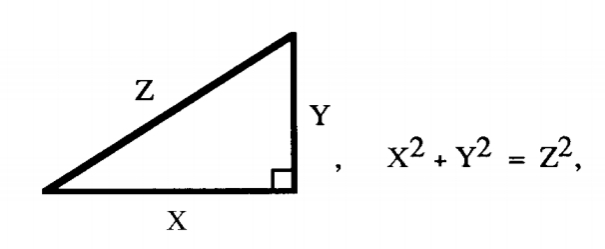
\includegraphics[width=10cm]{9.jpg}\\
			 % \caption{初}
		\end{figure}
	
		显然有$  (3,4,5)  $与$ (5,12,13) $等解.如何找全部整数解?等式$X^{2}+Y^{2}=Z^{2}$是齐次的,所以$ x=X/Z,y=Y/Z $就给出了圆$ C:(X^{2}+Y^{2}=1) \supset R^{2}$,它可以被参数化表示为:
		
		\begin{equation*}
			x=2 \lambda /\left(\lambda^{2}+1\right), y=\left(\lambda^{2}-1\right) /\left(\lambda^{2}+1\right),其中\lambda=x /(1-y)
		\end{equation*}
		
		
		所以下式可以给出所有解:
		
		
		\begin{equation*}
			X=2 \ell m, Y=\ell^{2}-m^{2}, Z=\ell^{2}+m^{2}\text { 其中 }\ell, m \in \mathbb{Z} \text { 互素 }
		\end{equation*}
	
	
		(若$ \ell,m $都是奇数,得到的$ X,Y,Z $值也可以各除以2).由于该等式为齐次,所以如果$ (X,Y,Z) $是一组解,那么$ (\lambda X,\lambda Y,\lambda Z) $也是一组解.
		
		
		在之前的几何教学中,我们已经对参数化有了相当的了解,并且通常我们都能很简单地判断参数化是否有效.而如果我们不是很了解参数化,我们可以通过下面的\textit{从定点出发的线性映射}来初步地理解:
	
	

		\begin{figure}[H]
		  \centering
		  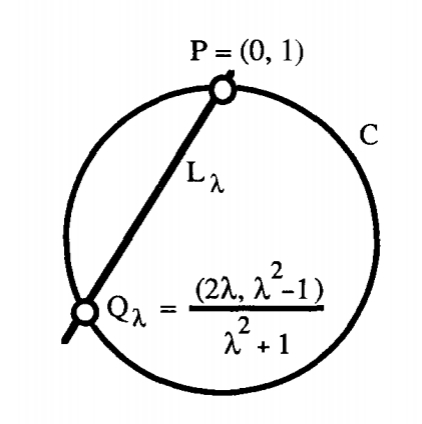
\includegraphics[width=6cm]{10.jpg}\\
		 % \caption{初}
		\end{figure}\par


		$ P=(0,1)\in C $,如果$\lambda \in Q$取任意值,那么穿过$ P $点斜率为$-\lambda$的直线$L_{\lambda}$与$ C $相交于另一点$Q_{\lambda}$.这种线性映射的映射结构会在以后的讨论中经常出现.
	
	\section{相似的例子}
		对于$ C:(2 X^{2} + Y^{2} =5 Z^{2}) $我们可以构造一个$ \mathbb{Z} \to C $的参数化的映射:
		
		\begin{equation*}
		x=\frac{2 \sqrt{5} \lambda}{1+2 \lambda^{2}}, \quad y=\frac{2 \lambda^{2}-1}{1+2 \lambda^{2}}
		\end{equation*}
		
		
		
		这样有助于我们理解C上所有实系数的点,而且和之前的例子没有本质上的区别.那么,如果是有理系数呢?
	
	
		\textbf{命题}\ 如果$ (a,b,c) \in \mathbb{Q} $满足$ 2a^{2}+b^{2}=5c^{2} $那么$ (a,b,c)=(0,0,0) $.
	
	
		\textbf{证明}\ 通过同时乘公分母与除以公因子,可以使得$ a,b,c $为整数,且他们不能同时为5的倍数.而如果$5\lvert a$且$ 5\lvert b $那么$ 25 \lvert c $,即$ 5 \lvert c $,这与上述题设矛盾.考虑$ a $和$ b $除以5的余数很容易得到矛盾:任何数的平方除以5后的余数只可能为0,1或4,即$2 a^{2}+b^{2}$除以5的余数只能是0+1,0+4,2+0,2+1,2+4,8+0,8+1以及8+4中的一个,而这些都不能写成$5 c^{2}$的形式.
	
	
		注意,这是一个完整的算数证明.
	\section{$\mathbb{Q}^{2}$中的圆锥曲线}
		$\mathbb{Q}^{2}$中的圆锥曲线是由二次方程$q(x,y)=ax^{2}+bxy+cy^{2}+dx+ey+f=0$给出的平面曲线.
	
	
		非退化的曲线有以下三种分类:
	
	
		1.椭圆$\dfrac{x^{2}}{a^{2}}+\dfrac{y^{2}}{b^{2}}=1$\indent
		2.抛物线$y=mx^{2}$\indent
		3.双曲线$\dfrac{x^{2}}{a^{2}}-\dfrac{y^{2}}{b^{2}}=1$
	
	
		此外,还有一些特殊情况:
	
	
		4.由$x^{2}+y^{2}=0$给出的单点.
	
	
		5.6.7.为三种类型方程给出的空集:5.$x^{2}+y^{2}=-1$ \indent  6.$x^{2}=-1$ \indent 7.$ 0=1 $.
		
		
		虽然这三种类型的方程都表示$R^{2}$上的空集,但是它们是不同的——例如考虑它们的复数解.
		
		
		8.一条直线:$ x=0 $.
		
		
		9.一对相交直线:$ xy=0 $.
		
		
		10.一对平行直线:$ x(x-1)=0 $.
		
		
		11.重合的直线:$x^{2}=0$.
		
		
		12.整个平面:$ 0=0 $.
	
	
	\section{射影平面$\mathbb{P}^{2}_{\mathbb{R}}$}
		\textbf{定义}
		\begin{equation*}
		\begin{aligned} \mathbb{P}^{2}_{\mathbb{R}}&= \mathbb{R}^{3} \text {中过原点的直线} \\ &=\{\text {比例} X : Y : Z\} \\ &=\left(\mathbb{R}^{3} \backslash\{0\}\right)/ \sim, \text { 其中 }(X, Y, Z) \sim(\lambda X, \lambda Y, \lambda Z), \lambda \in \mathbb{R} \backslash\{0\} \end{aligned}
		\end{equation*}
	
		(这里可以将$\mathbb{R}^{3}$推广到任意维的向量空间上)
	
	
	 	为了表示$ Z\neq0 $时的比例$ X:Y:Z $,可以设$x=\dfrac{X}{Z},y=\dfrac{Y}{Z}$,这样比例就相当于两个实数.换句话说,等价类$ (X:Y:Z) $有一个特殊的代表元$ (x:y:1) $.可是,在$ Z=0 $时,选择这种代表元的方式就无法实现了.这个讨论意味着$\mathbb{P}^{2}_{\mathbb{R}}$包含着一个$\mathbb{R}^{2}$,如图:
		\begin{figure}[H]
		  \centering
		  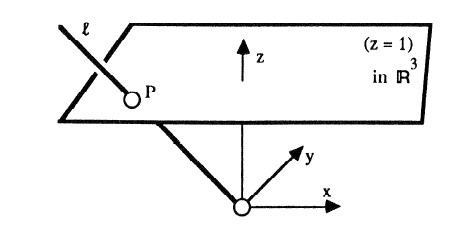
\includegraphics[width=10cm]{12.jpg}
		 % \caption{初}
		\end{figure}
	
		\vspace{-9mm}
		\begin{equation*}
		\mathbb{R}^{2} \hookrightarrow \mathbb{R}^{3} \backslash\{0\} \rightarrow \mathbb{P}^{2}_{\mathbb{R}} \text{由}(x, y) \mapsto(x, y, 1) \text{定义}
		\end{equation*}
		\vspace{5mm}
	
		$\mathbb{R}^{3}$中通过$ 0 $且不包含在平面($ Z=0 $)的直线都与平面($ Z=1 $)交于一点,这一点可以看做是等价类的代表元.而包含在平面($ Z=0 $) 中的直线与平面($ Z=1 $)无交点,所以他们不对应于$\mathbb{R}^{2}$中的点但对应于一个渐进方向,或者说对应于,$\mathbb{R}^{2}$中的一组平行线.所以可以认为$\mathbb{P}^{2}_{	\mathbb{R}}$是由$\mathbb{R}^{2}$和每组平行线方向上的无穷远点组成的.从这个角度来看,可以在$\mathbb{R}^{2}$中进行计算,通过某种渐进理论去猜想在无穷远点的情况,然后(如果必要的话),用齐次坐标去证明猜想.从$\mathbb{R}^{3}$中的直线来定义使之变得合理,因为这个定义平等地对待$\mathbb{P}^{2}_{\mathbb{R}}$上的所有点.
		
		
		变换群在整个几何中都是非常重要的,几何图形的性质要在一些变化类下保持不变才有意义.$\mathbb{R}^{2}$坐标中的仿射变换形式为$ T(x)=Ax+B $, 其中$x=(x,y)\in \mathbb{R}^{2}$,并且$ A $是一个$2\times2$的可逆矩阵,$ B $是一个平移向量;如果矩阵$ A $是正交矩阵,那么变换$ T $为欧式变换.每个非退化的曲线都可以通过欧式变换化成以上(1-3)的形式.
		
		
		$\mathbb{R}^{2}_{\mathbb{R}}$中的射影变化形式为$ T(x)=MX $,其中$ M $是一个$3\times3$的可逆矩阵.很容易理解这个变换在仿射片$\mathbb{R}^{2} \subset \mathbb{P}^{2}_{\mathbb{R}}$ 上的影响:作为一代部分定义的映射$\mathbb{R}^{2}\rightarrow \mathbb{R}^{2}$,这是一个分式线性变换
		
		\begin{equation*}
		\begin{pmatrix} x \\ y  \end{pmatrix}
		\mapsto (A\begin{pmatrix} x \\ y\end{pmatrix}+B)/(cx+dy+e)
		\end{equation*}
	
		其中,
		\begin{equation*}
		M=\begin{pmatrix} A  & B \\ c  d &e\end{pmatrix}
		\end{equation*}
	
		当$ cx+dy+e=0 $时,这个变换无定义.
	\section{平面曲线的方程}
		非齐次二次多项式
		
		\begin{equation*}
				q(x,y)=ax^{2}+bxy+cy^{2}+dx+ey+f
		\end{equation*}
	
		对应齐次二次方程式
		
		\begin{equation*}
			Q(X,Y,Z)=aX^{2}+bXY+cY^{2}+dXZ+eYZ+fZ^{2}
		\end{equation*}
		
		这种对应关系很容易理解为菜谱,或者你可以把它看作是由以下方面给出的双射$Q  \longleftrightarrow q$,
		\begin{equation*}
			q(x,y)=Q(X/Z,Y/Z,1) \text{其中} x=X/Z,y=Y/Z
		\end{equation*}
	
	
		反过来
		\begin{equation*}
			Q=Z^{2}q(X/Z,Y/Z)
		\end{equation*}
	
		平面曲线$C\subset \mathbb{P}^{2}$是由$ C:(Q(X,Y,Z)=0) $给出的曲线,其中$ Q $是齐次二次表达式;条件$ Q(X,Y,Z)=0 $在等价类上是良定义的,因为对任意的$\lambda \in \mathbb{R}, Q(\lambda X)=\lambda^{2}Q(X)$.
		
		
		\textbf{‘无穷远直线’与渐近方向}\ 
		$\mathbb{P}^{2}$中$ Z=0 $表示的点对应比例$ (X:Y:0) $,这些点形成了‘无穷远直线’$\mathbb{P}^{1}_{\mathbb{R}}=\mathbb{R} \cup \{ \infty \}$(因为$(X:Y)\mapsto X/Y$定义了一个双射$\mathbb{P}^{1}_{\mathbb{R}} \rightarrow \mathbb{R} \cup \{ \infty \}$)
		
		
		 $\mathbb{P}^{2}$中的直线是由$ L:(aX+bY+cZ=0) $定义的,并且通过$(X,Y,0)$ 的直线 $L\Longleftrightarrow aX+bY=0$. 在仿射坐标中,相同的直线是由$ ax+by+c=0 $给出的,从而使所有$a : b$比率相同的直线在无穷远处通过同一点. 这就是所谓的“平行线在无穷远处相遇”.
		
		
		\textbf{例子}:
		
		
		(a)\ $\mathbb{R}^{2}$中的双曲线($\frac{x^{2}}{a^{2}}-\frac{y^{2}}{b^{2}}=1$)对应于$\mathbb{P}^{2}_{\mathbb{R}}$中的C:($\frac{X^{2}}{a^{2}}-\frac{Y^{2}}{b^{2}}=Z^{2}$);很明显,在$(b,±a,0)\in \mathbb{P}^{2}_{\mathbb{R}}$的两点满足$ (Z=0) $,这两个点对应于双曲线的渐近线.
		
		
		注意,在$\mathbb{P}^{2}_{\mathbb{R}}$的仿射片($X\neq 0$)中, 仿射坐标是$ u=Y/X,v=Z/X $,这样C就变成了椭圆($\frac{u^{2}}{b^{2}}+v^{2}=\frac{1}{a^{2}}$).
		
		
		(b)\ $\mathbb{R}^{2}$中的抛物线($y=mx^{2}$)对应于$\mathbb{P}^{2}_{\mathbb{R}}$中的$C:(YZ=mX^{2}$);在单点$ (0,1,0) $处满足$ Z=0 $. 因此在$\mathbb{P}^{2}$中,“抛物线的两个分支在无穷远处相遇”.
	
	
	\section{$\mathbb{P}^{2}$中平面曲线的分类}
		k是一个特征不为2的域,回想二次型线性代数的两个结果:
		
		
		\textbf{命题(A)}\ 有天然的双射$\{ \text{二次齐次多项式} \}=\{\text{二次型}k^{3} \to k \} \longleftrightarrow \{k^{3}\text{上的对称双线性型}\}$,并且可以由下式给出:
		\begin{equation*}
		aX^{2}+2bXY+cY^{2}+2dXZ+2eYZ+fZ^{2} \longleftrightarrow \begin{bmatrix} a & b &d \\ b & c &e\\ d & e & f\end{bmatrix}
		\end{equation*}
		如果相应的双线性型是非退化的,则二次型是非退化的,就是说,这个矩阵是非奇异的.
		
		
		\textbf{定理(B)}\ $ V $是$ k $上的向量空间,$Q:V\to k\text{是二次型},\text{则存在一组}V\text{的基使}Q=\varepsilon_{1}x^{2}_{1}+\varepsilon_{2}x^{2}_{2}+\cdots\varepsilon_{n}x^{2}_{n}$,其中$\varepsilon_{i}\in k$.(格拉姆-施密特正交化证明了这一点)
		
		
		\textbf{推论}\ 在适当的坐标系中,$\mathbb{P}^{2}_{\mathbb{R}}$中的任何圆锥曲线都是下列情况之一:
		
			
		(1)非退化曲线, $C:(X^{2}+Y^{2}-Z^{2}=0)$;
		
		
		(2)空集, $(X^{2}+Y^{2}+Z^{2}=0)$;
		
		
		(3)交叉线对, $(X^{2}-Y^{2}=0)$;
		
		
		(4)一个点$(0,0,1)$, $(X^{2}+Y^{2}=0)$;
		
		
		(5)重叠线$(X^{2}=0)$;
		
		
		(可以将$\mathbb{P}^{2}_{\mathbb{R}}$整个平面由$ (0=0) $给出.)
		
	
		\textbf{证明}\ 任何实数$\varepsilon$ 是0或$\pm \sqrt{a}$, 因此我们只需要考虑定理中$\varepsilon=0$或$\pm1$的Q. 另外, 由于我们只对轨迹$ (Q = 0) $感兴趣, 所以我们可以把Q乘以-1,这将立即得出给定的列表.
		
		
		关于这个推论有两点: 首先, 列表比$ (1.3) $中的要短得多: 例如, $ (1.3) $的3个非退化情况(椭圆、抛物线、双曲线)都对应情况(1). 在射影情形下不区分交叉和平行的线对这两种情况. 其次, 从一般代数学原理推导出以上几种情况更简单一点.
	\section{曲线参数化}
		设$ C $是$\mathbb{P}^{2}_{\mathbb{R}}$中的非退化的非空二次曲线. 由推论$ 1.6 $, 取新的坐标$ (X+Z, Y, Z-X) $, $ C $与曲线$(XZ=Y^{2})$在投影上等价, 这个曲线的参数化是
	
		\begin{equation*}
		\begin{array}{l}{\Phi : \mathbb{P}^1_{\mathbb{R}}\quad \longrightarrow \quad C \subset \mathbb{P}^{2}_{\mathbb{R}}} \\ {(U : V) \quad\longmapsto\quad  \left(U^{2} : UV : V^{2}\right)}\end{array}
		\end{equation*}

		\textbf{备注}
		
		
	 	1. 逆映射$\Psi: C\longrightarrow \mathbb{P}^{1}_{\mathbb{R}}$由$(X:Y:Z)\longmapsto(X:Y)=(Y:Z)$给出;如果 $Y \neq 0$,就按左边的比例定义, 如果 $Z \neq 0$, 就按右边的比例定义.在后面要介绍的术语中,$\Phi$ 和$\Psi$ 是变换的逆同构.
	
	
		2.任意非空的非退化二次曲线默认为投影等价于$(XZ-Y^{2})$;在特征不为2的域中,这在练习5中是合理的(对特征为2的域感兴趣的读者应该把这个作为非退化二次曲线的定义).
	\section{2个变量的齐次型}
		设$ F(U, V) $为关于$ U, V $的$ d $次非零齐次多项式, 系数在固定的域$ k $内
		
		\begin{equation*}
		F(U,V)=a_{d}U^{d}+a_{d-1}U^{d-1}V+...+a_{i}U^{i}V^{d-i}+...a_{0}V^{d}
		\end{equation*}
		
		F有一个与之相关的单变量非齐次多项式:
		
		\begin{equation*}
			f(u)=a_{d}u^{d}+a_{d-1}u^{d-1}+...+a_{i}u^{i}+...a_{0}
		\end{equation*}
		
		显然对于$ \alpha \in k $,有
		\begin{equation*}
		f(\alpha )=0 \Leftrightarrow (u-\alpha)|f(u)\Leftrightarrow (U-\alpha V)|F(U,V)\Leftrightarrow F(\alpha,1)=0
		\end{equation*}
		
		所以$ f $的零点对应于$ F $在$\mathbb{P}^{1}$上除点$ (1,0) $的零点,而点$ (1,0) $对应于‘点$\alpha =\infty$’.$ F $在无穷远处有一个零点是什么意思?
		
		\begin{equation*}
			F(1,0)=0\Leftrightarrow a_{d}=0\Leftrightarrow deg f<d
		\end{equation*}
		
		现在定义$ F $在$\mathbb{P}^{1}$上零点的重数为
		
		
		(i) $\alpha \in k$在f中的重数;
		
		
		(ii)如果$ (1,0) $是零点,重数为$ d-deg f $.
		
		
		所以$ F $在$ (\alpha,1) $处的零点重数是$ (U-\alpha V) $除$ F $的最大幂, 在$ (1,0) $处是$ V $除$ F $的最大幂.
		
	
		\textbf{命题}\ 设$ F(U,V) $是$ U,V $的$ d $次的非零齐次多项式, 那么$ F $在$\mathbb{P}^{1}$上最多有$ d $个零点;此外,如果$ k $是代数闭域, 那么$ F $在$\mathbb{P}^{1}$上恰好有$ d $个零点, 前提是这些数要用上面定义的乘法来计算.
		
		
		\textbf{证明}\ 令$m_{\infty}$为$ F $在$ (1,0) $处的零点重数;然后根据定义, $d-m_{\infty}$是非齐次多项式$ f $的次数, 然后这个命题可以归结为一个众所周知的事实,即单变量多项式最多有$ deg f $个根.
		
		
		注意,在代数封闭域上, $ F $将分解为线性型$\lambda_{i}=(a_{i}U+b_{i}V)$的乘积$F=\Pi\lambda_{i}^{m_{i}}$,用这种方法处理,点$ (1,0) $ 对应于形式$\lambda_{\infty}=V$,并且与所有其他点处于相同的地位.
	\section{贝祖定理的简单情况}
		贝祖定理指出, 如果$ C $和$ D $是次数为$ deg C=m, deg D=n $的平面曲线,并且$ (i) $域是代数闭的;$ (ii) $交点个数按重数来计数;$ (iii)  $我们在$\mathbb{P}^{2}$中计算, 所以考虑无穷远处的交点. 则$ C $和$ D $的交点个数为$ mn $. 在本节中, 将在其中一条曲线是直线或二次曲线的情况下证明.
		
		
		\textbf{定理}\ 设$L\subset \mathbb{P}^{2}_{k}$是一条直线(相应的,$C\subset \mathbb{P}^{2}_{k}$是一条非退化二次曲线), $D\subset \mathbb{P}^{2}_{k}$是由$D:(G_{d}(X,Y,Z)=0)$ 定义的一条曲线, 其中$ G $是关于$ X, Y, Z $的$ d $次齐次多项式. 假定 $ L $不包含于 $ D $(相应的,$ C $ 不包含于$ D $); 则$ L $与$ D $的交点个数$\# \{L\cap D\}\leq d $ (相应的,$\# \{C\cap D\}\leq 2d $).
		
		
		事实上, 对于交点的重数有一个自然的定义, 使得对于用重性计数的交点的个数, 不等式仍然成立, 如果$ k $是代数闭的, 那么等式成立.
		
		
		\textbf{证明}\ $\lambda$ 为线性型, 由 $\lambda=0$ 给出的一条直线$L\subset \mathbb{P}^{2}_{k}$, 将其按下面方式参数化
		
		\begin{equation*}
			X=a(U,V), Y=b(U,V), Z=c(U,V)
		\end{equation*}
	
		其中$ a,b,c $是$ U,V $的线性型.例如, 如果$\lambda=\alpha X+\beta Y+\gamma Z$, 且$\gamma \neq 0$, 那么$ L $可以参数化为$ X=U,Y=V, Z=-\dfrac{\alpha}{\gamma}U-\dfrac{\beta}{\gamma}V$. 类似的, 正如$ (1.7) $中证明的, 非退化曲线可以参数化为$ X=a(U,V), Y==b(U,V),Z=c(U,V) $.其中$ a,b,c $是$ U,V $中的二次型,这是因为$ C $是$(XZ=Y^{2})$的射影变换, 它的参数化方式为$ (X,Y,Z)=(U^{2},UV,v^{2})$,所以$ C $是
		
		\begin{equation*}
		 \begin{bmatrix} X \\Y\\ Z\end{bmatrix}=M\begin{bmatrix} U^{2} \\UV\\ V^{2}\end{bmatrix}
		\end{equation*}
	
		其中$ M $是$ 3\times3 $非奇异矩阵.
	
		\begin{figure}[H]
		  \centering
		  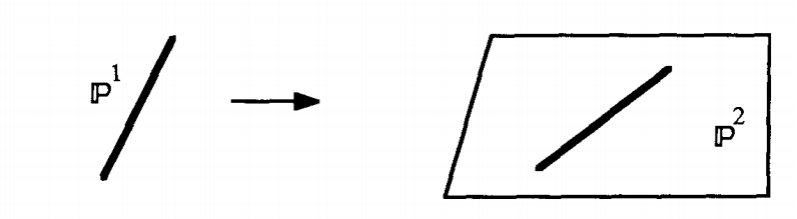
\includegraphics[width=7cm]{1811.jpg}参数化直线\\
		  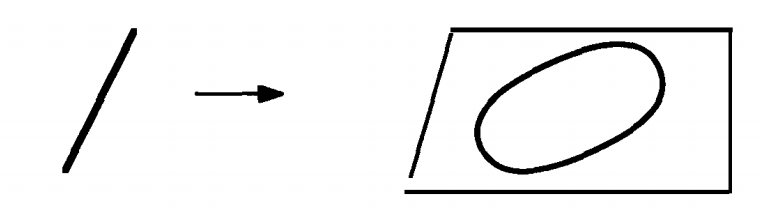
\includegraphics[width=7cm]{1822.jpg}参数化二次曲线\\
		 % \caption{初}
		\end{figure}
	
		然后通过$F(U:V)=G_{d}(a(U,V),b(U,V),c(U,V))=0$求出$ (U:V) $的比值, 求出$ L $(相应的,曲线$ C $)与$ D $的交点.但$ F $是关于$ U,V $的$ d $(相应的,$ 2d $)次的齐次多项式, 因此可参考$ (1.8) $得出结果.

	\section{推论}
		如果$P_{1},...,P_{5} \in \mathbb{P}^{2}_{\mathbb{R}}$是任意四点不共线的5个点,那么就至多存在一条圆锥曲线穿过$P_{1},...,P_{5}$.
		
		
		\textbf{证明} 用反证法假设$C_{1}$和$C_{2}$是两条不相同的圆锥曲线使得
		\begin{equation*}
		C_{1} \cap C_{2} \supset \{ P_{1},...,P_{5}\}
		\end{equation*}
	
		$C_{1}$是非空的因此它是非退化的,那么,由$ (1.7) $,它投影地等价于参数化的圆锥曲线
		
		\begin{equation*}
		C_{1}=\{(U^{2},UV,V^{2}) \mid (U,V)\in P^{1}\}
		\end{equation*}
	
		由(1.9),$C_{1} \subset C_{2}$.那么,如果$Q_{2}$与$C_{2}$相等,那么$Q_{2}(U^{2},UV,V^{2})\equiv 0$对于任何$(U,V)\in \mathbb{P}^{1}$成立,并且通过简单计算(见\textit{习题 1.6 })就可以看出$Q_{2}$是$(XZ-Y^{2})$的倍数,这与$C_{1}\ne C_{2}$相矛盾.
		
		
		现在假设$C_{1}$是退化的,由(1.6)可知,它是一组线对或是一条线,而且很明显有
		
		\begin{equation*}
		C_{1}=L_{0}\cup L_{1},C_{2}=L_{0}\cup L_{2}
		\end{equation*}
	
		其中$ L_{1} L_{2} $是不同的线.那么$C_{1}\cap C_{2}=L_{0}\cup (L_{1}\cap L_{2})$
	\begin{figure}[H]
	  \centering
	  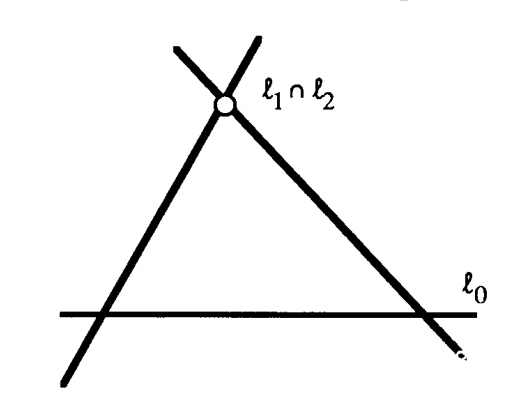
\includegraphics[width=6cm]{19.jpg}
	 % \caption{初}
	\end{figure}
		因此,$P_{1}...P_{5}$中的4点在$P_{0}$上,矛盾.则证毕.
		
	\section{所有二次曲线的空间}
		$S_{2}=\{\mathbb{R}^{3} \text{中的二次型}\}=\{3\times3\text{对称矩阵}\}\cong \mathbb{R}^{6}$, 如果$Q\in S_{2}$,记 $Q=aX^{2}+2bXY+\cdots fZ^{2}$;则对于$P_{0}=(X_{0},Y_{0},Z_{0})\in \mathbb{P}^{2}_{\mathbb{R}}$, 考虑到$P_{0}\in C:(Q=0)$的关系,这具有形式$Q(X_{0},Y_{0},Z_{0})=aX^{2}_{0}+2bX_{0}Y_{0}+\cdots fZ_{0}^{2}=0$, 对于固定的$P_{0}$, 这是关于$(a,b,\cdots f)$ 的线性方程. 所以$S_{2}(P_{0})=\{Q\in S_{2}|Q(P_{0})=0\}\cong \mathbb{R}^{5}\subset S_{2}=\mathbb{R}^{6}$是一个5维的超平面.
		
		
		对于$P_{1},\cdots P_{n}\in \mathbb{P}^{2}_{\mathbb{R}}$, 类似地定义$S_{2}(P_{1},\cdots P_{n})=\{Q\in S_{2}|Q(P_{i})=0 \text{其中} i=1,\cdots n\}$;所以可以得到关于$ Q $的6个系数$(a,b,\cdots f)$的$ n $个线性方程. 这得出了以下结果:
		
		
		\textbf{命题}\ $dimS_{2}(P_{1},\cdots P_{n})\geq6-n$.
		
		
		如果$P_{1},\cdots P_{n}$能都满足以些条件,我们也可以期望等式成立, 更准确地说应该是:
		
		
		\textbf{推论}\ 如果$n\leq5$并且$P_{1},\cdots P_{n}$中任意4点不共线,则$dimS_{2}(P_{1},\cdots P_{n})=6-n$.
		
		
		\textbf{证明}\ 推论1.10表明, 如果n = 5, $dim S_{2}(P_{1},\cdots P_{n})\leq1$,给出了这种情况的证明.如果$n\leq4$, 然后我可以加入点$P_{n+1},\cdots,P_{5}$ 并且保持没有4个点共线的条件, 由于每个点最多增加一个线性条件, 所以$1=dimS_{2}(P_{1},\cdots P_{5})\geq dimS_{2}(P_{1},\cdots P_{n})-(5-n)$.
		
		
		请注意, 如果给定6个点$P_{1},\cdots P_{6} \in \mathbb{P}^{2}_{\mathbb{R}}$, 可能存在在一条圆锥曲线同时包含这6个点, 也可能不存在.
		
	\section{两条圆锥曲线的交点}
		\begin{figure}[H]
		  \centering
		  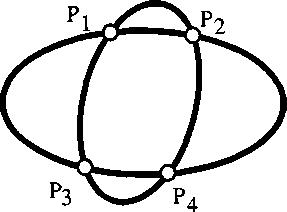
\includegraphics[width=5cm]{20.jpg}\\
		 % \caption{初}
		\end{figure}
		正如我们上面所看到的, 两个二次曲线经常会在4个点相交;相反, 根据推论$ (1.11) $, 给定4个点$P_{1},\cdots P_{4}\in \mathbb{P}^{2}$, 在适当条件下$S_{2}(P_{1},\cdots P_{4})$是一个二维向量空间,因此选择$S_{2}(P_{1},\cdots P_{4})$的一组基$Q_{1},Q_{2}$给出了2条二次曲线$C_{1},C_{2},$ 使得$C_{1}\cap C_{2}=\{P^{1},\cdots P^{4}\}$.
		
		
		这里还有许多非退化曲线多重交点的可能性:
		\begin{figure}[H]
		  \centering
		  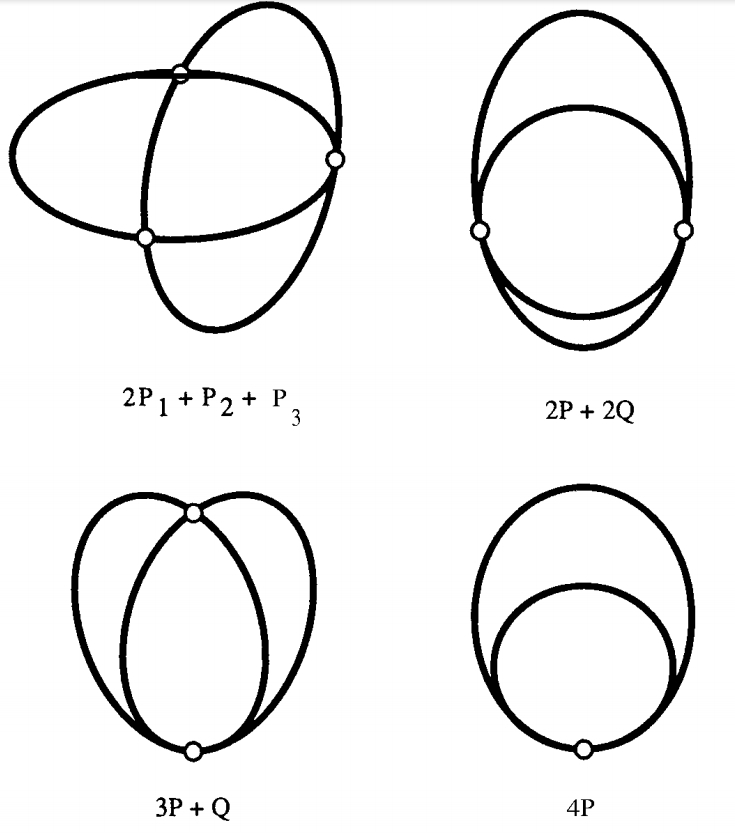
\includegraphics[width=8cm]{21.jpg}
		 % \caption{初}
		\end{figure}
	
	
		\textit{有关合适的方程式见练习1.9a}
		
		\section{退化的圆锥曲线族}
		\textbf{定义}\ \textit{圆锥曲线族}是一类满足以下特点的齐次多项式:
		
		\begin{equation*}
		C_{(\lambda, \mu)} :\left(\lambda Q_{1}+\mu Q_{2}=0\right)
		\end{equation*}
		
		其中的每一个元素都是一条由参数$(\lambda, \mu)$线性控制的平面圆锥曲线.类似于我们在$\mathbb{P}^{1}$上做的那样,我们可以用一个比例$(\lambda : \mu)$来代表对应的平面圆锥曲线.
		
		
		如示例中,只有当$(\lambda : \mu)$为一个特殊值时,平面圆锥曲线$C_{(\lambda, \mu)}$才是退化的.事实上,如果将二次齐次多项式$Q$对应的$3 \times 3$对称矩阵的行列式记作$\operatorname{det}(Q)$,那么显然有
		\begin{equation*}
		C_{(\lambda, \mu)} \text {是退化的} \Longleftrightarrow \operatorname{det}\left(\lambda Q_{1}+\mu Q_{2}\right)=0
		\end{equation*}
		
		
		将对称矩阵$Q_{1}$和$Q_{2}$表述的条件记作:
		\begin{equation*}
		F(\lambda, \mu)=\operatorname{det}\left|\lambda\left[\begin{array}{ccc}{a} & {b} & {d} \\ {b} & {c} & {e} \\ {d} & {e} & {f}\end{array}\right]+\mu\left[\begin{array}{ccc}{a^{\prime}} & {b^{\prime}} & {d^{\prime}} \\ {b^{\prime}} & {c^{\prime}} & {e^{\prime}} \\ {d^{\prime}} & {e^{\prime}} & {f^{\prime}}\end{array}\right]\right|=0
		\end{equation*}
		
		
		那么就可以注意到$F(\lambda, \mu)$是一个对于$\lambda, \mu$的三次齐次多项式,那么我们就可以对$F$应用$(1.8)$的结论:
		
	
		\textbf{命题} \ 假设$C_{(\lambda, \mu)}$是在$\mathbb{P}^{2}_{k}$上的一族圆锥曲线,并且这一族圆锥曲线至少有一个非退化的(因此$F(\lambda, \mu)$不总是0),那么这一族中最多有三个退化的圆锥曲线.另外,如果有$k=\mathbb{R}$,那么这一族最少有一个退化的圆锥曲线.
		
		
		\textbf{证明} \ 一个三次齐次多项式的零点个数$\leq 3$.而在$\mathbb{R}$上,它最少有一个零点.

	\section{一些实例}
		令$P_{1} \ldots P_{4}$是$\mathbb{P}^{2}_{\mathbb{R}}$上任意三个不共线的四点,则经过这四点的圆锥曲线族$C_{(\lambda, \mu)}$有三个退化的元素,即线对$L_{12}+L_{34}, L_{13}+L_{24}, L_{14}+L_{23}$,其中$L_{ij}$是过$P_{i},P_{j}$的直线:
		\begin{figure}[H]
		  \centering
		  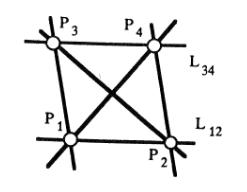
\includegraphics[width=5cm]{22.jpg}
		 % \caption{初}
		\end{figure}
	
	
		{然后,我们假设这一族圆锥曲线是由$Q_{1}=Y^{2}+r Y+s X+t$和$Q_{2}=Y-X^{2}$生成的,并寻找$P_{1} \ldots P_{4}$这四个交点.}
		
		\begin{figure}[H]
		  \centering
		  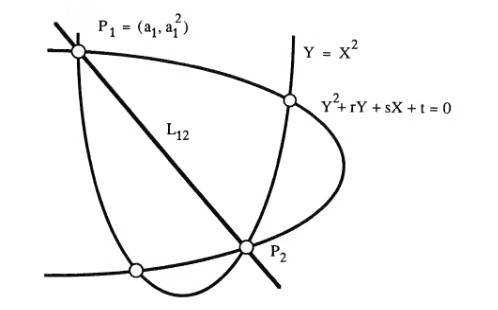
\includegraphics[width=8cm]{23.jpg}
		 % \caption{初}
		\end{figure}
	
	
		通过下列步骤可解:
		
		
		$(1)$找出三个比例$(\lambda : \mu)$使得$C_{(\lambda, \mu)}$是退化的圆锥曲线.根据上文,这意味着我们需要找到三次齐次多项式的三个根
		\begin{equation*}
			\begin{aligned} F(\lambda, \mu) &=\operatorname{det}\left|\lambda\left[\begin{array}{ccc}{0} & {0} & {s / 2} \\ {0} & {1} & {r / 2} \\ {s / 2} & {r / 2} & {t}\end{array}\right]+\mu\left[\begin{array}{ccc}{-1} & {0} & {0} \\ {0} & {0} & {1 / 2} \\ {0} & {1 / 2} & {0}\end{array}\right]\right| \\ &=-\frac{1}{4}\left(s^{2} \lambda^{3}+\left(4 t-r^{2}\right) \lambda^{2} \mu-2 r \lambda \mu^{2}-\mu^{3}\right) \end{aligned}
		\end{equation*}
		
		
		$(2)$从退化的圆锥曲线中分出2条作为线对(这意味着解两个四次方程).
		
		
		$(3)$这四个交点$P_{i}$就是线的交点.
		
		
		这个步骤给出了利用伽罗瓦理论解四次方程的一个几何解释:设$k$是一个域,而$f(X)=X^{4}+r X^{2}+s X+t \in k[X]$是一个四次多项式.则两条抛物线$C_{1}$和$C_{2}$相交于四个点$P_{i}=\left(a_{i}, a_{i}^{2}\right)(i = 1\ldots4)$,而$a_{i}$是$f$的四个根.
		
		
		则直线$L_{ij}=P_{i} P_{j}$由下式给出:
		\begin{equation*}
			L_{ij} :\left(Y=\left(a_{i}+a_{j}\right) X-a_{i} a_{j}\right)
		\end{equation*}
		
		而可约的圆锥曲线$L_{12}+L_{34}$由下式给出:
		\begin{equation*}
			Y^{2}+\left(a_{1} a_{2}+a_{3} a_{4}\right) Y+\left(a_{1}+a_{2}\right)\left(a_{3}+a_{4}\right) X^{2}+s X+t=0
		\end{equation*}
	
		这是由$Q_{1}-\left(a_{1}+a_{2}\right)\left(a_{3}+a_{4}\right) Q_{2}=0$推出的.因此,使圆锥曲线$\lambda Q_{1}+\mu Q_{2}$退化为线对的3个比例$(\lambda : \mu)$的值为:
		
		\begin{equation*}
			-\left(a_{1}+a_{2}\right)\left(a_{3}+a_{4}\right),-\left(a_{1}+a_{3}\right)\left(a_{2}+a_{4}\right),-\left(a_{1}+a_{4}\right)\left(a_{2}+a_{3}\right)
		\end{equation*}
		根是这三个数的三次方程被称为与四次方程对应的\textit{辅三次方程};这可以通过初等对称函数的理论计算得到;因此这是一个极具可操作性的步骤.而在另一方面,上面给出的概要优雅地给出了仅有三阶行列式的辅三次方程的一个推导.
		
	\section*{练习1}
		\subsection{考虑通过$ (-1,-2) $的直线,将二次曲线$C:(x^{2}+y^{2}=5)$参数化.并找出$(x^{2}+y^{2}=5)$的所有有理解.}
			解:由
				\begin{equation*}
				  \left\{
				   \begin{aligned}
				 x^{2}+y^{2} &=5 \\
				 y+2= &k(x+1)\\
				   \end{aligned}
				   \right.
				\end{equation*}
			得
				\begin{equation*}
				  \left\{
				   \begin{aligned}
				  x &=\frac{-k^{2}+4k+1}{1+k^{2}} \\
				  y &=\frac{2k^{2}+2k-2}{1+k^{2}}\\
				   \end{aligned}
				   \right.
				\end{equation*}
			
			
			若(a,b)是$(x^{2}+y^{2}=5)$的解, 则$ (-a,-b),(-a,b),(a,-b) $也是$(x^{2}+y^{2}=5)$的解. 所以不妨找$a>0, b>0$的有理解, 由上述参数化知,$ (x,y) $是有理点$\Leftrightarrow k\in Q$, $x>0, y>0\Leftrightarrow \frac{2}{\sqrt{5}+1}<k<\sqrt{5}+2$
			
		\subsection{p是质数,猜想$x^{2}+y^{2}=p$有有理解的充要条件,证明你的猜想. }
			(若$x^{2}=a(mod \ p)$有解,称a是模p 的二次剩余.数论里的一个基本结论, -1是模$ p $ 的二次剩余当且仅当$ p=2 $或$ p=1mod16 $. )
			
			解:猜想$ p=2 $或$ p=1mod 4 $
			
			
			 $x^{2}+y^{2}=p$有有理解, $x=\frac{a}{c},y=\frac{b}{c},\Leftrightarrow a^{2}+b^{2}=pc^{2}$有整数解.
			
			$"\Rightarrow"$ \ a是模$ p $的二次剩余$\Leftrightarrow a^{\frac{p-1}{2}}=1(mod \ p)$, 显然1一定是模$ p $的二次剩余(因为$a^{\frac{p-1}{2}}=1(mod \ p)$),所以$x^{2}=1(mod \ p)$有解. 若$ (a,b,c) $满足$a^{2}+b^{2}=pc^{2}$, 则一定满足$a^{2}+b^{2}=pc^{2}(mod \ p)$. 因为一定存在$ a $, 使$a^{2}=1(mod \ p)$,所以一定存在$ b $使$b^{2}=-1(mod \ p)$, 得$ p=2 $或$ p=1mod4 $.
			
			$"\Leftarrow"$ \ $ p=2 $时, $1^{2}+1^{2}=2$, 所以$ (1,1) $是 $x^{2}+y^{2}=2$的有理解.
			
			$ p=1mod  4 $时,$ p=4k+1 , k \in Z$
			$a^{2}=1,0(mod 4),b^{2}=1,0(mod 4)$, 所以$a^{2}+b^{2}=pc^{2}=1,2(mod 4)$,
			即$a^{2}+b^{2}=pc^{2}=4k^{2}+1,4k^{2}+2$, 而$pc^{2}=(4k+1)c^{2}=4kc^{2}+c^{2}=c^{2}(mod 4)=1,2$,
		\subsection{证明1.3中的陈述:仿射变换可以将任何一条圆锥曲线变为1-12中的形式.}
		
		
			解答:使用线性变换$ x \mapsto Ax $把$ax^{2}+bxy+cy^{2}$的部分转换为$\pm x^{2} \pm y^{2},\pm x^{2}$或0的形式;然后再通过配方将尽可能多的线性部分消除
		\subsection{对1.3中的仿射圆锥曲线和1.6中的射影圆锥曲线进行详细的比较}
			解答:(1).非退化圆锥曲线,对应椭圆、抛物线、双曲线;
			
			
			(2).空集,对应1.3中4、5、6三种情况;
			
			
			(3).线对,对应7、8、9三种情况;
			
			
			(4).单点,对应4;
			
			
			(5).双线,对应10;
			
			
			另外,视情况,可认为整个射影平面对应0=0;
			
			
			将1.3的多项式所对应的矩阵化为只由1和-1组成的对角形式的矩阵,则1.6中从上到下的式子分别对应:
			$\begin{bmatrix}
			    1&0&0\\
			    0&1&0\\
			    0&0&-1\\
			\end{bmatrix}
			\begin{bmatrix}
			    1&0&0\\
			    0&1&0\\
			    0&0&1\\
			\end{bmatrix}
			\begin{bmatrix}
			    1&0&0\\
			    0&-1&0\\
			    0&0&0\\
			\end{bmatrix}
			\begin{bmatrix}
			    1&0&0\\
			    0&1&0\\
			    0&0&0\\
			\end{bmatrix}
			\begin{bmatrix}
			    1&0&0\\
			    0&0&0\\
			    0&0&0\\
			\end{bmatrix}$
		\subsection{$ k $为特征值不为2的任意数域,$ V $是$ k $上的三维向量空间,$ Q:V \to k $是一个V上的非退化的二次型.请证明如果$ 0 \ne e_{1} \in V $满足$ Q(e_{1} )=0 $那么V有基底$e_{1},e_{2},e_{3}$使得$ Q(x_{1} e_{1} + x_{2} e_{2} + x_{3} e_{3} )= x_{1} x_{3} +a x_{2}^{2}$.}
			解答:设一对称双线性型满足:
				$\varphi(\alpha,\beta)=\alpha 'A \beta$ (之后简写为($\alpha,\beta$))
				
				
				$ Q(e_{1} )=0 \Rightarrow \varphi (e_{1},e_{1} )=0 $
				
				
				$\varphi(e_{1},e_{3})=1$
				
				
				则$Q(x_{1} e_{1}+x_{2} e_{2}+x_{3} e_{3} )= \varphi (x_{1} e_{1}+x_{2} e_{2}+x_{3} e_{3},x_{1} e_{1}+x_{2} e_{2}+x_{3} e_{3} )
				=2 x_{1} x_{2}(e_{1},e_{3} )+2 x_{1} x_{3}+x_{2}^{2}(e_{2},e_{2} )+ x_{3}^{2}(e_{3},e_{3})+2 x_{2} x_{3}(e_{2},e_{3})$
				
				
				下证$\exists e_{2} \ne 0$使得$(e_{1},e_{2} )=0;(e_{2},e_{3} )=0;(e_{2},e_{2})\ne 0$
				
				
				首先
				\begin{equation*}
				\left\{\begin{aligned}\left(e_{1}, e_{2}\right) &=0 \\\left(e_{3}, e_{2}\right) &=0 \end{aligned} \Rightarrow\left\{\begin{array}{l}{\left(x_{1} y_{1} z_{1}\right) A e_{2}=0} \\ {\left(x_{3} y_{3} z_{3}\right) A e_{2}=0}\end{array}\right.\right. \text{有解}
				\end{equation*}
			%	下面两行在一个大括号里
			%	($e_{1}$,$e_{2}$)=0\\
			%	($e_{3}$,$e_{2}$)=0
			%	
			%	$\Rightarrow$
			%	
			%	下面两行在一个大括号里
			%	($x_{1}$$y_{1}$$z_{1}$)A$e_{2}$=0
			%	($x_{3}$$y_{3}$$z_{3}$)A$e_{2}$=0
			%	有解
				
				$\begin{bmatrix}
				    (x_{1}y_{1}z_{1})A\\
				    (x_{3}y_{3}z_{3})A\\
				\end{bmatrix}$
				秩$\le 2$,解空间维数$\ge 1$
				
				
				$(e_{1},e_{2})=0,(e_{3},e_{2})=0$
				
				
				若$(e_{2},e_{2})=0,e_{2}=0$得出矛盾
				
				
				故$e_{2}\ne 0$
				
				
				可得$Q(x_{1} e_{1} + x_{2} e_{2}+x_{3} e_{3} )=2 x_{1}x_{3}+x_{2}^{2} (e_{2},e_{2} )+ x_{3}^{2}(e_{3},e_{3} )$
				
				
				$e_{3}'=\lambda e_{1}+\mu e_{3}$(令$\mu=1$)$\Rightarrow e_{3} '=- \frac{e_{2}e_{3}}{2} e_{1}+e_{3}$
				
				
				最后再取$e_{1}'= \frac{1}{\sqrt{2}} e_{1},e_{3} ''= \frac{1}{\sqrt{2}} e_{3}'$
				
				
				得证
		\subsection{设k是一个至少有4个元素的域,$C:(XZ=Y^{2})\supset P^{2}_{k}$.证明:如果$ Q(X,Y,Z) $是在C上为0的二次型,则$ Q=\lambda(XZ-Y^{2}) $.}
			解答:带入特殊点即可,可得Q所对应的矩阵为
			$\begin{bmatrix}
			    0&0&\lambda\\
			    0&-2\lambda&0\\
			    \lambda&0&0\\
			\end{bmatrix}$
		\subsection{在$ \mathbb{R}^{3} $上,考虑$ A:(Z = 1) $和$ B:(X = 1) $两个平面,一条过原点的直线交平面$ A $于$ (x,y,1) $,交平面$ B $于 $ (1,\dfrac{y}{x},\dfrac{1}{x}) $.考虑由$(x, y) \mapsto\left(y^{\prime}=\dfrac{y}{x}, z^{\prime}=\dfrac{1}{x}\right)$定义的映射 ,当原象为\\
		(1)直线族$ ax = y + b $ (其中$ a $是定值而$ b $是变量)\\
		(2)圆$(x-1)^{2}+y^{2}=c$其中c是变量(注意$ c $的取值)\\
		时,考虑它的象.并且指出当映射或逆映射没有定义时的情况.}
		
			解答:
			(1)设参数$ t $,则有$ ax = y + b $交$ A:(Z = 1) $于$ (t,at-b,1) $,参考题干给出的映射,直线在$ B:(X = 1) $上为$ (1,\dfrac{at-b}{t},\dfrac{1}{t}) $.则映射下的象为$ bz' = -y' + a $.显然,映射和逆映射总有定义.
			
			
			(2)设参数$ \theta $,取$ x = 1 + c\cos\theta,y = c\sin\theta $,参考题干给出的映射,有$ y' = \dfrac{c\sin\theta}{1+c\cos\theta},z' = \dfrac{1}{1+c\cos\theta} $.则映射下的象为$ y'^{2} = (c^{2}-1)z'^{2} +2z' -1 $,当$ c<1 $时是椭圆,当$ c = 1 $时是抛物线,当$ c>1 $时是双曲线.当映射没有定义时,有$ x = 0 $,即圆与$ A:(Z = 1) $的交点为$ (0,y,1) $;当逆映射没有定义时,有$ x = \infty $,即圆与$ A:(Z = 1) $ 的交点为$ (\infty,y,1) $.
		
		\subsection{$ P_{1},\cdots P_{4} $是$ \mathbb{P}^{2} $上任意三点不共线的四点.证明:存在一个仿射坐标系使得这四个点的坐标分别为$ (1,0,0),(0,1,0),(0,0,1) $和$ (1,1,1) $,设$ P_{5} = (a,b,c)$是这四个点以外的第五个点,找到所有经过这五个点的圆锥曲线并给出推论1.10和引理1.11的另外一个证明.}
		
			解答:设$ P_{1},\cdots P_{4} $的坐标为$ (x_{i},y_{i},1) ,i = 1,\cdots 4$.考虑$ (x_{i},y_{i},1) ,i = 1,\cdots 4$到$ (1,0,0),(0,1,0),(0,0,1),(1,1,1) $的仿射变换$ Ax +b = y $,则有
			
			
			$\left(\begin{array}{lll}{a_{11}} & {a_{12}} & {a_{33}} \\ {a_{21}} & {a_{22}} & {a_{23}} \\ {a_{31}} & {a_{32}} & {a_{33}}\end{array}\right)\left(\begin{array}{l}{x_{1}} \\ {y_{1}} \\ 1\end{array}\right)+\left(\begin{array}{l}{b_{1}} \\ {b_{2}} \\ {b_{3}}\end{array}\right)=\left(\begin{array}{c}{1} \\ {0} \\ {0}\end{array}\right)$
			
			
			$\left(\begin{array}{lll}{a_{11}} & {a_{12}} & {a_{33}} \\ {a_{21}} & {a_{22}} & {a_{23}} \\ {a_{31}} & {a_{32}} & {a_{33}}\end{array}\right)\left(\begin{array}{l}{x_{2}} \\ {y_{2}} \\ 1\end{array}\right)+\left(\begin{array}{l}{b_{1}} \\ {b_{2}} \\ {b_{3}}\end{array}\right)=\left(\begin{array}{c}{0} \\ {1} \\ {0}\end{array}\right)$
			
			
			$\left(\begin{array}{lll}{a_{11}} & {a_{12}} & {a_{33}} \\ {a_{21}} & {a_{22}} & {a_{23}} \\ {a_{31}} & {a_{32}} & {a_{33}}\end{array}\right)\left(\begin{array}{l}{x_{3}} \\ {y_{3}} \\ 1\end{array}\right)+\left(\begin{array}{l}{b_{1}} \\ {b_{2}} \\ {b_{3}}\end{array}\right)=\left(\begin{array}{c}{0} \\ {0} \\ {1}\end{array}\right)$
		
		
			$\left(\begin{array}{lll}{a_{11}} & {a_{12}} & {a_{33}} \\ {a_{21}} & {a_{22}} & {a_{23}} \\ {a_{31}} & {a_{32}} & {a_{33}}\end{array}\right)\left(\begin{array}{l}{x_{4}} \\ {y_{4}} \\ 1\end{array}\right)+\left(\begin{array}{l}{b_{1}} \\ {b_{2}} \\ {b_{3}}\end{array}\right)=\left(\begin{array}{c}{1} \\ {1} \\ {1}\end{array}\right)$
			
			
			由于$ P_{1},\cdots P_{4} $任意三点不共线,所以$ \left(\begin{array}{llll}{x_{1}} & {x_{2}} & {x_{3}}& {x_{4}} \\ {y_{1}} & {y_{2}} & {y_{3}}& {y_{4}} \\ 1 & 1 & 1& 1\end{array}\right) $是非奇异的,因此可以解得$ A $和$ b $,则存在符合题意的仿射坐标系.
			
			
			已知,圆锥曲线在仿射变换下仍然为圆锥曲线,因此我们只需要在仿射坐标系下进行证明.显然,存在圆锥曲线族经过$ (1,0,0),(0,1,0),(0,0,1) $和$ (1,1,1) $,设为$ A $,若存在一条圆锥曲线$ C $经过这四个点及另外一点,则有$ C \in A $,将这样的$ C $上的所有点的集合记为$ P $并且有$ P \not = R^{2},P \not = \varnothing $.此时,若$ P_{5} \in P$,则有且仅有一条圆锥曲线经过$ P_{1},\cdots P_{5} $,否则则没有这样的圆锥曲线.
		\subsection{(1.12)给出了两个圆锥曲线相交的所有可能性.写下每种可能性对应的方程,并找出对应的曲线族中的奇异曲线.(使用对称矩阵可能会比坐标系简单许多)}
		
			解答:因为圆锥曲线在仿射变换下不变,因此不妨取其中一条圆锥曲线为$ x^{2}+y^{2} = 1 $,此时易得:
			
			
			(1)$ 2x^{2}+\dfrac{y^{2}}{2} = 1 $
			
			
			(2)$ 2x^{2}+\dfrac{y^{2}}{2} = \dfrac{\sqrt{2}}{2} $
			
			
			(3)$ 2x^{2}+y^{2} = 1 $
			
			
			(4)$ (x+\dfrac{1}{2})^{2}+y^{2} = 1 $
			
			
			(5)$ (x+\dfrac{1}{2})^{2}+y^{2} = \dfrac{1}{4} $
		
		
		
		
		
		\subsection{(西尔维斯特行列式)设k为代数闭域, U为二次齐次多项式, Y为三次齐次多项式, (按(1.8)节的定义):}
		\begin{equation*}
		\begin{array}{l}{q(U,V)=a_{0}U^{2}+a_{1}UV+a_{2}V^{2}} \\ {c(U,V)=b_{0}U^{3}+b_{1}U^{2}V+b_{2}UV^{2}+b_{3}V^{3}}\end{array}
		\end{equation*}
		证明$ q $和$ c $有一个公共的零点$(\eta:\tau)\in \mathbb{P}^{1}$当且仅当
		\begin{equation*}
		\operatorname{det}\left|\begin{array}{ccccc}{a_{0}} & {a_{1}} & {a_{2}} & {0} & {0} \\ {0} & {a_{0}} & {a_{1}} & {a_{2}} & {0} \\ {0} & {0} & {a_{0}} & {a_{1}} & {a_{2}} \\ {b_{0}} & {b_{1}} & {b_{2}} & {b_{3}} & {0} \\ {0} & {b_{0}} & {b_{1}} & {b_{2}} & {b_{3}}\end{array}\right|=0
		\end{equation*}
		
			证明:记\[Res(q,c)=
			det\left|\begin{array}{cccccc}
			  a_{0} &  a_{1} & a_{2}&0 &0\\
			    0 & a_{0} &  a_{1} & a_{2}&0 \\
			    0 & 0 &a_{0} &  a_{1} & a_{2}\\
			    b_{0} &  b_{1} & b_{2}& b_{3} &0\\
			    0 &  b_{0} &  b_{1} & b_{2}& b_{3}
			\end{array}\right|
			\]
			必要性:证法一:若$ (1,0) $是公共解, 则$a_{0}=b_{0}=0$, 所以$ Res(q,c)=0 $.
			
			
			若$ (1,0) $不是公共解, 则
			\begin{equation*}
			  \left\{
			   \begin{aligned}
			   q(x) &=a_{0}x{2}+a_{1}x+a_{2} \\
			  c(x) &=b_{0}x^{3}+b_{1}x^{2}+b_{2}x+b_{3}\\
			   \end{aligned}
			   \right.
			\end{equation*}
			有公共解$\frac{\eta}{\tau}=x_{0}$.
			
			  所以 $ q(x),c(x) $可分解成
			  \begin{equation*}
			  \left\{
			   \begin{aligned}
			   q(x) &=q_{1}(x)(x-x_{0}) \\
			  c(x) &=c_{1}(x)(x-x_{0})\\
			   \end{aligned}
			   \right.
			   \end{equation*}
			   其中$q_{1}(x)$为一次多项式,$ c_{1}(x)$为二次多项式, 设为$q_{1}(x)=u_{0}x+u_{1}, c_{1}(x)=v_{0}x^{2}+v_{1}x+v_{2}$. 所以
			   \begin{equation*}
			   c_{1}(x)q(x)=q_{1}(x)c(x) \tag{$*$}
			 \end{equation*}
			比较(*)式多项式两边的系数可得
			\begin{equation*}
			  \left\{
			   \begin{aligned}
			   a_{0}v_{0} &=b_{0}u_{0} \\
			  a_{1}v_{0}+a_{0}v_{1} &= b_{0}u_{1}+b_{1}u_{0}\\
			    a_{2}v_{0}+a_{1}v_{1}+a_{0}v_{2} &= b_{1}u_{1}+b_{2}u_{0}\\
			    a_{2}v_{1}+a_{1}v_{2} &= b_{3}u_{0}+b_{2}u_{1}\\
			    a_{2}v_{2} &=b_{3}u_{1}
			   \end{aligned}
			   \right. \tag{$**$}
			   \end{equation*}
			   由于$q(x)\neq0,c(x)\neq0$, 所以$q_{1}(x)\neq0,c_{1}(x)\neq0$,即$(v_{0},v_{1},v_{2},-u_{0},-u_{1})\neq0$.
			
			
			   (**)对应的齐次方程有非零解$(v_{0},v_{1},v_{2},-u_{0},-u_{1})$, 所以\[
			det\left|\begin{array}{cccccc}
			  a_{0} &  0 & 0&b_{0} &0\\
			    a_{1} & a_{0} &  0 & b_{1}& b_{0} \\
			    a_{2} & a_{1} &a_{0} &  b_{2} & b_{1}\\
			    0 &  a_{2} & a_{1}& b_{3} &b_{2}\\
			    0 &  0 &  a_{2} & 0& b_{3}
			\end{array}\right|=0
			\]
			进而$ Res(q,c)=0 $.
			
			
			证法二:如果$ q,c $有公共解,则$U^{2}q, UVq, V^{2}q, Uc, Vc $有公共零解$(\eta:\tau)\in P^{1}$,其中
			\begin{equation*}
			  \left\{
			   \begin{aligned}
			   U^{2}q &=a_{0}U^{4}+a_{1}U^{3}V+a_{2}U^{2}V^{2} \\
			  UVq &= a_{0}U^{3}V+a_{1}U^{2}V^{2}+a_{2}UV^{3}\\
			    V^{2}q &= a_{0}U^{2}V^{2}+a_{1}UV^{3}+a_{2}V^{4}\\
			   Uc &= b_{0}U^{4}+b_{1}U^{3}V+b_{2}U{2}V^{2}+b_{3}UV^{3}\\
			    Vc &=b_{0}U^{3}V+b_{1}U^{2}V^{2}+b_{2}UV^{3}+b_{3}V^{4}
			   \end{aligned}
			   \right.
			\end{equation*}
			   所以$S((\eta:\tau))=k_{1}U^{4}+k_{2}U^{3}V+k_{3}U^{2}V^{2}+k_{4}UV^{3}+k_{5}V^{4}$同构于$R^{4}$,
			
			   所以5个向量$(a_{0},a_{1},a_{2},0,0),(0,a_{0},a_{1},a_{2},0), (0,0,a_{0}, a_{1},a_{2}),(b_{0}, b_{1},b_{2},b_{3},0), (0,b_{0},b_{1},b_{2},b_{3})$是线性相关的,即得$ Res(q,c)=0 $.
			
			   充分性:$ Res(q,c)=0 $, 则齐次方程
			   \begin{equation*}
			  \left\{
			   \begin{aligned}
			   a_{0}x_{1}+b_{0}x_{4} &=0 \\
			  a_{1}x_{1}+a_{0}x_{2}+b_{1}x_{4}+b_{0}x_{5} &=0\\
			    a_{2}x_{1}+a_{1}x_{2}+a_{0}x_{3}+b_{2}x_{4}+b_{1}x_{5} &=0\\
			    a_{2}x_{2}+a_{1}x_{3}+b_{3}x_{4}+b_{2}x_{5} &=0\\
			    a_{2}x_{3}+b_{3}x_{5} &=0
			   \end{aligned}
			   \right.
			   \end{equation*}
			   有非零解,设为$(v_{0},v_{1},v_{2},-u_{0},-u_{1})\neq0$, 代入上面的方程即可得到(**)式.
			
			   由
			   \begin{equation*}
			     \begin{aligned}
			   &q(x) =a_{0}x^{2}+a_{1}x+a_{2} \\
			 & c(x) =b_{0}x^{3}+b_{1}x^{2}+b_{2}x+b_{3}\\
			 & q_{1}(x) =u_{0}x+u_{1}\\
			 &  c_{1}(x) =v_{0}x^{2}+v_{1}x+v_{2}
			   \end{aligned}
			  \end{equation*}
			  可以得到(*)式, 且$deg q_{1}(x)<2,deg c_{1}(x)<3$
			
			  当$a_{0},b_{0}$不全为0时,不妨假设$a_{0}\neq0$, 则$ deg q(x)=2 $, 由(*), $q(x)|q_{1}(x)c(x),$ 反设$ q(x),c(x) $无公共零点, 则$ (q(x),c(x))=1 $, 所以$q(x)|q_{1}(x)$, 则$ deg q(x) $小于等于$deg q_{1}(x)<2$, 矛盾, 所以$ q(x),c(x) $有公共零点,设为$\alpha$ , 则$(\alpha,1)$是$ q(U,V),c((U,V)  $的公共零解.
			
			  当$a_{0},b_{0}$全为0时,易得$ q(U,V),c((U,V) $有公共零解$ (1,0) $.
		\subsection{把习题$ 1.10 $的结果推广到$ U,Y $为任意$ n $和$ m $次的两种形式中.}
			设k为代数闭域,f,g分别是关于U,V的n次,m次齐次形式, 
			\begin{equation*}
			\begin{aligned} f(U, V) &=a_{0} U^{n}+a_{1} U^{n-1} V+\cdots+a_{n-1} U V^{n-1}+a_{n} V^{n} \\ g(U, V) &=b_{0} U^{m}+b_{1} U^{m-1} V+\cdots+b_{m-1} U V^{m-1}+a_{m} V^{m} \end{aligned}
			\end{equation*}
			f和g有一个公共的零点$(\eta:\tau)\in P^{1}$当且仅当
			\[
			det\left|\begin{array}{ccccccccc}
			  a_{0} &  a_{1} & \cdots &a_{n} &0 &\cdots & 0 & 0&0\\
			    0 & a_{0} &  a_{1} & \cdots &a_{n}&0&\cdots & 0 &0\\
			    \cdots & \cdots &\cdots & \cdots& \cdots& \cdots& \cdots& \cdots \cdots\\
			  0&0&  \cdots& 0&\cdots & a_{0} &a_{1} & \cdots & a_{n}\\
			    b_{0} &  b_{1} &  \cdots& \cdots& b_{m} &0&\cdots & 0 & 0\\
			    0 &  b_{0} &  b_{1} &  \cdots&  \cdots& b_{m}& 0&  \cdots&0\\
			     \cdots & \cdots &\cdots & \cdots& \cdots& \cdots& \cdots& \cdots \cdots\\
			   0& \cdots &\cdots &0 &  b_{0} &  b_{1} &  \cdots&  \cdots& b_{m}
			
			\end{array}\right|=0
			\]


\chapter{三次曲线和群定律}
	\section{三次曲线参数化的例子}正如二次曲线那样,一些平面三次曲线可以参数化:
	
	
		\textbf{结点三次曲线} \ $C:(y^{2}=x^{3}+x^{2})\subset \mathbb{R}^{2}$是映射 $\varphi:\mathbb{R}^{1}\rightarrow \mathbb{R}^{2} , t\longmapsto(t^{2}-1,t^{3}-t) $的象.
		
		\textbf{尖点三次曲线} \ $C:(y^{2}=x^{3})\subset \mathbb{R}^{2}$是映射 $\varphi:\mathbb{R}^{1}\rightarrow \mathbb{R}^{2} , t\longmapsto(t^{2},t^{3}) $的象.
		
		\begin{figure}[h]
		  \centering
		  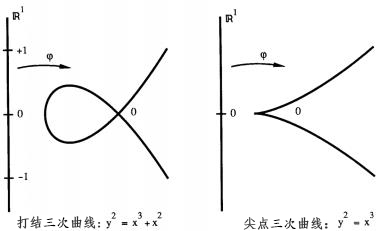
\includegraphics[width=10cm]{27.jpg} \\
		 % \caption{初}
		\end{figure}
		
		\textit{想想图像曲线和映射的奇点, 这些例子会贯穿整个课程, 所以花点时间来处理这些方程.}

	\section{曲线$(y^{2}=x(x-1)(x-\lambda))$没有有理参数化}
		参数化曲线很好; 例如, 如果您对丢番图问题感兴趣, 您可以期望一个表达式给出所有有理值点, 如(1.1)所示.(1.1)的参数化形式为$ x = f(t), y = g(t) $, 其中$ f $和$ g $是有理函数,即两个多项式的商.
		
		\textbf{定理} \ $ k $是一个特征不为2的域, $\lambda\in k$且$\lambda\neq0,1;f,g\in k(t)$是有理函数, 满足$f^{2}=g(g-1)(g-\lambda)$, 则$f,g\in k$.
		
		
		这相当于说不存在任何由有理函数给出的非常数映射$\mathbb{R}^{1}\rightarrow C: (y^{2}=x(x-1)(x-\lambda))$.
		
		
		定理的证明是在$ k(t) $中利用$ k(t) $是唯一分解整环$ k[t] $的分式域的事实.
		
		
		\textbf{证明} \ $ k[t] $是唯一分解整环, 设$f=r/s,  $ 其中 $r,s\in k[t]$且互素, $g=p/q, $ 其中 $ p,q\in k[t]$且互素, 代入 $f^{2}=g(g-1)(g-\lambda)$得
		$\dfrac{r^{2}}{s^{2}}=\dfrac{p}{q}(\dfrac{p}{q}-1)(\dfrac{p}{q}-\lambda)$, 除去公分母后得, $r^{2}q^{3}=s^{2}p(p-q)(p-\lambda q)$, 因为$ r $和$ s $是互素的, 右边的因子$s^{2}$一定整除$q^{3}$. 同理,因为$ p$ 和 $q $是互素的, 左边的因子$q^{3}$一定整除$s^{2}$.所以,$s^{2}|q^{3}$ 且$q^{3}|s^{2}$, 所以$s^{2}=aq^{3}$, 其中$a\in k$($ a $是$ k[t] $中的单位元,所以$a\in k$).
		
		
		可得$aq=(\dfrac{s}{q})^{2}$是$ k[t] $中的平方形式. 并且$r^{2}=ap(p-q)(p-\lambda q)$, 所以考虑分解到素元的因式分解, 存在非零常数$b,c,d\in k $ 使$bp,c(p-q),d(p-\lambda q)$是$ k[t] $中的平方形式. 下面如果能证明$ p, q $是常数, 那么$ r, s $也是, 定理得证. 为了证明$ p, q $是常数, 设$ K $是$ k $的代数闭包; 那么$p,q\in K[t]$满足以下引理的条件.

	\section{引理}
		K是一个代数闭域, $p,q\in K[t]$互素,假设4个不同的线性组合($\lambda p+\mu q$, 4个不同的比例$(\lambda:\mu)\in \mathbb{P}^{1}_{k}$)为$ K[t] $中的平方形式. 那么$p,q\in K$.
		
		
		\textbf{证明} \ (费马无穷递降法)不妨将$ p,q $替换成$ p'=ap+bq,q'=cp+dq $, 其中$a,b,c,d\in K$并且$ad-bc\neq 0$, 因此我可以假设4 个给定的平方形式是$p,p-q,p-\lambda q,q$. 那么$p=u^{2},q=v^{2}$, 并且$u,v\in K[t]$互素, 则$max\{deg\ u,deg\ v\}$小于$max\{deg\ p,deg\ q\}$. 假设$max\{deg\ p,deg\ q\}$大于0, 并且是满足引理条件的$ p,q $中次数最小的, 那么$p-q=u^{2}-v^{2}=(u-v)(u+v)$ 且$p-\lambda q=u^{2}-\lambda v^{2}=(u-\mu v)(u+\mu v)$(其中$\mu=\sqrt{\lambda}$)是$ K[t] $中的平方形式. 所以根据$ u,v $互素的形式,可得每个$u-v,u+v,u+\mu v,u-\mu v$都是平方形式. 这与$ max\{deg\ p,deg\ q\} $的极小性矛盾. 所以$max\{deg\ p,deg\ q\}=0, p,q\in K.$
	\section{线性系统}
		记$S_{d}$={$ (X,Y,Z) $的$ d $次型}(这个形式是齐次多项式),任意元素$F \in S_{d}$可以唯一地写成
		\begin{equation*}
		F=\sum a_{ijk} X^{i}Y^{j}Z^{k},\text{其中}a_{ijk} \in k,\text{且}i,j,k > 0,i+j+k=d
		\end{equation*}
		这意味着$S_{d}$是一个$ k $上的向量空间,它有基底
		\begin{center}
		$Z^{d}$\\
		$Z^{d-1}X  \quad Z^{d-1}Y$\\
		$ \cdots    \qquad        \cdots $\\
		$X^{d-1}Z  \quad X^{d-2}YZ  \cdots  \quad Y^{d-1}Z$\\
		$X^{d}\quad X^{d-1}Y  \quad X^{d-2}Y^{2}\quad   \cdots  \quad Y^{d}$\\
		\end{center}
		特别的,$dimS_{d}$=
		$\begin{pmatrix}
		     d+2  \\
		      2
		\end{pmatrix}$
		.对于$P_{1},...P_{n} \in \mathbb{P}^{2}$,令
		\begin{equation*}
		S_{d}(P_{1},..P_{n})=\{F\in S_{d}|F(P_{i})=0,\text{其中}i=1,2,...n\} \subset S_{d}
		\end{equation*}
		对于每个条件$ F(P_{i})=0 $,(或者更精确一点,$ F(X_{i},Y_{i},Z_{i})=0,P_{i}=(X_{i}:Y_{i}:Z_{i})) $
		是$ F $上的线性条件,因此$S_{d}(P_{1},..P_{n})$是一个维数$\geq\left(\begin{array}{c}{d+2} \\ {2}\end{array}\right)-n$的向量空间.
	\section{引理}
		设$ k $是一个无限域,$F \in S_{d}$.
		
		
		(i)记$L\subset \mathbb{P}^{2}_{k}$为一条直线,如果在$ L $上$F\equiv 0$,那么$ F $由$ L $的方程在$ k[X,Y,Z] $上是可分的.这是说,$ F=H·F' $成立,当$ H $是$ L $的方程且$F'\in S_{d-1}$
		
		
		(ii)记$C\subset \mathbb{P}^{2}_{k}$是一条非空非退化的圆锥曲线,如果在$ C $上$ F \equiv 0 $,,那么$ F $由$ C $的方程在$ k[X,Y,Z] $上是可分的.这是说,$ F=Q·F' $成立,当$ Q $是$ C $的方程且$F' \in S_{d-2}$.
		
		
		\textbf{证明}\ (i)通过坐标变换,我们可以假定$ H=X $,那么对于任意的$F \in S_{d}$,存在唯一一个表达式$F=X· F'_{d-1} +G(Y,Z)$:只需把所有含$ X $的单项式集中到第一个被加数里,剩下的就必然只有含$ Y,Z $的多项式.现在有在$ L $上$F \equiv 0 \Leftrightarrow$在$ L $上$G \equiv 0\Leftrightarrow G(Y,Z)=0$. 最后一步是由于(1.7):如果$ G(Y,Z) \ne 0 $,那么它在$\mathbb{P}^{1}_{k}$上至多有$ d $个零点,然而如果$ k $是无限域,那么对于$\mathbb{P}^{1}_{k}$也一样.
		
		
		(ii)通过坐标变换,$Q=XZ-Y^{2}$.现在证明对任意$F\in S_{d}$,都存在唯一一个表达式$ F=Q·F'_{d-2}+A(X,Z)+YB(X,Z) $:如果用$ (XZ-Q) $来代替$Y^{2}$,那么剩下的部分$ Y $的次数就一定不大于1,故是$ A(X,Z)+YB(X,Z) $的形式.正如在(1.8)中,$ C $是一个由$X=U^{2},Y=UV,Z=V^{2}$参数化的圆锥曲线,使得
		\begin{equation*}
		\begin{split}
		C\text{上}F\equiv0&\Leftrightarrow C\text{上}A(U^{2},V^{2})+UVB(U^{2},V^{2})\equiv0\\
		&\Leftrightarrow A(U^{2},V^{2})+UVB(U^{2},V^{2})=0\in k[U,V]\\
		&\Leftrightarrow A(X,Z)=B(X,Z)=0
		\end{split}
		\end{equation*}
		
		分开考虑$ A(U^{2},V^{2})+UVB(U^{2},V^{2}) $的奇次项和偶次项最后一个等式可以得到最后一个等式.证毕.
		
		\textbf{推论}\ 令$L:(H=0)\subset \mathbb{P}^{2}_{k}$为一条直线(另外的$C:(Q=0) \subset \mathbb{P}^{2}_{k}$是一条非退化圆锥曲线);假设给定点$P_{1},P_{2} ... P_{n} \in \mathbb{P}^{2}_{k}$,考虑$S_{d}(P_{1},P_{2} ... P_{n}),d$已给定.那么
		
		(i)如果$P_{1},P_{2} ... P_{a} \in L, P_{a+1},P_{a+2} ... P_{n} \notin L$,且$ a>d $,那么
		
		
		\quad $S_{d}(P_{1},P_{2} ... P_{n} )=H·S_{d-1}(P_{a+1},P_{a+2} ... P_{n})$
		
		(ii)如果$P_{1},P_{2} ... P_{a} \in C, P_{a+1},P_{a+2} ... P_{n} \notin C$,且$ a>2d $,那么
		
		
		\quad $S_{d}(P_{1},P_{2} ... P_{n} )=Q· S_{d-2}(P_{a+1},P_{a+2} ... P_{n})$
		
		
		\textbf{证明}\ 如果F是一个d次齐次多项式,曲线$ D:(F=0) $与$ L $相交于$P_{1}...P_{a}$当$ a>d $,那么由(1.9),就一定有$L\subset D$,因此由引理可知$ F=H·F^{\prime} $;由于$P_{a+1} ,...., P_{n} \notin L,$ 显然 $F^{\prime} \in S_{d-1}(P_{a+1} ... P_{n})$.同理可得(ii)的结论.证毕.
	\section{命题}
		令k是一个无限域,$P_{1} ... P_{8} \in \mathbb{P}^{2}_{k}$是两两不同的点,如果这8点中没有任意4点共线,而且没有任意7点在同一个非退化圆锥曲线上,那么
		\begin{equation*}
		dimS_{3}(P_{1}...P_{8})=2
		\end{equation*}
		
		
		\textbf{证明}\ (2.6)的证明分几种情况.
		
		
		\textbf{大多数情况}\ 没有任意3点共线,没有任意6点共圆锥曲线.这是一般的位置情况.
		
		
		假设$dim S_{3}(P_{1}...P_{8})\ge 3$,然后令$P_{9},P_{10}$是直线$L=P_{1} P_{2}$.那么
		\begin{equation*}
		dim S_{3}(P_{1}...P_{10})\ge dim S_{3}(P_{1} ... P_{8} )-2 \ge 1
		\end{equation*}
		
		
		所以有$0 \ne F \in S_{3} (P_{1} ... P_{10} )$.由推论$ 2.5 $,$F=H·Q,$ 其中 $Q \in S_{2} (P_{3} ... P_{8} )$.现在可以得出矛盾;如果$ Q $是非退化的那么$P_{3} ... P_{8}$是共圆锥曲线的,然而如果$ Q $是线对或二重线,那么它们中至少3点共线.
		\begin{figure}[H]
		  \centering
		  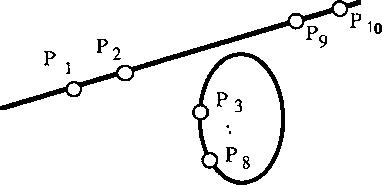
\includegraphics[width=8cm]{32.jpg}
		 % \caption{初}
		\end{figure}
	
	
		\textbf{第一退化情况}\ 设$P_{1} P_{2} P_{3} \in L$是共线的,令$ L:(H=0) $.令$P_{9}$是$ L $上的第四个点,那么由定理2.5,
		\begin{equation*}
		S_{3}(P_{1} ... P_{9} )=H· S_{2}(P_{4} ... P_{8} )
		\end{equation*}
		
		
		同样,由于$P_{4}...P_{8}$中不存在四点共线的,由1.11的推论,$dim S_{2}(P_{4} ... P_{8} )=1$,并且$dim S_{3}(P_{1} ... P_{9} )=1$,这意味着$dim S_{3}(P_{1} ... P_{8})\le 2$
		
		
		\textbf{第二退化情况}\ 设$P_{1} ... P_{6} \in C$是共圆锥曲线的,$ C:(Q=0) $是一个非退化圆锥曲线.那么选择区别于$P_{1} ... P_{6}$的$P_{9} \in C$,由推论2.5,
		\begin{equation*}
		S_{3}(P_{1} ... P_{9} )=Q· S_{1} (P_{7},P_{8} )
		\end{equation*}
	
	
		线$L= P_{7} P_{8}$是唯一的,所以$S_{3}(P_{1}...P_{9})$是由$ QL $限制的一维空间,因此$dim S_{3}(P_{1} ... P_{8})\le 2$.证毕.
	\section{推论}
		$C_{1} C_{2}$是两条三次曲线,它们的交点是9个两两不同的点,$C_{1} \cap C_{2} =\{ P_{1} ... P_{9} \}$.那么圆锥曲线$ D $如果通过$P_{1} ... P_{8}$,也必然穿过$P_{9}$.
		
		
		\textbf{证明}\ 如果$P_{1} ... P_{8}$中的4个点在一条线$ L $上,那么$C_{1}$ 和 $ C_{2}$都会与$ L $有4个以上交点,因此一定包含直线$ L $,这与$C_{1}\cap C_{2}$的假设矛盾.同样的,不能有7个点共圆锥曲线.因此满足了2.6的假设,所以
		\begin{equation*}
		dim S_{3}\left(P_{1} \ldots P_{8}\right)=2
		\end{equation*} 
		这意味着$C_{1},C_{2}$的等式$F_{1},F_{2}$构成了$S_{3}(P_{1} ... P_{8} )$的基.因此$ D:(G=0) $,其中G=$\lambda$$F_{1}$+$\mu$$F_{2}$.现在$F_{1}(P_{9}) = 0,F_{2}(P_{9}) = 0$,因此$ G $也一样.证毕.
	\section{平面三次曲线的群论}
		假设$ k \subset \mathbb{C} $是$ \mathbb{C} $的子域,$ F \in k[X,Y,Z] $是一个定义了一个非空平面曲线$ C $的三次型,$C:(F=0) \subset \mathbb{P}^{2}_{k}$.假定$ F $满足以下两条性质:
		
		
		(a)\ $ F $是不可约的(这样$ C $就不会包含一条直线或圆锥曲线);
		
		
		(b)\ 对于任意一点$ P \in C $,都存在唯一一条$L \subset \mathbb{P}^{2}_{k}$使得$ P $是$F|_{L}$的重根.
		
		
		几何上,条件(b)要求$ C $是非奇异的,$ L $指的是切线$L=T_{P} C$.
		
		
		固定任意一点$ O \in C $,进行下列构造:
		
		
		\textbf{构造}\ 
		\begin{minipage}[t]{0.9\linewidth}
			(i)对$ A \in C $,令$\overline{A}$为$ C $与$ OA $的第三个交点;\\
			(ii)对于$A,B\in$C,记$ R $为$ AB $与$ C $的第三个交点,并根据$A+B=\overline{R}$定义$ A+B $.
		\end{minipage}
		
		\textbf{定理}\ 上述构造在$ C $上定义了一个阿贝尔群,其中$ O $是零点(或者说是零元).
		
		\textbf{证明}\ 结合性是这里的关键.
		
		
		(I)需证明加法和逆运算是良定义的.如果$ P,Q $是$ C $上任意两点,那么$ P \ne Q $,这样$L=PQ\subset \mathbb{P}^{2}_{k}$是唯一确定的,不然由假设(b)知$ P=Q $,那么有唯一一条直线$L\subset \mathbb{P}^{2}_{k}$使得$ P $ 是$F|_{L}$的重根;在另一种情况下,$F|_{L}$是有两个变量的三次型,有两个$ k $上的零点.因此它分为3个线性因式的乘积,故无一例外的,第三个交点$ R $是良定义的而且在k内有坐标.注意$ P=Q,P=R,Q=R,P=Q=R $都是可以的.这在代数上与$F|_{L}$有多个零点一致,在几何上与切线和拐点一致.
		
		
		\begin{figure}[H]
		  \centering
		  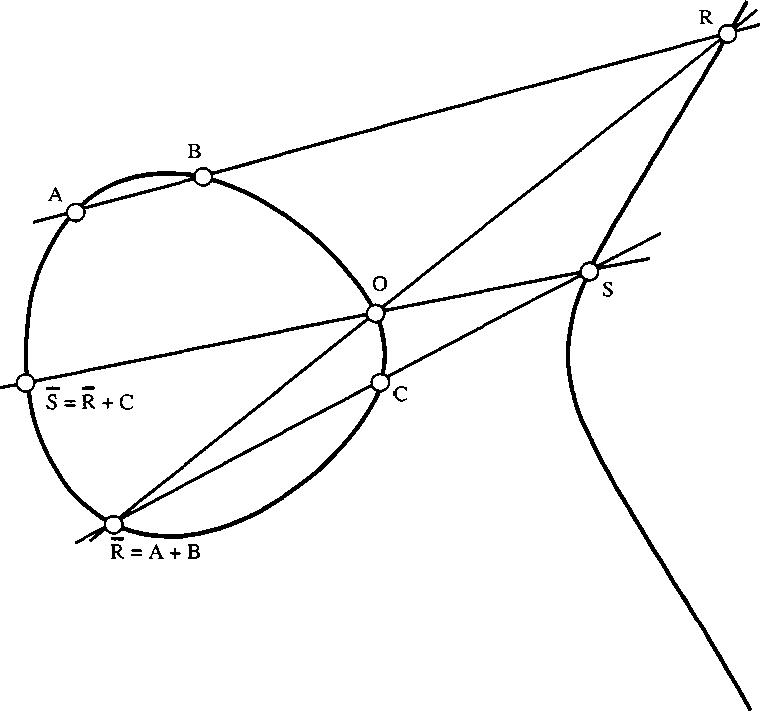
\includegraphics[width=10cm]{34.jpg}
		 % \caption{初}
		\end{figure}
		(II)验证零元$ O $点是符合零元条件的:$OA\overline{A}$是共线的,$ O+A $由$ L=OA $得到第三个交点$\overline{A}$,则根据同一条线$L=O\overline{A}$得到$ A $,得证.
		
		
		(III)$ A+B=B+A $显然.
		
			
		(IV)为了定义逆运算,先由构造(i)定义点$\overline{O}$:令$ L $为使得$ O $是$F|_{L}$重根的直线,定义$\overline{O}$是$ L $与$ C $的第三个交点.那么显然对任意$ A \in C $,$\overline{O} A$的第三个交点都是$ A  $的逆.
	\section{}
		现在,我们给出一个“足够普遍”的情况下的结合律的证明:假设$ A,B,C $是三次曲线$ C $上的三点,而$(A+B)+C=\overline{S}$的构造用到了四条直线(如上一节图):
		\begin{equation*}
			L_{1}:ABR,L_{2}:RO\overline{R},L_{3}:C\overline{R}S,L_{4}:SO\overline{S}
		\end{equation*}
	
		$(B+C)+A=\overline{T}$的构造则用到了另外四条直线:
		
		\begin{equation*}
			M_{1}:BCQ,M_{2}:QO\overline{Q},M_{3}:A\overline{Q}T,M_{4}:TO\overline{T}
		\end{equation*}
		我们需要证明$\overline{S}=\overline{T}$,显然,只需要证明$S=T$即可.考虑三次曲线:
		\begin{equation*}
		D_{1}=L_{1}+M_{2}+L_{3} \text { 和 }D_{2}=M_{1}+L_{2}+M_{3}
		\end{equation*}
		由构造可知,
		\begin{equation*}
		C \cap D_{1}=\{A, B, C, O,R, \overline{R}, Q, \overline{Q}, S\}
		\end{equation*}
		\begin{equation*}
		C \cap D_{2}=\{A, B, C, O,R, \overline{R}, Q, \overline{Q}, T\}
		\end{equation*}
		已知,$ A, B, C, O,R, \overline{R}, Q, \overline{Q}, S $这九个点都是独立的,三次曲线$ C $ 和 $ D_{1} $满足推论2.7的条件,因此,$ D_{2} $ 一定经过$ S $,而这当且仅当$S=T$时成立.
		
		
		完成这个证明有很多方法,其中最彻底的证明给出了考虑多交点的两条曲线的交点的真实处理方法,而对应推论2.7的证明是Max Noether的引理.
		
	\section{}
		在这里,我们给出一个利用连续性的证明,这个证明将用到$ k \in \mathbb{C} $这个事实.对曲线$ C $考虑对应的复曲线$C_{\mathbb{C}} \subset \mathbb{P}^{2}_\mathbb{C}$,即当$ (X:Y:Z) $在复数域上时仍然有$ F(X,Y,Z)=0 $.而如果结合律在复曲线$ C_{\mathbb{C}} $上成立,那么显然在曲线$ C $ 上也处处成立.因此,我们不妨假设$ k = \mathbb{C} $.
		
		\textbf{引理}\ (i)$ A+B $是对于$ A $和$ B $的连续函数.
		
		
		(ii)对于所有$ A,B,C \in C $存在任意近的三点$ A',B',C' \in C $使得构造出来的九点$ A', B', C', $  $O,R, \overline{R}, Q, \overline{Q}, S $都是独立的.
		
		
		加法$\varphi: C \times C \rightarrow C$是一个由$(A, B) \mapsto A+B$定义的映射.由(i),$ \varphi $是连续的,因此有两个映射$f=\varphi \circ(\varphi \times id_{C})$  和  $g=\varphi \circ(id_{C} \times \varphi): C \times C \times C \rightarrow C$分别由$(A, B,C) \mapsto (A+B)+C$和$ A+(B+C )$定义.并且,由(ii),能使这九个点的构造是独立的子集$ U \subset C \times C \times C  $由$ (A,B,C) $组成,并且是稠密的;由上面的证明,$ f $和$ g $在$ U $上总相等,则由连续性,它们处处相等.
		
		
		\textbf{注}\ 连续性的证明是建立在$ \mathbb{C} $的拓扑上的,因此这个证明不是纯代数的.事实上加法映射$ \varphi $是$\varphi: C \times C \rightarrow C$的一个态射,并且会在(4.14)证明,而剩下的部分可以重构成纯代数的形式:$ C \times C \times C $的能使这九个点的构造是独立的子集是Zariski拓扑上的稠密开集,而在稠密开集上相等的两个态射处处相等.
	\section{帕斯卡定理}
			图中是一个平	面$\mathbb{P}^{2}_{k}$中六边形$ ABCDEF $,它的对边延伸直至相交到点$ P,Q,R $. 假设这九个点和六条边都是不同的;则
			\begin{equation*}
				ABCDEF\text{共圆锥曲线} \Longleftrightarrow PQR\text{共线}
			\end{equation*}
		
			这个著名的定理是2.7的一个相当相似的应用,给出它只是为了好玩;当然其它证明也是有益的,在大多数的几何书上都有相关论证.
			\begin{figure}[h]
			  \centering
			  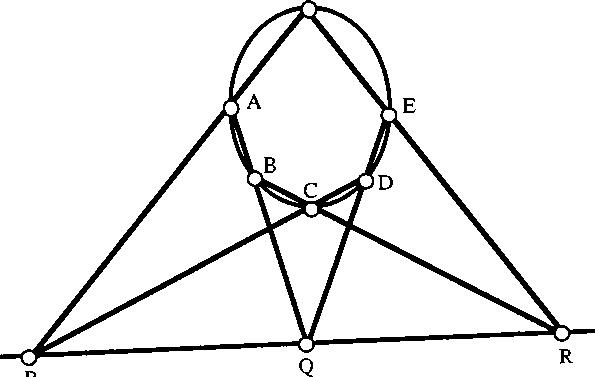
\includegraphics[width=10cm]{37.jpg}\\
			 % \caption{初}
			\end{figure}
		
		
			\textbf{证明} \ 在图中, 考虑两组直线
			\begin{equation*}
				L_{1}:PAF, L_{2}:QDE, L_{3}:RBC	
			\end{equation*}
			和
			\begin{equation*}
				M_{1}:PCD, M_{2}:QAB, M_{3}:REF	
			\end{equation*}
			令$C_{1}=L_{1}+L_{2}+L_{3},C_{2}=M_{1}+M_{2}+M_{3}$, 应用2.7,显然$C_{1}$和$C_{2}$是两条三次曲线且满足
			\begin{equation*}
			C_{1} \cap C_{2}=\{A,B,C,D,E,F,P,Q,R\}
			\end{equation*}
			假如$ PQR $共线, $ L=PQR $; 令$\Gamma$为过$ ABCDE $的圆锥曲线(其存在唯一性由推论1.11给出). 然后, 通过构造,$L+\Gamma$是一条通过8个点$ A,B,C,D,E,P,Q,R $的三次曲线, 则根据(2.7), 它一定通过点$ F $, 即$F \subset L \cup \Gamma$; 根据假设$F \notin L$, 所以$F \in \Gamma$, 故六点共圆锥曲线.
		
		
			反过来, 假设$ ABCDEF $在一个圆锥曲线$\Gamma$上, 令$ L=PQ $,则$L+\Gamma$是一个通过$ A,B,C,D,E,F,P,Q $的三次圆锥曲线,由2.7知,它一定通过$ R $. $ R $不可能在圆锥曲线$\Gamma$上(否则$\Gamma$是一对直线并且图中6条线中的一些会重合),所以$R\in L$, 即$ PQR $共线.
	\section{拐点, 标准形式}
		$\mathbb{P}^{2}_{\mathbb{R}}$或$\mathbb{P}^{2}_{\mathbb{C}}$中有能被写成标准形式
		\begin{equation*}
		C:Y^{2}Z=X^{3}+aXZ^{2}+bZ^{3}
		\end{equation*}
		或仿射形式
		\begin{equation*}
		C:y^{2}=x^{3}+ax+b
		\end{equation*}的曲线
	
		
		现在考虑上述曲线C; 它与无穷远直线$ L:(Z=0) $在何处相交?那很容易,只要把$ Z=0 $代入$F=-Y^{2}Z+X^{3}+aXZ^{2}+bZ^{3}$得到$F|_{L}=X^{3}$; 这意味着$F|_{L}=X^{3}$在$ P(0,1,0) $处有一个三重零点.
		
		为了看看这在几何上代表什么,令$ Y=1 $,得到$ (0,1,0) $附近关于仿射坐标$ (x,z) $的方程:
		\begin{equation*}
		z=x^{3}+axz^{2}+bz^{3}
		\end{equation*}
		这个曲线高度近似于$z=x^{3}$:
		
		
		\begin{figure}[h]
		  \centering
		  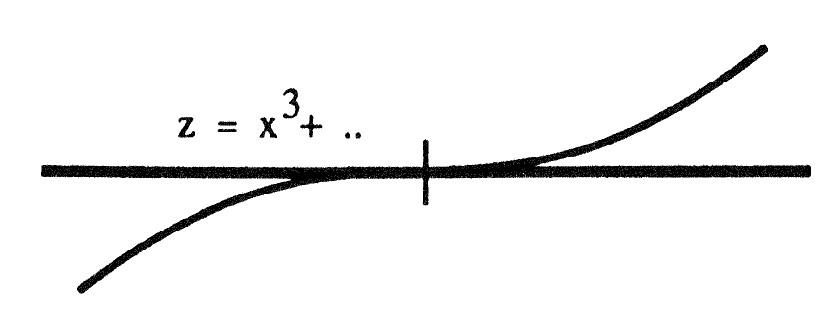
\includegraphics[width=5cm]{38.jpg}\\
		 % \caption{初}
		\end{figure}
	
	
	
		这说明$ C $在$ (0,1,0) $处有一个拐点.
		
		
		更一般地,$ C $上有一个拐点$ P $的定义是存在一条直线$L\subset \mathbb{P}^{2}_{k}$,使$F|_{L}$在$ P $点有一个 重数大于等于3 的零点(见习题2.9;事实上需要$L=T_{P}C(2.8,b)$且重数=3(1.9)), 不难用定义方程的导数和二阶导数来说明这一点, 如果定义方程是$ y=f(x) $, 那么$ P $为拐点的条件是,$\frac{d^{2}f}{dx^{2}(P)}=0$, 这在图中对应一个从凹向下到凹向上变化的曲线. 
		
		
		反过来(见\textit{习题2.10}),如果一条曲线$ C $有拐点,那么它的表达式一定能写成标准形式$C:Y^{2}Z=X^{3}+aXZ^{2}+bZ^{3}$.
	\section{简化的群}
		在标准形式
		$\mathbb{P}^{2}_{\mathbb{R}}$或$\mathbb{P}^{2}_{\mathbb{C}}$中有能被写成标准形式
		\begin{equation*}
		C:Y^{2}Z=X^{3}+aXZ^{2}+bZ^{3}
		\end{equation*}
		的曲线上定义群很方便:将点$ O(0,1,0) $作为零元. 在这些条件下,群的建立会很好,有以下几点原因:
		
		(a)$C=\{O\}\cup C_{0}:(y^{2}=x^{3}+ax+b)$, 所以可将曲线$ C $看作一条仿射曲线和无穷远一点O,即群的零元.
		
		(b)过O的直线是(2.8)(i)群的构造的主要部分,由$X=\lambda Z$给出,仿射坐标系中为$x=\lambda$; 这样的直线与C的交点或者是$(\lambda,\pm \sqrt{\lambda^{3}+a\lambda+b})$, 或者是无穷远点$ O $. 因此如果点$ P $的坐标为$ (x,y) $, 则(2.8,i)中构造的$\bar{P}$为$ (x,-y) $, 所以映射$P\mapsto\bar{P}$由 $(x,y)\mapsto(x,-y)$给出.
		
		\begin{figure}[h]
		  \centering
		  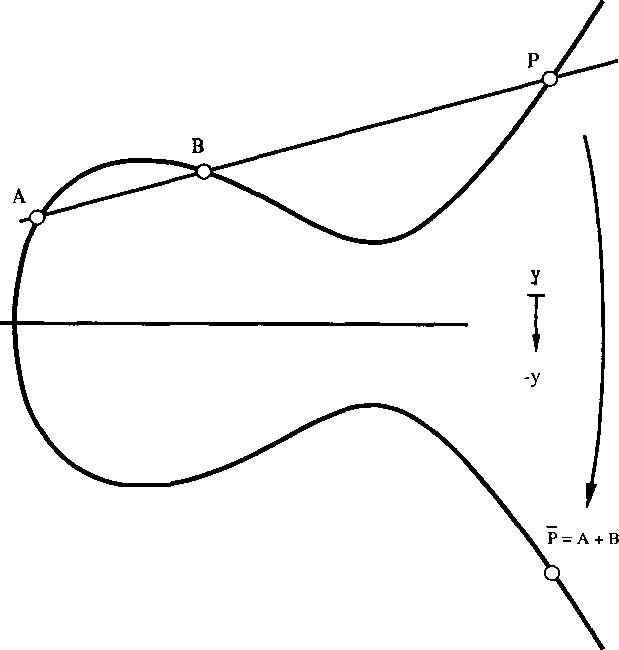
\includegraphics[width=5cm]{39.jpg}\\
		 % \caption{初}
		\end{figure}
	
	
	
		(c)由(2.8,IV),群的逆由$\bar{O}$给出,$\bar{O}$是以O为2重零点的直线L与C的第三个交点;在我们现在的情况下,这条直线是无穷远直线$ L:(Z=0) $且$L\cap C=3O$, 所以$\bar{O}=O$,群的逆简化为$-P=\bar{P}$.
		
		
		\textbf{定理} \ 
		$ C $是由标准形式$C:Y^{2}Z=X^{3}+aXZ^{2}+bZ^{3}$给出的一条三次曲线,那么在$ C $上有唯一的群使得$ O=(0,1,0) $是零元,元素的逆由由 $(x,y)\mapsto(x,-y)$给出, 且对任意的$P,Q,R\in C$,
		\begin{equation*}
			P+Q+R=O \Longleftrightarrow P,Q,R\text{共线}
		\end{equation*}
		
		
		\justifying	
		\textbf{证明} \ 左 $\Rightarrow$ 右 \   $P+Q=-R=\bar{R}$, 所以$ PQ $与$ C $的第三的交点为$ R $,即$ P,Q,R $共线.
		
		右$\Leftarrow$左 \ $P+Q=\bar{R}=-R$, 所以$ P+Q+R=O $.

		
		
\chapter{仿射簇和希尔伯特零点定理}
	前半部分大多是纯交换代数.在这一章中,环意味着有单位元的交换环.
	\section{命题与定义}
		下面的条件对于环$ A $来说等价.
		
		
		(i)每个理想$I \subset A$是有限生成的.即,任意理想$I \subset A$,存在$f_{1},...,f_{k} \in A$, 使得$I=(f_{1},...,f_{k}).$
		
		
		(ii)每一条$ A $的理想构成的升链
		
		
		\begin{equation*}
			I_{1} \subset ... \subset I_{m} \subset ...
		\end{equation*}
		
		
		会终止,即有$I_{N}=I_{N+1}=...$(升链条件,或简写为\textit{a.c.c}).
		
		(iii)$ A $的非空理想有极大元.
		
		
		若满足以上三个条件,则$ A $称为\textit{诺特环}.
		
		
		\textbf{证明}\ $(i) \Rightarrow (ii)$\ 假定$I_{1} \subset ... \subset I_{m} \subset ...$,设$I= \bigcup I_{m}$显然I仍为理想.如果$I=(f_{1},...,f_{k})$, 那么任意$f_{i}$都是$I_{m(i)}$的元素,所以取$m=max(m(i))$令$I=I_{m}$,则升链在此终止.
		
		
		$(ii) \Rightarrow (iii)$\ 由选择公理,显然成立.
		
		
		$(iii) \Rightarrow (i)$\ I为任意理想,记$\sum=\{J \subset I|J\text{是有限生成理想}\}$.由(iii),$\sum$有极大元,设为$J_{0}$.但是$J_{0}=I$,否则任意$f \in I\backslash J_{0}$可给出理想$J_{0}+Af$,它是有限生成的但比$J_{0}$大.
		
		
%		请证明$\mathbb{Z}$和$ k[X] $是诺特环.
		
	\section{命题}
		(i)$ A $为诺特环,$I \subset A$为理想,那么商环B=A/I为诺特环.
		
		
		(ii)令$ A $为诺特整环,$A \subset K$为分式域,$0 \notin S \subset A$是子集,令
		\begin{equation*}
			B=A[S^{-1}]=\{a/b \in K|a \in A,\text{且}b=1\text{或是$ S $中元素的乘积}\}
		\end{equation*}
		证明参考3.4.
		
		
	\section{希尔伯特基定理}
		环$ A $有,
		
		
		\begin{center}
			$ A $是诺特环$\Rightarrow A[X]$是诺特环.
		\end{center}
		
		
		\textbf{证明}\ 令$J \subset A[X]$是任意理想,证明$ J $有限生成.定义$ J $中首项为$ n $次的元素为
		
		
		\begin{center}
			$J_{n}=\{a\in A|\exists f=aX^{n}+b_{n-1}X^{n-1}+..+b_{0}\in J\}$.
		\end{center}
		
		
		那么$J_{n}$是A的理想而且$J_{n} \subset J_{n+1}$.因此,由升链条件,存在$ N $使$J_{N}=J_{N+1}=...$.
		
		
		建立J的生成元集:对于$i \leqslant N$,令$a_{i1},...,a_{im(i)}$为$J_{i}$的生成元,在$J_{i}$的定义里,对每个$a_{ik}$,令$f_{ik}=a_{ik}X^{i}+...\in J$为i次首项为$a_{ik}$的元素.
		
		
		下证集
		\begin{equation*}
			\{f_{ik}|i=0,...,N,k=1,...,m(i)\}
		\end{equation*}
		生成J:对给定的$g\in J$,假定$ deg g = m $.那么$ g $的首项为$bX_{m}$,$b\in J_{m}$.有$b=\sum c_{m'k}a_{m'k}($ 这里 $m'=m$ 若 $m\leqslant N,$ 否则 $m'=N)$.然后考虑$g_{1}=g-X^{(m-m')} \sum c_{m'k}f_{m'k}$:通过构造可使m次数为0,所以$deg\ g_{1} \leqslant deg\ g-1$;最终可写出$ g $由$f_{ik}$组合而成的形式,所以生成$ J $.
		
		
		\textbf{推论}\ 若$ k $为域,那么有限生成$ k $代数为诺特环.
		
		
		有限生成$ k $代数是一个形如$A=k[a_{1},...,a_{n}]$的环,所以$ A $是由$ k $与$a_{1},...,a_{n}$有限生成的环.很明显,每个这样的环都同构于一个多项式环的商环,$A \cong k[a_{1},...,a_{n}]/I$.一个域是诺特环,由(3.3),$k[a_{1},...,a_{n}]$是诺特环,最后由(3.2)(i)商环也是诺特环.
		
		
	\section{对应$ V $}
		$ k $是任意域,$A=k[X_{1},...,X_{n}]$.记$\mathbb{A}^{n}_{k}=k^{n}$为$ k $上$ n $维仿射平面.给出多项式$k(X_{1},...,X_{n})\in A$和点$P=(a_{1},...,a_{n}) \in \mathbb{A}^{n}_{k}=k_{n}$,则$f(a_{1},...,a_{n}) \in k$可以作为函数$ f $在$ P $上的估计.定义对应V
		
		\begin{center}
		$\{\text { 理想 } J \subset A \} \stackrel{ V }{\longrightarrow} \quad\left\{\text {子集 } X \subset \mathbb{A} ^{ n }_{ k }\right\}$
		\end{center}
		
		其中
		\begin{center}
		\qquad\qquad\qquad\qquad$J\qquad \mapsto \qquad V(J)=\left\{P \in \mathbb{A} ^{n}_{k} | f(P)=0 ,\forall f \in J\right\}$
	\end{center}
		\textbf{定义}\ 子集$X \subset \mathbb{A}^{n}_{k}$是代数集如果X=V(I)对某些I成立.由推论3.3,$ I $是有限生成的.如果$I=(f_{1},...,f_{r})$那么显然
		
		
		\begin{center}
			$V(I)=\{P \in \mathbb{A}^{n}_{k}|f_{i}(P)=0,\text{其中}i=1,..,r\}$
		\end{center}
		
		
		所以代数集是那些满足有限个多项式方程的点的轨迹.
		
		
		若$ I=(f) $是主理想,那么通常把$ V(I) $写成$ V(f) $.
		
		
	\section{命题与定义}
		对应$ V $满足:
		
		
		$(i)V (0)=\mathbb{A}^{n}_{k}; V(A)=\varnothing$;
		
		
		$(ii)I \subset J \Rightarrow V(I)\supset V(J)$;
		
		
		$(iii)V(I_{1} \bigcap I_{2}) = V(I_{1}) \bigcup (I_{2})$;
		
		
		$(iv)V(\sum _{\lambda \in \Lambda}I_{\lambda})=\bigcap _{\lambda \in \Lambda}V(I_{\lambda})$
		
		
		因此$\mathbb{A}^{n}_{k}$的代数集构成了$\mathbb{A}^{n}_{k}$上Zariski拓扑的闭集.
		
		
		只给出(iii)的$\subset$的证明.设$P\notin V(I_{1}) \bigcup V(I_{2})$,有$f\in I_{1},g\in I_{2}$使得$f(P) \ne 0,g(P) \ne 0$.所以$fg\in I_{1} \bigcap I_{2}$,但$fg(P) \ne 0$,因此$P\notin V(I_{1} \bigcap I_{2})$.
		
		
	\section{对应$ I $}
		对应$ I $是对应$ V $的某种逆
		
		
		\begin{center}
			$\{\text{理想}J\subset A\}\stackrel{I}{\longleftarrow} \{\text{子集}X \subset \mathbb{A}^{n}_{k}\}$
		\end{center}
		其中
			\begin{center}
			$I(X)=\{f \in A|f(P)=0,\forall P\in X\} \gets X$
		\end{center}
		
		
		这意味着$ I $把子集$ X $映成在$ X $上取0值的函数的理想.
		
		
		\textbf{命题}\ (a)$X\subset Y \Rightarrow I(X) \supset I(Y)$;
		
		
		(b)对任意子集$X \subset \mathbb{A}^{n}_{k}$,有$X \subset V(I(X))$;当且仅当X为代数集时$X = V(I(X))$;
		
		
		(c)对$J \subset A$,严格地有$J \subset I(V(J))$.
		
		
		$\textbf{证明}$\ (a)是显然的.(b)与(c)是对等相反的:若$ I(X) $被定义为在$ X $上所有点的值为$ 0 $的函数集,那么对于$ X $中任一点,所有$ I(X) $中函数在这一点的值为$ 0 $.
		
		
		(b)中剩下的部分很简单:若$ X=V(I(X)) $那么$ X $是代数集,因为它具有形式$ V $(是某一个理想).相反地,如果$X=V(I_{0})$是代数集,那么$ I(X) $至少包含$I_{0}$,故$V(I(X))\subset V(I_{0})=X$.
		
		
		有两种可能使(c)中的包含为严格的.
		
		
		\textbf{例1}\ 假设域$ k $不是代数闭的,令$f\in k[X]$为一个非常数多项式,且在$ k $中没有根.考虑理想$J=(f)\subset k[X]$.那么$J\ne k[X]$,因为$1\notin J$.但
		
		
		\begin{center}
			$V(J)=\{P\in \mathbb{A}^{1}_{k}|f(P)=0=\varnothing\}$
		\end{center}
		
		
		因此$ I(V(J))=k[X] $.
		
		
		所以如果域不是代数闭的,可能无法有足够的零点.一个相似的例子:在$\mathbb{R}^{2}$上,多项式$X^{2}+Y^{2}$定义了单点$P=(0,0)$,故$V(X^{2}+Y^{2})=\{P\}$.但是除此之外还有很多在$ \{P\} $上值为$ 0 $的多项式,而且事实上$ I(P)=(X,Y) $.
		
		
		\textbf{例2}\ 对任何$f\in k[X_{1},...X_{n}]$且$a\geqslant 2$,$f^{a}$定义了与$ f $相同的轨迹,$f^{a}(P)=0\iff f(P)=0$.所以$V(f^{a})=V(f)$,且$f\in I(V(f^{a}))$,但是通常$f\notin (f^{a})$.在\textbf{例1}中,讨论的是$X^{2}=0$定义的两条直线,它只表示(X=0)中的平方项,但事实并非如此.
		
		
	\section{不可约代数集}
		一个代数集$X\subset \mathbb{A}^{n}_{k}$是不可约的,如果不存在分解
		
		
		\begin{center}
			$X=X_{1}\cup X_{2}$ 其中 $X_{1},X_{2}\varsubsetneq X$
		\end{center}
		
		
		比如,代数集$V(xy)\subset \mathbb{A}^{n}_{k}$是由两坐标轴组成的轨迹,显然是$ V(x) $与$ V(y) $的组合,所以是可约的.
		
		
		$\textbf{命题}$\ (a)令$X\subset \mathbb{A}^{n}_{k}$是代数集且$ I(X) $是对应的理想.那么
		
		
		\begin{center}
			$ X $是不可约的 $\iff I(X)$是素理想.
		\end{center}
		
		
		(b)任何代数集$ X $有唯一分解
		
		
		\begin{center}
			$X=X_{1}\cup...\cup X_{r}$ 
		\end{center}
		
		
		其中$X_{i}$不可约且当$i\ne j$时$X_{i}\nsubseteq X_{j}$.同时,这些$X_{i}$被称作$ X $的不可约成分.
		
		
		\textbf{证明}\ (a)要证$ X $是不可约的$\iff I(X)$不是素的.
		
		
		$(\Rightarrow)$设$X=X_{1} \cup X_{2}$,其中$X_{1}\nsubseteq X$.其中$X_{1}\varsubsetneq X$意味着有$f_{1}\in I(X_{1})\backslash I(X)$,相似地$X_{2}\varsubsetneq X$ 意味着有$f_{2}\in I(X_{2})\backslash I(X)$.则乘积$f_{1}f_{2}$在$ X $的所有点上为取值为$ 0 $,故$f_{1}f_{2}\in I(X)$.则$ I(X) $不是素的.
		
		
		$(\Leftarrow)$设$ I(X) $不是素的,则有$f_{1},f_{2}\notin I(X)$使$f_{1}f_{2}\in I(X)$.取$I_{1}=(I(X),f_{1})$且$V(I_{1})=X_{1}$,那么$ X \varsubsetneq X_{1}$为代数集.同理,得到$X_{2}$. 由$X\subset X_{1}\cup X_{2}$,对任意$P\in X$,$f_{1}f_{2}(P)=0$意味着$f_{1}(P)=0$或$f_{2}(P)=0$.
		
		
		(b)$\mathbb{A}^{n}_{k}$中代数集满足降链条件,即
		
		
		\begin{center}
			$X_{1}\supset X_{2}\supset ... \supset X_{n} \supset...$
		\end{center}
		
		
		最终终止.这是因为
		
		
		\begin{center}
			$I(X_{1})\subset I(X_{2})\subset ... \subset I(X_{n}) \subset...$
		\end{center}
		
		
		是$ A $的理想构成的升链并且最终终止.正如在3.1中,
		
		
		\begin{center}
			$\mathbb{A}^{n}_{k}$上代数集的任何非空集合$\sum$有极小元.
		\end{center}
		
		
		令$\sum$为$\mathbb{A}^{n}_{k}$的代数子集,它没有唯一分解.若$\sum=\varnothing $那么(b)成立,否则,必有极小元$X\in \sum$,并且有矛盾:若$ X $不可约,那么$X\notin \sum$,矛盾;若X可约,那么$X= X_{1}\cup X_{2}$,其中$X_{1},X_{2}$为$ X $的真子集.又$ X $为极小元,$X_{1},X_{2}\varsubsetneq \sum$.所以$X_{1},X_{2}$各有唯一分解,把它们合并同样有唯一分解,故$X\notin \sum$.所以$\sum =\varnothing$.唯一性的证明是简单的,见\textit{习题3.8}.综上则(b)得证.
	\section{断言}
		让$ k $为(有限)域,$A=k[a_{1},...,a_{n}]$是有限生成$ k $代数.那么
		
		
		\begin{center}
			$ A $是一个域 $\Rightarrow$ $ A $在$ k $上是代数的
		\end{center}
		
		
		\textbf{提示}\ 若$t\in A$是$ k $上超越元,那么$ k[t] $是多项式环,有无限多个素元.因此扩张$k\subset k(t)$不是有限生成的$ k $代数:有限多个元素$p_{i}/q_{i}\in k(t)$只能有有限多个素的生成元.
		
		
	\section{定义}
		如果$ I $是$ A $的一个理想,那么$ I $的根是:
		\begin{equation*}
			rad I =\sqrt{ I }=\left\{ f \in A | f ^{ n } \in I \text {对于某些} n \right\}
		\end{equation*}
		$ rad I  $是一个理想,因为对于合适的$ n,m $有$f, g \in rad I \Rightarrow f^{n}, g^{m} \in I $ 并且因此
		\begin{equation*}
			( f + g )^{ r }=\sum\left(\begin{array}{l}{ r } \\ { a }\end{array}\right) f^{a}g^{r - a} \in I \text {如果} r \geq n + m -1
		\end{equation*}
		如果有 $I= rad I$,则称$ I $是一个根理想.
		
		
		 注意到,素理想都是根理想.显然,对于唯一分解整环例如$k \left[ X _{1}, \ldots X _{ n }\right],$ 一个主理想 $I =( f )$ 其中$f =\prod f _{ i }^{ n _{ i }}$ (分解成不同的主因子), 有$rad I=\left( f _{ red }\right),$ 其中$f _{ red }=\prod f _{ i }$
	
	
	
	\section{希尔伯特零点定理}
		假设$ k $是一个代数闭域.
		\begin{enumerate}[(a)]
			\item 多项式环$A=k \left[X_{1}, \dots X_{n}\right]$中的极大理想总是有着$m_{P}=\left(X_{1}-a_{1}, \ldots X_{n}-a_{n}\right)$的形式,其中$P=\left(a_{1}, \ldots a_{n}\right) \in \mathbb{A}^{n}_{k}$;也就是说,极大理想是在$ P $处取0值的所有函数的理想$ I(P) $.
			\item 如果$J \subset A$是一个理想,$J \neq(1)$,则$V (J ) \neq \varnothing$.
			\item 对于任意$J \subset A$,$ I(V(J)) = rad J$
		\end{enumerate}
		定理的必要条件是$ (b) $,即如果一个理想$ J $不是整个环$ k \left[X_{1}, \dots X_{n}\right] $,则理想中的多项式就会在$ \mathbb{A}^{n}_{k} $上有零点.注意,如果$ k $不是代数闭域,那么$   (b) $就是完全错误的,因为如果$f \in k [ X ]$是一个非常数多项式,那么$ f $就不能作为一个理想来生成整个$ k [ X ] $,但是可能有$ V(f) = \varnothing \subset \mathbb{A}^{1}_{k} $.
		
		
		\textbf{推论}\ 对应关系$ V $和$ I $
		
		
		\centerline{$\{\text { 理想 } I \subset A \}\quad{\stackrel{ V , I }{\longleftrightarrow}} \quad\left\{\text {子集} X \subset A ^{ n } k \right\}$}
		
		
		导出双射$ \qquad\qquad\qquad\qquad\quad\cup\qquad\qquad\qquad\qquad\qquad\cup $
		

		\centerline{\{根理想\} \qquad $\longleftrightarrow$ \qquad \{代数子集\}}
		
		
		以及$ \qquad\qquad\qquad\qquad\qquad\quad\cup\qquad\qquad\qquad\qquad\qquad\cup $
		
		
		\centerline{\qquad\quad \{素理想\} \qquad $\longleftrightarrow$ \qquad \{不可约代数子集\}}
		
		
		上述双射成立时因为由(3.6, b)对任意代数集$ X $有$ V(I(X))  = X$,而由(3.10, c)对任意根理想$ J $有$ I(V(J))  = J$.
		
		
		\textbf{零点定理的证明(假设3.8成立)}
		
		
		$ (a) $\ 设$m \subset k \left[ X _{1}, \ldots X _{ n }\right]$是一个极大理想,取$K = k \left[ X _{1}, \ldots X _{ n }\right] / m$,则有$ \varphi $是两个自然映射的合成$ \varphi : k \to k \left[ X _{1}, \ldots X _{ n }\right] \to K$.则$ K $是一个域(因为$ m $是极大的),而作为$ k $-代数$ K $是有限生成的(因为$ K $由$ X_{i} $的象生成).所以由(3.8),$ \varphi : k \to K $是一个代数的域扩张.但是$ k $是代数闭域,所以$ \varphi $是一个同构.
		
		
		现在,对每一个$ i $,$X _{ i } \in k \left[ X _{1}, \ldots X _{ n }\right]$映到一些元素$ b_{i} \in K$,所以取$a _{ i =} \varphi^{-1}\left(b _{ i }\right)$则有$X _{ i }- a _{ i } \in \operatorname{Ker}\left\{ k \left[ X _{1}, \ldots X _{ n }\right] \rightarrow K \right\}= m .$因此这里存在$a _{1}, \ldots a _{ n } \in k$使得$\left(X _{1}- a _{1}, \ldots X _{ n }- a _{ n }\right) \subset m .$另一方面,左侧显然是一个极大理想,因此$\left(X _{1}- a _{1}, \ldots X _{ N }- a _{ n }\right)= m .$则$ (a) $得证.
		
		
		$ (a)  \Rightarrow (b) $\ 这一部分证明是简单的.如果$J \neq A = k \left[ X _{1}, \ldots X _{ n }\right]$,那么对$ A $一定存在一个极大理想$m$使得 $J \subset m$ ($ m $的存在性是显然的,可以利用升链条件).由$ (a) $,$ m $具有形式$m =\left(X _{1}- a _{1}, \ldots X _{ n }- a _{ n }\right)$,则 $J \subset m$ 意味着对于任意 $f \in J$有$f (P )=0$ ,其中$P =\left(a _{1}, \ldots a _{ n }\right) .$因此$P \in V (J )$.
		
		
		$ (b)  \Rightarrow (c) $\ 这一部分需要一个小技巧.设$J \subset k \left[ X _{1}, \ldots X _{ n }\right]$是任意理想,而$f \in k \left[ X _{1}, \ldots X _{ n }\right]$.引入另外一个变量$ Y $,考虑由$ J $和$ fY - 1 $生成的新理想
		\begin{equation*}
		J _{1}=(J , f Y -1) \subset k \left[ X _{1}, \ldots X _{ n }, Y \right]
		\end{equation*}
		粗略地说,$ V(J_{1}) $是一个包含$ P \subset V(J) $的簇,因此$ f(P) \neq 0 $.更准确地说,一点$Q \in V\left(J_{1}\right) \subset \mathbb{A}^{n+1}_{k}$是一个$ n +1 $元$Q =\left(a _{1}, \ldots a _{ n },b \right)$使得
		\begin{equation*}
		\text {对所有} g \in J \text{有}g\left(a_{1}, \dots a_{n}\right)=0 , \text { 即} P=\left(a_{1}, \dots a_{n}\right) \in V(J)
		\end{equation*}
		以及
		\begin{equation*}
		f(P) \cdots b=1, \text {即} f(P) \neq 0 \text { 且 } b=f(P)^{-1}.
		\end{equation*}
		
		
		现在假设对所有$ P \in V(J) $有$ f(P) = 0 $,则显然由上文可得$ V(J_{1}) = \varnothing $.因此由$ (b) $可推出$ 1 \in J_{1}$,即存在表示
		\begin{equation*}
		\left.1=\sum g_{i} f_{i}+g_{0}(f Y-1) \in k | X_{1}, \ldots X_{n}, Y\right]
		\end{equation*}
		其中$ f_{i} \in J $而$ g_{0},g_{i} \in k \left[ X _{1}, \ldots X _{ n }, Y \right] $.
		
		
		考虑为什么上式中$ Y $在右侧:除了显式地表示,$ Y $还存在在每一个$ g_{i} $中,假设$ Y^{N} $是$ Y $在$ g_{0},g{i} $中存在的最高阶.如果将两边同乘$ f^{N} $,就有关系
		\begin{equation*}
		f ^{ N }=\sum G _{ i }\left(X _{1}, \ldots X _{ n }, f Y \right) f _{ i }+ G _{0}\left(X _{1}, \ldots X _{ n }, fY \right)(fY -1)
		\end{equation*}
		其中$ G_{i} $是$ f^{N}g_{i} $用$ X _{1}, \ldots X _{ n } $和$ (fY) $的多项式形式写出来的.
		
		
		上式是仅关于$ k \left[ X _{1}, \ldots X _{ n }, Y \right] $的多项式的等式,因此可以两边同模$ (fY -1) $得到
		\begin{equation*}
		f ^{ N }=\sum h _{ i }\left(X _{1}, \ldots X _{ n }\right) f _{ i } \in k \left[ X_{1}, \ldots X _{ n }, Y \right] /(f Y -1)
		\end{equation*}
		等式两边都是$ k \left[ X _{1}, \ldots X _{ n }\right] $中的元素.因此自然的同态$ k \left[ X _{1}, \ldots X _{ n }\right] \hookrightarrow k \left[ X _{1}, \ldots X _{ n }, Y \right] /(f Y -1)$是一个内射(这是$ k \left[ X _{1}, \ldots X _{ n }\right] $到$ k \left[ X _{1}, \ldots X _{ n }\right][f^{-1}] $的一个自然嵌入,就像子环和它的分式域一样),它遵循
		\begin{equation*}
		f ^{ N }=\sum h _{ i }\left(X _{1}, \ldots X _{ n }\right) f _{ i } \in k \left[ X _{1}, \ldots X _{ n }\right]
		\end{equation*}
		即对某些$ N $有$ f^{N} \in J $.则证毕.
		
		
	\section{一些实例}
		\textbf{(a)超曲面}
		
		
		关于簇的一个最简单实例是超曲面$V (f ):(f =0) \subset \mathbb{A} ^{ n } k$.如果$ k $是代数闭域,那么在不可约元$f \in k \left[ X _{1}, \dots X _{ n }\right]$和不可约超曲面上就有一个自然的对应关系:由零点定理,两个互质的不可约多项式$ f_{1},f_{2} $定义了两个不同的超曲面$ V(f_{1}),V(f_{2}) $.这并不总是显然的(例如,在$ \mathbb{R} $上就不成立),尽管这不用零点定理而用消去定理(19世纪提出的一个更加显式的方法)就能证明,即\textit{练习3.13}.
		
		
		\textbf{(b)}
		
		
		除了超曲面外,绝大多数的簇都是由很多等式来定义的.反直觉地,这通常都是因为理想$ I(X) $有多个生成元,即多于$ X $的共同维数的生成元.例如,对于$C \subset \mathbb{A} ^{3} _{k}$,$ I(C) $需要三个生成元,现在假设$ k $是一个无限域.
		
		
		先考虑,$J =\left(uw - v ^{2}, u ^{3}- vw \right)$.其中$ J$不是素的,因为
		\begin{equation*}
		 J \ni w \left(uw - v ^{2}\right)- v \left(u ^{3}- v w \right)= u \left(w ^{2}- u ^{2} v \right)
		\end{equation*}
		 而$ u , w ^{2}- u ^{2} v \notin J $.因此
		 \begin{equation*}
		 	V (J )= V (J , u ) \cup V \left(J , w ^{2}- u ^{2} v \right)
		 \end{equation*}
		 显然,$ V (J , u ) $是直线$ (u = v =0) $.同时,另外一部分$  C = V \left(J , w ^{2}- u ^{2} v \right)$是一个不可约曲线,而$ C $由三部分给出:
		 \begin{equation*}
		 	uw = v ^{2}, u ^{3}= vw , w ^{2}= u ^{2} v
		 \end{equation*}
		
		
		现在证明$C \subset \mathbb{A} ^{3}$是映射$\varphi: \mathbb{A} ^{1} \rightarrow C \subset A ^{3}$在$t \mapsto t^{3}, t^{4}, t^{5}$下的象:如果$u \neq 0$ 则 $v, w \neq 0 .$取$t=v / u,$ 则$t=w / v $ 且 $t ^{2}=(v / u )(w / v )= w / u .$因此$v = w ^{2} / u ^{2}= t ^{4}, u = v /(v / u )= t ^{4} / t = t ^{3} $ 并且
		$w = tv = t ^{5},$ 则 $C$ 是不可约的, 因此如果$C = X _{1} \cup X _{2}, X _{ i } \subset C ,$ 且 $f _{ i }(u , y , w ) \in I \left(X _{ i }\right),$则对于所有 $t ,$ 至少有一个 $f _{ i }\left(t ^{3}, t ^{4}, t ^{5}\right)$取到0值. 因为一个非零多项式至多有有限个零点, $f_{1}, f_{2}$中的一个必须为0,所以$f _{ i } \in I (C )$.
		
		
		这个实例是一个不错的单项式的例子,通常情况下是很难找到一个簇的不可约部分的,更别提证明它不可约了.一个同样的例子为\textit{练习 3.11}
		
		
	\section{有限代数}
		现在开始证明$ (3.8) $.设$A \subset B$都是环.通常来说,如果存在有限个元素$b_{1}, \dots b_{n}$使得$B=A\left[b_{1}, \ldots b_{n}\right],$则$ B $被称作在$ A $上的有限扩张(或$ A- $代数),因此$ B$由$ A $和$b_{1}, \ldots b_{n}$生成.
		
		
		与下述定义做对比:如果存在有限个元素$b_{1}, \dots b_{n}$使得$B=A b_{1}+. . A b_{n},$则$ B $被称作有限$ A- $代数,即,$ B $作为$ A- $模是有限生成的.
		
		
		两个定义最大的不同是一个是作为环(即允许对$ b_{i} $的任意多项式表达),一个是作为模(只允许线性表达).例如,$ k[X] $是一个有限生成$ k- $代数(仅由一个元素$ X $生成),但这不是一个有限$ k- $代数(因为作为$ k- $向量空间它是无限维的).
		
		
		\textbf{命题}\  (i)设 $A \subset B \subset C$都是环: 则
		
		\begin{equation*}
		\begin{split}
		B\text{是有限} A -\text{代数且}&C \text{是有限} B -\text{代数}\\
		\Rightarrow &C \text {是有限 }A -\text{代数}
		\end{split}
		\end{equation*}
		
		
		(ii) 如果$A \subset B$是一个有限$ A $-代数且 $x \in B$则$x$满足一个在$A$上的首一多项式,即存在关系
		\begin{equation*}
		x^{n}+a_{n-1} x^{n-1}+. . a_{0}=0 \text {其中}a_{i} \in A
		\end{equation*}
		(注意其中首项系数是1).
		
		
		(iii) 反过来,如果$x$满足一个在$A$上的首一多项式,则$B=A[x]$ 是一个有限$ A- $代数.
		
		
		\textbf{证明}\  (i)和(iii)简单的(仿照域扩张的相似结论). 对于(ii),可以使用一个不太显然的行列式技巧:假设$B =\sum A b _{ i } ;$ 则对于任意$i ,  x b_{ i } \in B ,$ 所以有常数$a_ij \in A$使得
		\begin{equation*}
		x b_{i}=\sum_{j} a_{i j} b_{j}
		\end{equation*}
		
		
		也可以写作
		\begin{equation*}
		\sum_{j}\left(x \delta_{i j}-a_{i j}\right) b_{j}=0
		\end{equation*}
		其中$\delta_{ ij }$是单位矩阵.则设$M$是矩阵:
		
		\begin{equation*}
		M _{ i j }=\left(x \delta_{ i j }- a _{ i j }\right)
		\end{equation*}
		
		然后取$\Delta=\operatorname{det} M .$ 然后由标准线性代数, (将$b$写作列向量和项$\left(b_{1}, \dots b_{n}\right)$ 以及$M$的伴随矩阵 $M^adj$).
		\begin{equation*}
		Mb =0, \quad \text { 因此 } \quad 0=\left(M ^{ adj }\right) Mb =\Delta b
		\end{equation*}
		则对所有$ i $有$\Delta b_{i}=0$. 但是, $1_{B} \in B$是关于 $b _{ i }$的线性组合,因此 $\Delta=\Delta \cdots 1 B =0,$最后则得到关系: $\operatorname{det}\left(x \delta_{ ij }- a _{ ij }\right)=0 .$ 则显然有对$x$的首一多项式,而系数则来自$ A $.
		
		
	\section{诺特正规化}
		\textbf{诺特正规化引理}\ 设$k$ 是一个无限域, 同时$A=k\left[a_{1}, \ldots a_{n}\right]$是一个有限生成的$k$ -代数. 则存在$m \leq n$和$y_{1}, . . y_{m} \in A$使得
		\begin{enumerate}[(i)]
			\item  $y _{1} \ldots y _{ m }$ 在$k$上代数独立;
			\item $A$是有限$k \left[ y _{1}, \dots y _{ m }\right]$ -代数.
		\end{enumerate}
		
		
		((i)意味着对$y_{i}$的线性组合,当且仅当系数全为0时才取到0值; 代数地来讲,就是自然的映射$k \left[ Y _{1}, \ldots Y _{ m }\right] \rightarrow k \left[ y _{1}, \ldots y _{ m }\right] \subset A$是单射.
		
		可以断言,环的扩张可以通过首先引入代数独立的元素,然后“进行代数扩张”来建立.但是,(ii)远比此精确得多,因为它说$ A $中的每个元素不仅是在$ k \left [y _ {1},\ldots y _ {m} \right]$上代数的,还满足在其上的首一多项式.
		
		
		
		\textbf{证明}\ 取$ I $是自然满射的核
		\begin{equation*}
		I =\operatorname{ker}\left\{ k \left[ X _{1}, \ldots X _{ n }\right] \rightarrow k \left[ a _{1}, \ldots, a _{n}\right]= A \right\}
		\end{equation*}
		假设$0 \neq f \in I ;$ 证明的思路是将$X _{1} \ldots X _{ n -1}$ 替换为确定的$X _{1}^{\prime} \ldots X _{ n -1}^{\prime}$使得$f$对于$a _{ n }$在$A ^{\prime}= k \left[ a _{1}^{\prime}, \ldots a ^{\prime}_{n -1}\right]$上是一个首一多项式.
		
		
		
		所以记
		\begin{equation*}
		\begin{array}{c}
		{ a _{1}^{\prime}= a _{1}- \alpha _{1} a _{ n }} \\
		{\cdots} \\
		{ a _{ n -1}^{\prime}= a _{ n -1}- \alpha _{ n -1} a _{ n }}
		\end{array}
		\end{equation*}
		(其中$\alpha_{i}$是$k$ 中的元素).之后有
		\begin{equation*}
		0= f \left(a ^{\prime} 1+\alpha_{1} a _{ n }, \ldots a _{ n -1}^{\prime}+\alpha_{ n -1} a _{ n }, a _{ n }\right)
		\end{equation*}
		
		
		\textbf{断言}\ 选择合适的$\alpha_{1}, \dots \alpha_{n-1} \in k,$则多项式
		\begin{equation*}
		f \left(X _{1}^{\prime}+\alpha_{1} X _{ n},\dots X _{ n -1}^{\prime}+\alpha_{ n -1} X _{ n }, X _{ n }\right)
		\end{equation*}
		是关于$X _{ n }$的首一多项式.
		
		
		利用上述断言,可以通过归纳法证明该引理:当$ n = 1 $时是显然的;当$ n = n $时,若$I=0$,则显然, 因为$a_{1}, \dots a_{n}$是代数独立的.其他情况下, 取$0 \neq f \in I,$和 $ n = n-1 $时的$\alpha_{1}, \ldots \alpha_{n-1}$;则$f$给出了一个满足$ a_{n} $的首一多项式,其中系数来自$A ^{\prime}= k \left[ a _{1}^{\prime}, \ldots a ^{\prime}_{n -1}\right] \subset A .$ 由归纳假设,存在$y_{1}, \dots y_{m} \in A^{\prime}$使得
		
		\begin{enumerate}[(1)]
			\item $y _{1} \ldots y _{ m }$在$k$上是代数独立的;
			\item $A^{\prime}$ 是有限$k \left[y_{1}, \dots y _{m} \right]$ -代数. 
		\end{enumerate}
		
		
		则$A = A ^{\prime}\left[ a _{ n }\right]$在$A ^{\prime}$上是有限扩张(由$ (3.12.iii) $),因此由$(3.12, i )$, $ A $在$k \left[ y _{1}, \ldots y _{ m }\right]$上是有限扩张,证毕.
		
		
		
		最后剩下来的是断言的证明. 取$d =\operatorname{deg} f ,$并设
		\begin{equation*}
		f = F _{ d }+ G
		\end{equation*}
		其中$F _{ d }$是$d$次齐次多项式, 另外$\operatorname{deg} G \leq d -1 .$ 则
		\begin{equation*}
		\begin{split}
		&f\left(X_{1}, \dots X_{n-1}, X_{n}\right)=f\left(X_{1}^{\prime}+\alpha_{1} X_{n, },\ldots, X_{n-1}^{\prime}+\alpha_{n-1} X_{n}, X_{n}\right)\\
		=&F _{ d }\left(\alpha_{1}, \ldots \alpha_{n-1}, 1\right) \cdots X _{ n }^{d} +\left(\text {对} X _{ n } \text {的阶数} \leq d -1\text{的部分}\right)
		\end{split}
		\end{equation*}
		
		根据假设有$F _{ d }\left(\alpha_{1}, \ldots \alpha_{ n -1}, 1\right) \neq 0 .$ 因为$F _{ d }$是非零多项式, 这就不难验证这是 $\alpha_{1}, \ldots \alpha_{n-1}$在几乎所有取值的情况 (进一步的证明在\textit{练习3.13}).则证毕.
		
		
		
	\section{注}
		(I)事实上,(3.13)的证明表示可以选择足够好的$y_{1} \ldots y_{m}$使得是对$a_{1}, \dots a_{n}$的 $m$一般线性型. 为了理解$(3.13),$ 记$I = \ker \left\{ k \left[ X _{1}, \ldots X _{ n }\right] \rightarrow k \left[ a _{1}, \ldots a _{ n }\right]= A \right\},$并且假设$ I $是素的. 考虑$V = V (I ) \subset \mathbb{A} ^{ n }_{k} ;$ 并设$\pi: \mathbb{A} ^{ n } _{k} \rightarrow \mathbb{A} ^{ m } _{k}$是由$y_{1}, \dots y_{m},$ 和 $p=\pi | _{V}: V \rightarrow \mathbb{A}^{ m}_{k}$定义的线性投影. 这就可以看出(3.13)的结论(i) 和(ii)  意味着在每一个$P \in \mathbb{A} ^{ m } k $ 上, $ p ^{-1}(P )$是一个无限非空集 (即\textit{练习3.16}). 
		
		
		(II)(3.13)的证明也有一个简单的几何解释:从$ n $个变量$X _{1}, \ldots X _{ n }$中选取$n -1$ 个线性型,这对应于构造一个线性投影 $\pi: \mathbb{A} ^{n}_{k} \rightarrow \mathbb{A} ^{n-1}_{k} ;$ $\pi$中的线条就构成了一个 $(n-1)$维平行线簇. 选取多项式$f \in I ,$就不难看出当且仅当没有一个平行线的渐近线是$ (f = 0) $时,$f$就给出了一个关于最后的$X_{n}$的首一多项式;在射影几何中,这意味着无穷远点$\left(0, \alpha_{1}, \dots \alpha_{n-1}, 1\right) \in \mathbb{P} ^{n-1}_{k}$代表着平行投影不属于$ (f = 0) $上的射影闭集.
		
		
		(III)上面关于(3.13)的证明在有限域上并不成立(即\textit{练习3.14 }).但是定理本身是不需要任何关于$ k $的条件的.
		
		
	\section{(3.8)的证明}
		$A=k\left[a_{1}, \ldots a_{n}\right]$是一个有限生成的$k$ -代数.假设$y _{1}, \ldots y _{ m } \in A$ 满足$(3.13)$中的条件,并记$B = k \left[ y _{1},\dots y _{ m }\right] .$ 则$A$是一个有限$B$ -代数,进而$A$是一个域.若$B$是一个域, 那么就有 $m =0,$ 使得$A$是一个有限$k$ -代数,即,$k $的一个有限域扩张,(3.8) 则得证. 因此仅需解:
		
		\textbf{引理}\ 若$A$是一个域, 同时$B \subset A$ 是一个子环使得$A$是一个有限$B$ -代数, 那么$B$ 就是一个域.
		
		\textbf{证明}\ 对任意$0 \neq b \in B$,它的逆$b ^{-1} \in A$ 在$ A $中存在. 则由 (3.12的 ii), $b ^{-1}$ 在$B$上有一个首一多项式,即存在关系
		\begin{equation*}
		b ^{- n }+ a _{ n -1} b ^{-(n -1)}+\ldots a _{1} b ^{-1}+ a _{0}=0, \quad \text { 其中} a _{ i } \in B
		\end{equation*}
		两边同乘$b ^{ n -1}$
		\begin{equation*}
		b ^{-1}=-\left(a _{ n -1}+ a _{ n -2} b +\ldots a _{0} b ^{ n -1}\right) \in B
		\end{equation*}
		因此$B$ 是一个域.这就证明了(3.8)并完成了零点定理的所有证明.
		
		
	\section{}
		\textit{为了让上述证明在特征$ p $的域上是成立的,在这里做一些调整使其更普适.这一段会用到伽罗瓦理论的分离性内容,如果对此毫无头绪可以略过本段.}
		
		\textbf{附录}\ 在 $(3.13)$的条件下,如果更进一步设$k$是代数闭的, 且$A$ 是一个整环并且有分式域$K$,那么就可以像上面一样挑出$y_{1}, \ldots y_{m} \in A$满足(i)和(ii),并且另外满足条件(iii) $\quad k \left(y _{1}, \dots y _{ m }\right) \subset K$是一个可分扩张.
		
		
		\textbf{证明}\ 如果$k$是特征$0$的,那么所有域扩张都是可分扩张;假设$k$是特征$ p $的.因为$A$ 是一个整环,$ I $是素的; 因此如果 $I \neq 0,$那么它就包含一个不可约元$ f $. 现在对任意$ i $这里有两种情况:要么$t$ 在$X _{ i }$上是可分的,要么有$f \in k \left[ X _{1}, \ldots X _{ i }^{ P }, \ldots X _{ n }\right]$.
		
		
		\textbf{断言}\ 如果$ f $在每一个$ X_{i} $上都不可分,那么对于某些$ g $存在$ f = g^{P} $,这与$ f $的不可分性冲突.
		
		假设$f$具有形式:
		\begin{equation*}
		f = F \left(X _{1}^{ p }, \ldots X _{ n }^{ p }\right), \text {其中} F \in k \left[ X _{1}, \ldots X _{ n }\right]
		\end{equation*}
		如果上式成立,则设$g \in k \left[ X _{1}, \ldots X _{ n }\right]$是取$ F $的每一个系数的第$ p $个根所做成的多项式,然后重复使用在特征$ p $上的恒等式 $(a+b)^{P}=a ^{P}+b^{P}$, 这就容易看出$ f = g^{P} $.
		
		因此任意不可约的$f$至少在一个$X_{i}$中是可分的,不妨设为 $X _{ n } .$然后就像上文一样,有
		\begin{equation*}
		f \left(X _{1}^{\prime}+\alpha_{1} X _{ n }, \ldots X _{ n -1}^{\prime}+\alpha_{ n -1} X _{ n }, X _{ n }\right)
		\end{equation*}
		这是一个首一多项式,这个可分关系是在$A ^{\prime}= k \left[ a _{1}^{\prime},\ldots a _{ n -1}^{\prime}\right]$上对$ a_{n} $成立的. 最后,由相同的归纳可以证明,可分域扩张的合成依然是可分的.则得证.
		
		
	\section{降至超曲面}
		在伽罗瓦理论中,有以下结论
		
		\textbf{本原元定理}\ 设$K$是一个无限域, 且 $K \subset L$是一个有限可分的域扩张; 那么就存在$x \in L$使得 $L=K(x) .$进一步,如果$ L $是在 $K$上由元素 $z_{1}, \ldots z_{k }  $生成的,那么$x$可以通过$ z_{i} $的线性组合即$\sum_{i} \alpha_{i} z_{i}$表出.
		
		
		(下列是来自伽罗瓦理论的基本定理: 如果$K \subset M$ 是 $L$在$K$ 上的正规闭包则 $K \subset M$是一个有限伽罗瓦域扩张,因此由基本定理在$K$和$M$间只存在有限个中间域扩张.而在$K$和 $L$间的中间子域构成了一个有限集$\left\{ K _{ j }\right\}$,这个有限集是关于$ L $的一个$K$ -向量子空间,因此可以选出 $x \in L$而不在任意一个中间子域中.如果已经给出$z_{1}, \ldots z_{k}$,并且不是全部都属于任意$K _{ i },$则 $x$ 可以作为对 $z _{ i } $的 $K$ -线性组合而表出. 最后则有$K (x )= L$.)
		
		
		\textbf{推论}\  在诺特正规化引理 (3.13)的假设下,存在$y_{1} \ldots y_{m+1} \in A$ 使得$y_{1} \ldots y_{m}$满足(3.13)的结论,另外还有 $A$的分式域 $K$是在 $k$上由$y _{1}, \ldots y _{ m +1}$生成的.
		
		
		\textbf{证明}\ 根据$(3.16),$可以取$K$ 是$k \left(y _{1}, \ldots y _{ m }\right) $的可分扩张.如果$A = k \left[ x _{1}, \ldots x _{ n }\right],$则有 $x _{ i }$ 确实地生成$K$,使其作为一个$k \left(y _{1}, \ldots y _{ m }\right)$上的域扩张,所以对$y _{ m +1}$存在一个合适的,关于$x _{i}$的,且系数都来自$k \left(y _{1}, \ldots y _{ m }\right) $的线性组合来生成这个域扩张;如果将线性组合中的分母消去,那么组成$y _{ m +1}$的线性组合就变成关于$x _{i}$的,且系数都来自$k [  y _{1}, \ldots y _{ m } ] $的,因此$y _{ m +1}$是$ A $中的一个元素.则得证.
		
		
		代数地来讲,上面的证明是说,一个不纯粹超越的域扩张$k \subset K $,可以作为纯粹超越的域扩张 $k \subset k \left(y _{1}, \ldots y _{ m }\right)= K _{0}$和一个初等的代数域扩张$K _{0} \subset K = K _{0}\left(y _{ m +1}\right) $的合成. 也就是说, $K = k \left(y _{1}, . . y _{ m +1}\right),$对生成元而言只有一个代数的依赖关系.而在几何上的意义将会在(5.10)中解释清楚.
		
		
	\section*{练习}
	
	\subsection{ 如果整环A的每一个理想都是主理想,则A是主理想环.直接证明主理想环中的理想满足升链条件.}
	
	
	$\textbf{提示}$\ (i)主理想环是诺特环,因而满足升链条件.
	
	
	(ii)任给$I_{1} \subset I_{2} \subset ... \subset I_{m} \subset ...$,令$I= \cup I_{m}$, 则I 仍为理想,故$I=(a)=\cup I_{m}$, 则存在i使得a$\in I_{i}$,此时$(a) \subset I_{i}$,故$I_{i}=I$,即有$I_{i}=I_{i+1}=...$ 得证.
	
	
	\subsection{\ 证明整环A是一个唯一分解环,当且仅当每个主理想的升链会终止且A中每个不可约元都是素元.}
	
	
	$\textbf{提示}$\ 只需证明A的每个升链会终止$\Leftrightarrow$A的每个非零非单位元都可以分解成不可约元的乘积.
	
	
	\subsection{\ (i)证明高斯引理:如果A是一个唯一分解整环,$f,g\in A[x]$,那么A的一个素元是fg的因子就一定是f或g的因子;}
	
	
	(ii)已证如果K是域那么K[X]是唯一分解整环.通过n的推导证明$k[X_{1},...,X_{n}]$是唯一分解整环.
	
	
	$\textbf{提示}$\ 考虑$k[X_{1},..,X_{n-1}][X_{n}]$
	
	
	\subsection{\ 证明命题3.2(ii):若A是整环,$0\notin S\subset A$是子集,定义}
	
	
	\begin{center}
		$B=A[S^{-1}]=\{a/b\in K| a\in A,b=1$或是S 中元素相除\}
	\end{center}
	
	
	证明B的理想I是完全由它和A的交集决定,然后推出A是诺特环$\Rightarrow$B是诺特环.
	
	
	$\textbf{提示}$\ 局部化的概念.
	
	
	$I\rhd B=\{a/s|s\in S,a\in A\}$
	
	
	$I\cap A\rhd A$
	
	
	$s\cdots a/s=a/1\in I_{1}\cap A=I_{2}\cap A \Rightarrow a/1\in I_{2} \Rightarrow 1/s\cdots a/1=a/s\in I_{2} \Rightarrow I_{1}\subset I_{2}$
	
	
	$a_{1}x_{1}+...+a_{r}x_{r}\Rightarrow x_{1},x_{2},..,x_{r}$也是I作为B的理想的生成元.
	
	
	$a/s\in I\Rightarrow s\cdots a/s=a\in I\cap A(a=a_{1}x_{1}+...+a_{r}x_{r})\Rightarrow a/s=a_{1}/s\cdots x_{1}+...+a_{r}/s\cdots x_{r}$
	
	
	\subsection{ J=(XY,XZ,YZ)$\subset$ k[X,Y,Z],求V(J)$\subset \mathbb{A}^{3}$.它是不可约的吗?J=I(V(J))吗?证明J不可以由两个元素生成.现在令J'=(XY,(X-Y)Z);求V(J'),计算radJ'.}
	
	
	$\textbf{提示}$\ ①V(J):XY=0,XZ=O,YZ=0.
	
	
	V(J)={(0,0,z),(0,y,0),(x,0,0)}={(0,0,z),(0,y,0)}$\cup${(0,0,z),(x,0,0)} =V(X,Y,Z) $\cup$(Y,X,Z),可约
	
	
	②J$\subset$I(V(J))$\Rightarrow$k[X,Y,Z]$\backslash$ I(V(J))$\subset$k[X,Y,Z]$\backslash$ J=$J^{c}$={f| 包含$x^{k}$,$y^{k}$,$z^{k}$,k,单项式的f},$J^{c}\bigcap$I(V(J))为空集,故$J^{c}\subset I(V(J))^{c}$,k[X,Y,Z]$\backslash$ I(V(J))=k[X,Y,Z]$\backslash$ J,故J=I(V(J))
	
	
	③J=(f,g),f,g$\in$k[X,Y,Z],XY$\in$J$\Rightarrow$ f|XY或g|XY.若f=ax,(f)=(ax)=(x)$\nsubseteq$ J得出矛盾.f=bx亦然.所以f=cXY.J=(f,g)=(XY,g),XZ$\in$J得到g=$c_{2}$XZ,故J=(XY,XZ).但XY$\notin$J,得出矛盾.
	
	
	
	④V(J'):XY=0,(X-Y)Z=0
	
	
	V(J')=V(J)={(0,0,z),(0,y,0),(x,0,0)}
	
	
	⑤radJ'={f|$f^{n}\in J'$}
	
	
	$f^{n}=0 \Leftrightarrow f=0$
	
	
	V($f^{n}$)=V(f)
	
	
	V(J')=V(radJ')
	
	
	radJ' $\subset$ I(V(radJ'))=I(V(J'))=I(V(J))=J
	
	
	J=(XY,XZ,YZ)
	
	
	XY$\subset$J'$\subset$radJ'
	
	
	$(XZ)^{2}=[(X-Y)Z]^{2}+(2XY-Y^{2})Z^{2}=[(X-Y)Z]^{2}+XYZ^{2} +Y(X-Y)Z^{2} \in J'$
	
	
	\subsection{ 令$J=(X^{2}+Y^{2}-1,Y-1)$,求$f\in I(V(J))$ $\backslash$ J.}
	
	
	$\textbf{提示}$\ V(J)=\{(0,1)\},$f=X\in I(V(J))$,但$f=X\notin J$,$(X^{2},Y-1)\subset J$,$X^{2}+Y^{2}-1=X^{2}+(Y-1)^{2}+2(Y-1)\in(X^{2},Y-1)$,$J=X^{2},Y-1)$,I(V(J))=(X,Y-1)
	
	
	\subsection{ 令$J=(X^{2}+Y^{2}+Z^{2},XY+XZ+YZ)$,求V(J)和I(V(J)).}
	
	
	$\textbf{提示}$\ V(J)=\{(0,0,0)\}
	
	
	I(V(J))=\{f|f无常数项\}
	
	
	\subsection{ 证明代数集的不可约元是唯一的.(即,给定$V=\cup _{i\in I}V_{i}=\cup_{j\in J}W_{j}$是不可约元的集合,假定是不可缩短的(即$V_{i}\nsubseteq V_{i'}$,当$i\ne i'$), 证明$V_{i}$是$W_{j}$角标的重新排列.)}
	
	
	$\textbf{提示}$\ $V=\cup _{i\in I}V_{i}=\cup_{j\in J}W_{j}$,$V_{1}\subset \cup _{j'\in J}W_{j'}$,其中$V_{1}\cap W_{j'} \ne \Phi$
	
	
	考虑$V_{1}\cap W_{j'}$是代数集的交,仍是代数集.
	
	
	$V_{1}\cap W_{j'} \subset W_{j'} \Rightarrow I(V_{1}\cap W_{j'}) \supset I(W_{j'})$
	
	
	$W_{j'}$是不可约代数集$\Rightarrow$ $I(W_{j'})$是素理想$\Rightarrow$ $I(V_{1}\cap W_{j'})=I(W_{j'})$或$I(V_{1}W_{j'})=k[X_{1}...X_{n}]$
	
	
	$V(I(V_{1}\cap W_{j'}))=V(I(W_{j'}))$
	
	
	$V_{1}\cap W_{j'}=W_{j'}$
	
	
	$W_{j'}<V_{1} \Rightarrow \cup _{j'\in J}W_{j'} \subset V_{1}$
	
	
	$V_{1}\cap W_{j} =V(I(V_{1}\cap W_{j'}))=V(k[X_{1},...,X_{n}])=\Phi$,得出矛盾.
	
	
	$V_{1}=\cup {j'\in J} W_{j'}$,故$V_{1}=W_{j'}$
	
	
	使用归纳法.若I中只有1个元素,则V不可约$\Rightarrow$ $V_{1}=W_{1}$
	
	
	设$V=\cup_{i=1}^{n-1}V_{i}=\cup _{j\in J} W_{j}$时,有$W_{j}$是$V_{i}$的重新排列.
	
	
	而当$V=\cup_{i=1}^{n}V_{i}=\cup _{j\in J} W_{j}$,考虑$V_{i}$
	
	
	$V_{n}=W_{j'}\Rightarrow \cup_{i=1}^{n-1}V_{i}=\cup_{j\in J}W_{j} \backslash W_{j'}$
	
	
	由归纳得对I中n-1个i成立.右边是左边的重新排列.故再加上$V_{n}=W_{j'}$后,对n个元素也成立.
	
		\subsection{取$f=X^{2}-Y^{2}$及$g=X^{3}+X Y^{2}-Y^{3}-X^{2} Y-X+Y ;$找出$V ( f , g ) \subset \mathbb{A} ^{2}_\mathbb{C}$的不可约成分.}
	
	
	解:显然$ f = (X-Y)(X+Y) ,g = (X - Y) (X^{2} + Y^{2} - 1)$.
	
	
	因此取$ J = (f,g) $则有$ J \in (X+Y)*f - 1*g = (X - Y) (1 + 2 X Y) $,其中$ X-Y,1+2XY \notin J $,因此$ V(J) = V(J,X-Y) \cup V(J,1+2XY) $.
	
	
	显然,$ V(J,X-Y) $是直线$ (X = Y) $,同时另外一部分$ C = V(J,1+2XY) $是一个不可约曲线.因此$V ( f , g ) \subset \mathbb{A} ^{2}_\mathbb{C}$的不可约成分为$ C = V(f , g,1+2XY) $
	
	
	
	\subsection{若$J =\left( uw - v ^{2}, w ^{3}- u ^{5}\right),$证明$V ( J )$有两个不可约成分,并且其中之一是(3.11,b)中的曲线$ C $.}
	证明同一个曲线$ C $可以由两个方程给出:$u w=v^{2}$和$u^{5}- 2 u^{2} v w+w^{3}=0 .$这个问题的重点是第二个方程,受限于二次曲线($u w=v^{2}$)它必须是一个完全平方形式.
	
	
	\textbf{解:}对$ J $有
	\begin{equation*}
	w^{3}*(uw-v^{2}) + v^{2}*(w^{3}-u^{5}) = uw^{4} - u^{5}v^{2} = u(w^{2}-uv)(w^{2}+uv)
	\end{equation*}
	
	
	所以显然V(J)包括两个不可约成分:$ V( uw - v ^{2}, w ^{3}- u ^{5},w^{2}-uv) $和$ V( uw - v ^{2}, w ^{3}- u ^{5},w^{2}+v) $,其中$ V( uw - v ^{2}, w ^{3}- u ^{5},w^{2}-uv)  = V( uw - v ^{2},u^{3}-vw,w^{2} - u^{2}v)$即(3.11,b)中的曲线$ C $是$ V(J) $的一个不可约成分.
	
	
	已知由$ u^{3}=vw,w^{2} =u^{2}v $可得$w ^{3}= u ^{5} $,且$ u^{3}=vw \Leftrightarrow 2u^{5}-2u^{2}vw = 0$,则$ u^{3}=vw,w^{2} =u^{2}v \Leftrightarrow u^{5}- 2 u^{2} v w+w^{3}=0$.
	
	\subsection{取$f=v^{2}-u w . g=u^{4}-v w . h=w^{2}-u^{3} v .$类似(3.11,b),分解$V(f, g, h) \subset A^{3}$.并考虑$V(f, g), V(f, h) \text {和} V(g, h)$有没有其他的成分.}
	
	
	\textbf{解:}
	
	对于$ J $考虑
	\begin{equation*}
	v^{2}(v^{2}-uw)+vu(u^{4}-vw)+u^{2}(w^{2}-u^{3} v) = (v^{2}+u w)(v^{2}-u w)
	\end{equation*}
	和
	\begin{equation*}
	vu^{3}(v^{2}-uw)+u^{4}(u^{4}-vw)+v^{2}(w^{2}-u^{3} v) = -(u^{4}+v w)(u^{4}-v w)
	\end{equation*}
	因此,$ V(J) = V(J,v^{2}+u w) \cup V(J,u^{4}+v w) $
	
	对于$ J_{1} =  (f,g),J_{2} =  (f,h),J_{3} =  (g,h)$,除$ J $提供的分解外都分别有其他的成分:
	
	对$ J_{1} $有
	\begin{equation*}
	u^{3}(v^{2}-u w) + w(u^{4}-v w) = v^{2}u^{3}-vw^{2} = -vh
	\end{equation*}
	显然$ v $和$ h \notin J_{1}$,因此
	\begin{equation*}
	V(J_{1}) = V(J_{1},v) \cup V(J_{1},h).
	\end{equation*}
	
	对$ J_{2} $有
	\begin{equation*}
	w(v^{2}-u w) + u(w^{2}-u^{3} v) = v^{2}w-u^{4}v = -vg
	\end{equation*}
	显然$ v $和$ g \notin J_{2}$,因此
	\begin{equation*}
	V(J_{2}) = V(J_{2},v) \cup V(J_{2},g).
	\end{equation*}
	
	对$ J_{3} $有
	\begin{equation*}
	w(u^{4}-v w) + v(w^{2}-u^{3} v) = u^{4}w-u^{3}v^{2} = -u^{3}f
	\end{equation*}
	显然$ u^{3} $和$ f \notin J_{1}$,因此
	\begin{equation*}
	V(J_{3}) = V(J_{3},u^{3}) \cup V(J_{3},f).
	\end{equation*}
	
	
	
	\subsection{(i)证明对任意的域k, $\mathbb{A}^{1}_{k}$中的代数集要么是有限的要么是整个$\mathbb{A}^{1}_{k}$. 由此推出Zariski拓扑是余有限拓扑.}
	
	(ii)k是任意一个域,$ f,g\in k[X,Y]$是不可约的, 且二者不成倍数关系. 证明V(f,g)是有限的.(提示:令K=k(X);首先证明f,g在主理想环K[Y]中没有公因子.推出存在$p,q\in K[Y]$ 使pf+qg=1; 等式两边同乘p,q的公分母, 得存在$h\in k[X]$ 和 $ab\in k[X,Y]$ 使h=af+bg, 由此推出V(f,g)中的点的X-坐标值只有有限多个可能值.
	
	(iii)证明任意代数集$V \subset A^{2}_{k}$是点或代数曲线的有限并.
	
	\textbf{证明}:(i)假设代数集$V=V(J),J\subset k[X]$ 是主理想环, 所以存在$f\in k[X]$, 使J=(f).
	
	(1)若$f\equiv 0$, 则$V(f)=A^{1}_{k}$.
	
	(2)若f不恒为0, f在 $A^{1}_{k}$最多有有限个零点, 即V(f)有限或$V(f)=\varnothing$.
	
	所以Zariski拓扑中的闭集是$A^{1}_{k}$或$\varnothing$或有限集, 即Zariski拓扑是余有限拓扑.
	
	(ii)令K=k(X),下证f,g在主理想环K[Y]=k(X)[Y] 中的最大公因子为1.
	
	设f,g在K[Y]中有公因子t, 用反证法, 假设$t\notin k$,
	
	$t=\dfrac{a_{0}}{b_{0}}+\dfrac{a_{1}}{b_{1}}Y+, \cdots ,+\dfrac{a_{1}}{b_{1}}Y^{k}$, \  其中$a_{i},b_{i}\in k[X]$
	
	=$\dfrac{c_{0}+c_{1}Y+, \cdots ,+c_{k}Y^{k}}{b}$, \ 其中$c_{i},b\in k[X], k\geq 1$
	
	$f=tf_{1}, g=tg_{1}$, \ $f_{1},g_{1} \in K[Y]$
	
	设$f_{1}=\dfrac{d_{0}+d_{1}Y+, \cdots ,+d_{r}Y^{r}}{q}$, $g_{1}=\dfrac{e_{0}+e_{1}Y+, \cdots ,+e_{w}Y^{w}}{p}$, \ 其中$q,p ,d_{i}, e_{i}\in k[X], r,w\geq 1$
	
	若$f_{1}\in k$, 或$g_{1}\in k$,则f与g成倍数关系, 矛盾, 所以$f_{1}\notin k$且$g_{1}\notin k$.
	
	若$b\in k$, 则f,g在k[X,Y]中可约, 矛盾, 所以$b\notin k$. 由以上假设可写
	
	$f=tf_{1}=\dfrac{(c_{0}+c_{1}Y+, \cdots ,+c_{k}Y^{k})(d_{0}+d_{1}Y+, \cdots ,+d_{r}Y^{r})}{bq} $
	
	$g=tg_{1}=\dfrac{(c_{0}+c_{1}Y+, \cdots ,+c_{k}Y^{k})(e_{0}+e_{1}Y+, \cdots ,+e_{w}Y^{w})}{bp}$
	
	且$bq\notin k, bt\notin k, bq, bt\in k[X]$, k[X]是唯一分解环.
	
	将其分解成不可约元的乘积,
	\begin{equation*}
	bq=u_{1}u_{2} \cdots u_{i}
	\end{equation*}
	\begin{equation*}
	bp=v_{1}v_{2} \cdots v_{j}
	\end{equation*}
	
	则
	\begin{equation*}
	u_{1}u_{2} \cdots u_{i}f=(c_{0}+c_{1}Y+, \cdots ,+c_{k}Y^{k}) (d_{0}+d_{1}Y+, \cdots ,+d_{r}Y^{r})
	\end{equation*}
	\begin{equation*}
	v_{1}v_{2} \cdots v_{j}g=(c_{0}+c_{1}Y+, \cdots ,+c_{k}Y^{k}) (e_{0}+e_{1}Y+, \cdots ,+e_{w}Y^{w})
	\end{equation*}
	
	由3.3(i)中Gauss引理, $u_{s}$是$(c_{0}+c_{1}Y+, \cdots ,+c_{k}Y^{k}) (d_{0}+d_{1}Y+, \cdots ,+d_{r}Y^{r})$的系数的公因子, (系数在k[X]中)则$u_{s}$是$c_{0}+c_{1}Y+, \cdots ,+c_{k}Y^{k}$ 或$d_{0}+d_{1}Y+, \cdots ,+d_{r}Y^{r}$的系数的公因子, 即
	\begin{equation*}
	u_{s} \vert c_{0}+c_{1}Y+, \cdots ,+c_{k}Y^{k} \ or \ u_{s} \vert d_{0}+d_{1}Y+, \cdots ,+d_{r}Y^{r} \ s=1, \cdots , i
	\end{equation*}
	
	同理
	\begin{equation*}
	v_{s} \vert c_{0}+c_{1}Y+, \cdots ,+c_{k}Y^{k} \ or \ u_{s} \vert e_{0}+e_{1}Y+, \cdots ,+e_{w}Y^{w}  \ s=1, \cdots , j
	\end{equation*}
	
	所以两边约掉公因子后, 可得
	\begin{equation*}
	f=(c^{'}_{0}+c^{'}_{1}Y+, \cdots ,+c^{'}_{k}Y^{k}) (d^{'}_{0}+d^{'}_{1}Y+, \cdots ,+d^{'}_{r}Y^{r})
	\end{equation*}
	\begin{equation*}
	g=(c^{''}_{0}+c^{''}_{1}Y+, \cdots ,+c^{''}_{k}Y^{k}) (e^{'}_{0}+e^{'}_{1}Y+, \cdots ,+e^{'}_{w}Y^{w})
	\end{equation*}
	
	由以上表达式知f,g在k[X,Y]中可约.矛盾, 故f,g在主理想环K[Y]=k(X)[Y]中的最大公因子为1.
	
	所以存在$p,q\in K[Y]$, 使pf+qg=1, 即存在$a,b \in k[X,Y] , k\in k[X]$且$h\neq 0 $, 使h=af+bg.
	
	因为$af+bg\in (f,g)$, 所以$V(f,g)\subset V(af+bg)=V(h)$
	
	由(i), V(h)有有限多个点或为$A^{1}_{k}$或为 $\varnothing$. 由h不恒为0知$V(h)\neq A^{1}_{k}$, 所以V(h)有有限多个点或为 $\varnothing$, 故而
	V(f,g)有有限多个点或为 $\varnothing$.
	
	(iii)对任意的$f\in k[X,Y]$,f可写成不可约元的乘积$f=f_{1}f_{2}, \cdots , f_{n},\ f_{i}\in k[X,Y]$
	$V(f)=V(f_{1}f_{2}, \cdots , f_{n})=V(f_{1})\cup V(f_{2}) \cdots \cup V(f_{n})$
	
	所以V(f)是n个代数曲线的有限并.
	
	$\forall f,g \in k[X,Y]$,$ V(f,g)=V(f_{1}f_{2}, \cdots , f_{n},g)$
	
	$=V(f_{1},g)\cup V(f_{2},g) \cdots \cup V(f_{n},g)$
	
	$=V(f_{1},g_{1}g_{2}, \cdots , g_{m})\cup V(f_{2},g_{1}g_{2}, \cdots , g_{m}) \cdots \cup V(f_{n},g_{1}g_{2}, \cdots , g_{m})$
	
	$=V(f_{1},g_{1}) \cup V(f_{1},g_{2}) \cdots  \cup V(f_{n},g_{m})$
	
	mn个,由(ii), 每一个都是有限多个点或空集, 所以V(f,g)是有限的或为空集.
	
	k[X,Y]是诺特环, 所以任意的理想I,存在有限个$h_{1},h_{2}, \cdots , h_{k}$,使 $I=(h_{1},h_{2}, \cdots , h_{k})$
	
	k=1, $I=(h_{1})$, 由以上论证知V(I)是有限代数曲线的并.
	
	$k\geq 2$, $I=(h_{1},h_{2}, \cdots , h_{k})\supset (h_{1},h_{2}), \ V(I)\subset V(h_{1},h_{2}) $, $V(h_{1},h_{2})$是有限点的并或为空集, 所以 V(I)是有限点的并或为空集.
	
	综上,任意代数集$V \subset A^{2}_{k}$是点或代数曲线的有限并.
	
	\subsection{(a)k是无限域且$f\in k[X_{1}, \cdots , X_{n}]$; 假设f 不是常值函数, 即$f\notin k$. 证明$V(f)\neq A^{n}_{k}$ .(提示:假设f有包含$X_{n}$的项, 考虑f的形式$f=a_{i}(X_{1}, \cdots , X_{n-1})X^{i}_{n} $;对n用归纳法. )}
	
	(b)假设k是代数闭域, f满足(a)中的条件.假设f 有$X_{n}$的m次项, 令$a_{m}(X_{1}, \cdots , X_{n-1})X^{m}_{n} $是首项,证明 $a_{m}\neq 0$时, 每一个$(X_{1}, \cdots , X_{n-1}) $的值都存在一个有限的非空点集V(f)与之对应.由此推出$n\geq 2$时, V(f)是有限的.
	
	(c)把(b)和3.12(ii)的结果放到一起, 推出如果k是代数闭集,那么不同的不可约多项式$f\in k[X,Y]$定义$A^{2}_{k}$中不同的超曲面.
	
	(d)把(c)的结果推广到$A^{n}_{k}$上.
	
	\textbf{证明}:(a)n=1时, $f\in k[X]$且$f\notin k$, z则f不恒为0, 由3.12(i),V(f)有有限多个点,而k是无限域, $A^{1}_{k}$有无穷多个点,所以$V(f)\neq A^{1}_{k}$
	
	假设$f\in k[X_{1}, \cdots , X_{n-1}]$时, 成立$f\notin k$时, $V(f)\neq A^{n-1}_{k}$.
	
	现考虑$f\in k[X_{1}, \cdots , X_{n}]=k[X_{1}, \cdots , X_{n-1}][X_{n}]$, 考虑
	\begin{equation*}
	f=\sum\limits_{i=0}^m a_{i}(X_{1}, \cdots , X_{n-1})X^{i}_{n}
	\end{equation*}
	反设$V(f)= A^{n}_{k}$ , 取$X_{n}=1,(X_{1}, \cdots , X_{n-1},1)\in A^{n}_{k}=V(f) \ (\forall (X_{1}, \cdots , X_{n-1})\in A^{n-1}_{k}) $
	
	\begin{equation*}
	\Rightarrow f(X_{1}, \cdots , X_{n-1},1)=0
	\end{equation*}
	
	\begin{equation*}
	\Rightarrow f=\sum\limits_{i=0}^m a_{i}(X_{1}, \cdots , X_{n-1})=0   \ (\forall (X_{1}, \cdots , X_{n-1})\in A^{n-1}_{k})
	\end{equation*}
	
	\begin{equation*}
	\sum\limits_{i=0}^m a_{i}(X_{1}, \cdots , X_{n-1})\in k[X_{1}, \cdots , X_{n-1}]
	\end{equation*}
	
	$(1)\sum\limits_{i=0}^m a_{i}(X_{1}, \cdots , X_{n-1})\notin k$
	
	由假设
	\begin{equation*}
	V(\sum\limits_{i=0}^m a_{i}(X_{1}, \cdots , X_{n-1}))\neq  A^{n-1}_{k}
	\end{equation*}
	矛盾, 故而$V(f)\neq A^{n}_{k}$.
	
	$(2)\sum\limits_{i=0}^m a_{i}(X_{1}, \cdots , X_{n-1})\in k\setminus\{0\}$
	
	\begin{equation*}
	V(\sum\limits_{i=0}^m a_{i}(X_{1}, \cdots , X_{n-1}))=  \varnothing
	\end{equation*}
	
	$\Rightarrow \forall (X_{1}, \cdots , X_{n-1})\notin V(f)$
	
	$(3)\sum\limits_{i=0}^m a_{i}(X_{1}, \cdots , X_{n-1})=0$
	
	考虑更换$X_{n}$的值, 是否存在$X_{n}=t$, 使$\sum\limits_{i=0}^m a_{i}(X_{1}, \cdots , X_{n-1})t^{i}\neq 0$.
	
	假设$\forall X_{n}\in k , f= \sum\limits_{i=0}^m a_{i}(X_{1}, \cdots , X_{n-1})X^{i}=0 $,则
	\begin{equation*}
	\left\{
	\begin{aligned}
	X_{n}=1 \ &\  a_{0}+a_{1}+ ,\cdots ,+a_{m}=0 \\
	X_{n}=2 \ &\  a_{0}+2a_{1}+ ,\cdots ,+2^{m}a_{m}=0\\
	& \cdots \ \cdots  \ \cdots \ \cdots\\
	X_{n}=m+1 \ &\   a_{0}+(m+1)a_{1}+ ,\cdots ,+(m+1)^{m}a_{m}=0
	\end{aligned}
	\right.
	\end{equation*}
	
	把$a_{i}$视作未知数, 此线性方程组的系数矩阵是
	\begin{equation*}
	A=\begin{pmatrix}
	1 & 1 & 1 & \cdots & 1 \\
	1 & 2 & 4 & \cdots & 2^{m} \\
	1 & 3 & 3^{2} & \cdots & 3^{m} \\
	\cdots& \cdots & \cdots & \cdots & \cdots \\
	1 & (m+1) & (m+1)^{2} & \cdots & (m+1)^{m}
	\end{pmatrix}_{(m+1)*(m+1)}
	\end{equation*}
	$\vert A\vert $是范德蒙行列式, $\vert A\vert=\prod_{1\leq i<j \leq m+1}(j-i) \neq 0$ \ $\Rightarrow r(A)=m+1$. 所以上述线性方程组只有零解.即 $a_{0}=a_{1}= \cdots =a_{m}=0  \Rightarrow f=0 \in k $, 矛盾.
	
	所以存在$X_{n}=t \in k$, 使$\sum\limits_{i=0}^m a_{i}(X_{1}, \cdots , X_{n-1})t^{i}\neq 0$.
	
	$(X_{1}, \cdots , X_{n}, t)\in A^{n}_{k}$,\ 若$\sum\limits_{i=0}^m a_{i}(X_{1}, \cdots , X_{n-1})t^{i}\in k\setminus \{0\}$, 则
	$(X_{1}, \cdots , X_{n}, t)\notin V(f) \ (\forall (X_{1}, \cdots , X_{n-1})\in A^{n-1}_{k}).$
	
	若$\sum\limits_{i=0}^m a_{i}(X_{1}, \cdots , X_{n-1})t^{i}\notin k$, 则由归纳假设$V(\sum\limits_{i=0}^m a_{i}(X_{1}, \cdots , X_{n-1})t^{i})\neq A^{n-1}_{k}$.
	
	即存在$(y_{1}, \cdots , y_{n-1})\in A^{n-1}_{k}$, 使$\sum\limits_{i=0}^m a_{i}(y_{1}, \cdots , y_{n-1})t^{i}\neq 0$.
	
	$\Rightarrow f(y_{1}, \cdots , y_{n-1},t)\neq 0$, \ 存在$(y_{1}, \cdots , y_{n-1},t)\notin V(f), \ \Rightarrow V(f)\neq A^{n}_{k}.$
				
	\subsection{举例说明(3.13)关于诺特正规化引理的证明在有限域$ k $上不成立.(提示:对$ F_{d}(\alpha,1) = \alpha^{q}-\alpha$找出多项式$ f(X,Y) $,使得对于所有$ \alpha \in k $有$ F_{d}(\alpha,1)=0 $}
	
	\textbf{证明}
	
	对于剩余类$ \mathbb{Z}_{3} = {0,1,2}$,显然这是一个特征3的有限域.
	
	此时取$ f = x_{1}^{3}+x_{1}x_{2}^{2}+...$,则$ F_{d}=x_{1}^{3}+x_{1}x_{2}^{2} $,而$ F_{d}(\alpha,1) = \alpha^{3}+\alpha $,显然,对于任意$ \alpha \in  \mathbb{Z}_{3}$,有$ F_{d}(\alpha,1) = 0 $,即\textbf{断言}的证明不成立,进而关于诺特正规化的证明也不成立.
	
	
	\subsection{A是一个环,$A\subset B$,B是有限的A-代数.证明如果m是A的极大理想, 那么$mB\neq B$(提示:反证法, 假设B=mB,如果$B=\sum Ab_{i} $, 那么对于每一个i,$ b_{i}=\sum a_{ij}b_{j}$, 其中$a_{ij}\in m$.证明$\Delta=det(\delta_{ij}-a_{ij})=0$, 得出$1_{B}\in m$,得出矛盾.)}
	
	\textbf{证明}$m\subset A\subset B, B=Ab_{1}+ \cdots +Ab_{n}$
	
	若$B=mB=m(Ab_{1}+ \cdots +Ab_{n})=mb_{1}+ \cdots +mb_{n}$,则
	
	$\forall b_{i}\in B, \exists a_{ij}\in m$, 使$b_{i}=\sum_{j} a_{ij}b_{j}$, \ $\Rightarrow b_{i}-\sum_{j} a_{ij}b_{j}=0$
	
	令$M_{ij}=(\delta_{ij}-a_{ij})$, 矩阵M=$M_{ij},b=(b_{1}, \cdots ,b_{n})^{T},\Rightarrow Mb=0 \ \Rightarrow M^{*}Mb=\vert M \vert b$
	
	$\Rightarrow \forall i, \vert M \vert b_{i}=0$,但$1_{B}\in B$是$b_{i}$的线性组合,所以$\vert M \vert=\vert M \vert 1_{B}=0 \  \Rightarrow \Delta=det(\delta_{ij}-a_{ij})=0$, 即
	
	\[
	det\left|\begin{array}{ccccccccc}
	1-a_{11} &  -a_{12} & \cdots &-a_{1n} \\
	-a_{21} & 1-a_{22} & \cdots &-a_{2n}\\
	\cdots & \cdots &\cdots & \cdots\\
	-a_{n1} & -a_{n2} & \cdots &1-a_{nn}
	
	\end{array}\right|=0
	\]
	
	$\Rightarrow 1=\sum a_{ij}\in m \ \Rightarrow m=A$, 与m是A的极大理想矛盾.

	
	
	\subsection{令$A=k[a_{1}, \cdots , a_{n}]$ 满足(3.13)中诺特正规化中的条件, $I=ker\{k[X_{1}, \cdots , X_{n}]\rightarrow k[a_{1}, \cdots , a_{n}]\}$,考虑$A^{n}_{k}$中的V=V(I);假设I 是素理想.}
	
	$Y_{1}, \cdots , Y_{m}$是$X_{1}, \cdots , X_{n}$的线性型,$ \pi :A^{n}_{k}\rightarrow A^{m}_{k}$是由$Y_{1}, \cdots , Y_{m}$的线性映射定义的;$p=\pi \vert_{V}:V\rightarrow A^{m}_{k}$. 证明(3.13)的(a)和(b)意指每一个$P\in A^{m}_{k}, p^{-1}(P)$是有限集, 如果k是代数闭域, 那么 $p^{-1}(P)$还是非空的集合.(提示:有限性,对于每一个$X_{i}$,I包含一个关于$X_{i}$的首一的关系式, 系数在$k[Y_{1}, \cdots , Y_{m}]$ 中; 非空性, 用练习3.15,$\forall P=(b_{1}, \cdots , b_{m})\in A^{m}_{k}$, 理想$J_{P}=I+(Y_{1}-b_{1}, \cdots , Y_{m}-b_{m})\neq k[X_{1}, \cdots , X_{n}]$, 然后利用零点定理的非空断言.)
	
	\textbf{证明}映射$\varphi :k[X_{1}, \cdots , X_{n}]\rightarrow k[a_{1}, \cdots , a_{n}]$,
	
	如果$ker \varphi=I=\{0\}$, 则$\varphi $是一一映射.$V=V(I)=A^{n}_{k}, p^{-1}(P)=\pi^{-1}(P)$在$A^{n}_{k}$中只有一个点.
	
	若$ker\varphi=I=(f_{1}, \cdots , f_{n})$, 则$\forall j\in \{1, \cdots , n\}, \ f_{j}(a_{1}, \cdots , a_{n})=0$
	
	由于$a_{i}\in k[a_{1}, \cdots , a_{n}]=A$, A是有限的$k[Y_{1}, \cdots , Y_{m}]$代数, 所以对$\forall a_{i}$, 存在关于$a_{i}$的首一的多项式方程$g_{i}(a_{i})=0$,方程的系数在$k[Y_{1}, \cdots , Y_{m}]$中, 因$Y_{1}, \cdots , Y_{m}$是$X_{1}, \cdots , X_{n}$的线性组合, 所以$g_{i}(X_{i})\in k[X_{1}, \cdots , X_{n}]$且$g_{i}(X_{i})\in I$. 所以$(g_{i}(X_{i}))\subset I, , V(g_{i}(X_{i}))\supset V(I).$
	
	$V=V(I)=\{(z_{1}, \cdots , z_{n})\vert f_{j}(z_{1}, \cdots , z_{n})=0, \ \forall j\in \{1, \cdots , n\}\}\subset \{(z_{1}, \cdots , z_{n})\vert g_{i}(z_{i})=0 \}$,  $g_{i}(z_{i})$可看做是关于$z_{i}$的首一多项式.
	
	对给定的$P=(b_{1}, \cdots , b_{m})\in A^{m}_{k},g_{i}(z_{i})=0$的系数在k中, 有有限个$z_{i}$的/,所以B=$\{(z_{1}, \cdots , z_{n})\vert g_{i}(z_{i})=0 \}$是有限集.$\pi^{-1}(P)\vert_{B}$有有限多个点$\Rightarrow$ $\pi^{-1}(P)\vert_{V}$有有限多个点.
	
	$\pi^{-1}(P)=V(I)\cap V(Y_{1}-b_{1}, \cdots , Y_{m}-b_{m})=V(I+(Y_{1}-b_{1}, \cdots , Y_{m}-b_{m}))=V(J_{P})$.
	
	而$V(J_{P})=I+(Y_{1}-b_{1}, \cdots , Y_{m}-b_{m})\neq k[X_{1}, \cdots , X_{n}]$(这是因为I是素理想,$1\notin I$), k 是代数闭域时,由零点定理知$V(J_{P})\neq \varnothing$.
	

			
		
		
\chapter{仿射簇上的函数}
	\indent 在这个部分我在一个固定的域上讨论;从(4.8, II)开始, 假设$ k $是代数闭的. 读者可以假设$ k=\mathbb{C} $, 有时为简化表示法, 会省略对域$ k $的提及.

		\section{多项式函数} 如果$V\subset \mathbb{A}^{n}_{k}$是一个代数集, $ I(V) $是它的理想, 那么称商环$k[V]=k[X_{1},X_{2}\cdots,X_{n}]/I(V)$为$ V $上的函数环. 更详细地说, 把$ V $上的多项式函数定义成映射$f:V\rightarrow k, P\mapsto F(P)$, 其中$F\in k[X_{1},X_{2}\cdots,X_{n}]$, 这就意味着$ f $是将映射$F:\mathbb{A}^{n}\rightarrow k$限制在多项式上. 由$ I(V) $的定义可知, 两个元素$F,G\in k[X_{1},X_{2}\cdots,X_{n}]$在V上定义相同的函数当且仅当
		\begin{equation*}
		F(P)-G(P)=0, \forall  P\in V
		\end{equation*}
		也就是说当且仅当$F-G\in I(V)$. 因此可以由

		 \begin{equation*}k[V]=\{f: V  \rightarrow  k\vert f \text{是多项式函数}\} \cong  k[X_{1},X_{2}\cdots,X_{n}]/I(V)\end{equation*}		
		来定义坐标环$ k[V] $

		这是$ V $上包含坐标函数$X_{i}$和$ k $的最小函数环.


	\section{$ k[V] $和$ V $上的代数子集} 一方面, 一个代数集$X\subset  \mathbb{A}^{n}$是包含在$ V $中的,当且仅当$ I(X) \supset I(V) $成立 ; 另一方面, 包含$ I(V) $的$k[X_{1},X_{2}\cdots,X_{n}]$的理想和$ k[X_{1},X_{2}\cdots,X_{n}]/I(V)$的理想一一对应(考虑理想$ J $,这里的$ J $满足$I(V) \subset J \subset k[X_{1},X_{2}\cdots,X_{n}]$,对应$ J/I(V) $; 反过来,$k[X_{1},X_{2}\cdots,X_{n}]/I(V)$的理想$J_{0}$对应它在$k[X_{1},X_{2}\cdots,X_{n}]$中的原象. )

		因此有和第3节一样的$ I $对应和$ V $对应, 并有相似的性质.
			   \center  $\{$理想$I\subset k[V]\}\stackrel{V}{\longrightarrow} \{$子集$X\subset V \}$



			  $ I \longmapsto V(I)=\{P\in V\vert f(P)=0,\forall f \in I \}$

		\justifying
		和
			\center  $\{$子集$X\subset V \}\stackrel{I}{\longrightarrow} \{$理想$J\subset k[V]\}f$


			   $ X \longmapsto I(X)=\{f\in k(V)\vert f(P)=0,\forall P \in X\}$

		\justifying
		$ V $上有Zariski拓扑, 其中闭集是代数子集(这是$\mathbb{A}^{n}$上的Zariski拓扑的子拓扑).

		\textbf{命题} \ $V\subset \mathbb{A}^{n}$是代数子集,下面的条件是等价的:

		(i)$ V $是不可约的;

		(ii)任意两个非空开集 $\varnothing \neq U_{1},U_{2} \subset V $都有$U_{1} \cap U_{2}\neq \varnothing$

		(iii)任意非空开集$U\subset V$是稠密的.

		$ V $不可约意味着$ V $不是两个非空闭集的并集,(ii)是(i)的一个重述,因为
		\begin{equation*}
		U_{1}\cap U_{2}=\varnothing \Longleftrightarrow V=(V-U_{1})\cup (V-U_{2})
		\end{equation*}
		拓扑空间是稠密的当且仅当它与每个开集都相交,所以(iii)是(ii)的一个重述.

	\section{多项式映射} $V\subset \mathbb{A}^{n},W\subset \mathbb{A}^{m}$是代数集,记$X_{1},\cdot,X_{n}$和$Y_{1},\cdot,Y_{m}$分别是$A^{n},A^{m}$的坐标

		\textbf{定义} \ 称一个映射$ f:V \Rightarrow W $是多项式映射, 如果存在$ m $个多项式$F_{1},F_{2}\cdots,F_{m}\in k[X_{1},X_{2}\cdots,X_{n}]$,使得
		\begin{equation*}
		f(P)=(F_{1}(P)\cdots,F_{m}(P)) \in \mathbb{A}^{m}_{k}, \forall  P\in V
		\end{equation*}
		这显然是上面多项式函数的推论.

		\textbf{断言} \ 一个映射$ f:V \Rightarrow W $是多项式映射当且仅当$\forall  j, f_{j}=Y_{j}\circ f \in k[V]$, 其中$Y_{j}$是第$ j $个坐标函数.
		\begin{figure}[h]
		  \centering
		  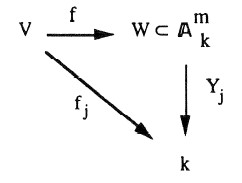
\includegraphics[width=5cm]{68.jpg}\\
		 % \caption{初}
		\end{figure}


		$"\Longrightarrow"$
		如果$ f $是由$F_{1}\cdots,F_{m}$定义的, 那么复合映射就是$P\mapsto F_{j}(P)$, 是一个多项式函数.

		$"\Longleftarrow"$
		如果$\forall  j, f_{j}\in k[V] $, 那么可以在满足$f_{j}=F_{j} mod\ I(V), F_{j}\in k[X_{1},X_{2}\cdots,X_{n}]$的$F_{j}$中选一个,就得到了$ f $的一种由多项式映射给出的定义$(F_{1},F_{2}\cdots,F_{m})$.

		由这个断言可知, 映射$ f $可写成$f=(f_{1},f_{2}\cdots,f_{m})$.

		多项式映射的复合是由简单的方式定义: 如果$V\subset \mathbb{A}^{n}, W\subset \mathbb{A}^{m}, U\subset \mathbb{A}^{l}$是代数集, 且$ f:V\rightarrow W, g:W \rightarrow U  $是多项式映射,那么$g\circ f :V \rightarrow U$仍然的一个多项式映射; 如果$ f $是由$F_{1}\cdots,F_{m}\in k[X_{1},X_{2}\cdots,X_{n}]$定义的且$ g $是由$G_{1}\cdots,G_{l}\in k[Y_{1},Y_{2}\cdots,Y_{m}]$定义, 那么$g\circ f$由$G_{1}(F_{1}\cdots,F_{m})\cdots,G_{l}(F_{1}\cdots,F_{m})\in k[X_{1},X_{2}\cdots,X_{n}]$定义的.

		\textbf{定义} \ 称代数集之间的多项式映射$ f:V \rightarrow W $是同构,如果存在多项式映射 $ g:W \rightarrow V $使$g\circ f=id_{V}, f\circ g=id_{W}$

		几个多项式映射的例子:(2.1)中的参数化$\mathbb{R}^{1}\rightarrow C\subset \mathbb{R}^{2}, t\mapsto (t^{2},t^{3})$或者$(t^{2}-1,t^{3}-t)$, (3.11,b)中讨论的映射$k\rightarrow C\subset \mathbb{A}^{3}_{k}, t\mapsto (t^{3},t^{4},t^{5})$都是多项式映射.并且,在讨论诺特正规化定理时,考虑一个代数集$V\subset \mathbb{A}^{n}_{k}$和由$ m $个$Y_{1},Y_{2}\cdots,Y_{m}$的线性型定义的映射$p:V\rightarrow \mathbb{A}^{m}_{k}$, 因为$Y_{i}$是$X_{i}$的线性型,所以这是多项式映射.

	\section{多项式映射和$ k[V] $}
		\textbf{定理} \ 取$V\subset \mathbb{A}^{n},W\subset \mathbb{A}^{m}$是代数集.

		(I)一个多项式映射$ f:V \rightarrow W $导出一个环同态$f^{*}:k[W]\rightarrow k[V]$, 是由函数的复合定义的, 即如果$g\in k[W]$是多项式函数, 那么$f^{*}(g)=g\circ f$, 并且$g\mapsto g\circ f$定义了一个环同态, 事实上是一个$ k $—代数同态$f^{*}:k[W]\rightarrow k[V]$.

		(II)反过来, 任意一个$ k $—代数同态$\Phi:k[W]\rightarrow k[V]$都是由一个多项式映射$ f:V \rightarrow W $唯一定义的,即$\Phi=f^{*}$.

		因此(I)和(II)表明
		\center  $\{$多项式映射$f:V \rightarrow W \}\longrightarrow $$\{$k-代数同态$\Phi:k[W]\rightarrow k[V]\}$



			  $ f \longmapsto f^{*}$

		\justifying


		是双射.

		(III)如果$ f:V \rightarrow W $和$ g:W \rightarrow U $是多项式映射, 那么两个环同态可复合$(g\circ f)^{*}=f^{*}\circ g^{*}:k[U]\rightarrow k[V]$

		\textbf{证明} \ (I)通过(4.3), $f^{*}(g)$是多项式映射$V\rightarrow k$, 因此$f^{*}(g)\in k[V]$.显然 $f^{*}(a)=a, \forall a\in k$(这里把$ k $看做$ V,W $上的常值函数).最后 $f^{*}$是环同态是形式上的, 因为$ k[W] $和$ k[V] $是函数环.(环结构是由点态定义的, 例如,$g_{1},g_{2}\in k[W]$, 它们的和 $g_{1}+g_{2}$也是作为函数在$ W $上定义的并使得$(g_{1}+g_{2})(P)=g_{1}(P)+g_{2}(P) ,\forall P\in W$; 所以$f^{*}(g_{1}+g_{2})(Q)=(g_{1}+g_{2})(f(Q))= g_{1}(f(Q))+g_{2}(f(Q))= f^{*}g_{1}(Q)+f^{*}g_{2}(Q))$

		(III)可由映射的复合推导出

		(II)的证明需要更多的技巧, 对于$i=1,2\cdots,m$, 令$y_{i}\in k[W]$是$ W $上的第$ i $个坐标函数,所以
		\begin{equation*}
		k[W]=k[y_{1}  \cdots, y_{m}]=k[Y_{1},Y_{2} \cdots,Y_{m}]/I(W)
		\end{equation*}
		现在$\Phi:k[W]\rightarrow k[V]$已经给出, 所以可以用$f_{i}=\Phi(y_{i})$定义$f_{i}\in k[V]$

		考虑映射$f:V \rightarrow \mathbb{A}^{m}_{k}, f(P)=f_{1}(P)\cdots f_{m}(P)$, 由于$f_{i}\in k[V]$, 所以$ f $是多项式映射, 进一步可以断言$ f $把$ V $嵌入到$ W $中,即$f(V)\subset W$.事实上, 假设$G\in I(W)\subset k[Y_{1},Y_{2}\cdots,Y_{m}]$; 那么
		\begin{equation*}
		G(y_{1}\cdots ,y_{m})=0\in k[W]
		\end{equation*}
		左边是我把环元素$y_{i}$代入多项式表达式$ G $, 所以$\Phi(G(y_{1}\cdots y_{m}))=0\in k[V]$; 但$ \Phi$是$ k $-代数同态, 所以
		\begin{equation*}
		k[V]\ni 0=\Phi(G(y_{1}\cdots, y_{m}))=G(\Phi(y_{1})\cdots ,\Phi(y_{m}))=G(f_{1}\cdots ,f_{m})
		\end{equation*}
		$f{i}$是$ V $上的函数, $G(f_{1}\cdots f_{m})\in k[V]$是由函数$P\mapsto G(f_{1}(P))\cdots ,f_{m}(P))$定义的. 这证明了对$P\in V$和每一个$G\in I(W),f(P)$的坐标($f_{1}(P))\cdots ,f_{m}(P)$)满足$G(f_{1}(P))\cdots ,f_{m}(P))=0$.因为$ W $是由$G\in I(W)$的零点定义的$\mathbb{A}^{m}_{k}$的子集,它满足$f(P)\in W$. 这证明了上面给出的$ f $是多项式映射$ f:V \rightarrow W $.为了检验两个$ k $-代数同态$f^{*},\Phi:k[W]\rightarrow k[V]$相符, 只要证明它们的生成元相同,即$f^{*}(y_{i})=\Phi(y_{i})$,从$ f $的构造中可以发现这个事实.一个相似的论证可以表明映射$ f $是由$f^{*}(y_{i})=\Phi(y_{i})$  唯一决定的.
	\section{推论}一个多项式映射$ f:V \rightarrow W $是同构当且仅当$f^{*}:k[W]\rightarrow k[V]$是同构.

		\textbf{例子} \ $  k $是无限域,多项式映射
		\begin{equation*}
		\varphi:\mathbb{A}^{1}_{k}\rightarrow C:(Y^{2}=X^{3}) \subset \mathbb{A}^{2}_{k},  T\mapsto (T^{2},T^{3})
		\end{equation*}
		不是同构.因为这种情况下, 同态
		\begin{equation*}
		\varphi^{*}:k[C]=k[X,Y]/(Y^{2}-X^{3})\rightarrow k[T]
		\end{equation*}
		是由$X\mapsto T^{2},Y\mapsto T^{3}$给出的.$\varphi^{*}$的象是由$T^{2},T^{3}$生成的$ k $-代数,即$k[T^{2},T^{3}]\subsetneq k[T]$.
		
		注意到$\varphi$是双射,所以有一个逆映射$\psi :C\rightarrow \mathbb{A}^{1}_{k}$,如果$ X=Y=0 $,则$(X,Y)\mapsto 0$, 否则$(X,Y)\mapsto Y/X$.所以$\varphi$为什么不是同构呢?重点是$ C $上的多项式比$\mathbb{A}^{1}_{k}$上的少.
	\section{仿射簇}
		$ k $是一个域, 仿射簇是同构意义下的不可约代数集$V\subset $ A $^{n}_{k}$.

		定理4.4告诉我们坐标环$ k[V] $是$ V $的同构类中的不变量.这样我就可以少用$V\subset \mathbb{A}^{n}_{k}$周围的空间定义簇;后面提出的仿射簇总是上述意义下的.

		\textbf{定义} \ $ k $上的仿射簇是集合$ V $和关于$ k $-值函数$f:V\rightarrow k$的环$ k[V] $,使得

		(i)$ k[V] $是有限生成的$ k $-代数,

		(ii)从$ k[V] $选择一些生成元$x_{1}  \cdots, x_{n}$,映射
		\center $ V \rightarrow  \mathbb{A}^{n}_{k}$


		$P\mapsto x_{1}(P)  \cdots, x_{n}(P)$

		\justifying
		把$ V $作为不可约代数集嵌入到 $ \mathbb{A} ^{n}_{k}$.
		
		
		\section{函数域}$ V $是仿射簇, 那么$ V $的坐标环$ k[V] $是整环,其中的元素是$ V $上的$ k $值函数.

		\textbf{定义} \ $ V $的函数域$ k(V) $是关于在$ k[V] $上的分式$ k(V)=Quot(k[V]) $的域.一个元素$f\in k(V)$是$ V $上的有理函数;需要注意$f\in k(V)$是由商$ f=g/h $定义的,其中$g,h\in k[V]$且$h\neq 0$.	

		先验$ f $不是$ V $上的函数,因为在$ h $的零点处$ f $无定义, 可是$ f $在$P\in V,h(P)\neq 0$处有定义,所以$ f $至少是一个“部分定义函数”,下面介绍一些术语支持这个想法.

		\textbf{定义} 取$f\in k(V),P\in V$, 称$ f $是在$ P $上正则的或者$ P $在$ f $的定义域内, 如果存在一种表达$ f=g/h $, 其中$g,h\in k[V]$且$h(P)\neq 0$.

		值得注意的是$ k[V] $通常不是唯一分解整环,所以$f\in k(V)$可能有本质不同的表示法$ f=g/h $, 见\textit{习题4.9}中的例子.

		称

		\begin{equation*}dom \ f=\{P\in V\vert f\text{在$ P $上正则}\}\end{equation*}
		
		为$ f $的定义域,且

		\begin{equation*}O_{V, P}=\{f \in k (V) | f \text{在$ P $上正则}\}=k[V]\left[\left\{h^{-1} | h(P) \neq 0\right\}\right]\end{equation*}

		\justifying
		那么$O_{V, P}\subset k(V)$是子环,是$ V $在$ P $点的局部环.
	\section{定理}
		(I)$ dom\ f $在Zariski拓扑下是稠密的开集.

		假设$ k $是代数闭域;那么

		(II)$dom \ f=V\iff f\in k[V]$(即多项式函数=正则有理函数),

		进一步,对任意的$h\in k[V]$,令
		\begin{equation*}
		V_{h}=V\backslash V(h)=\{P\in V \vert h(P)\neq 0\}
		\end{equation*}
		那么
		
		(III)$V_{h}\subset dom \ f \iff f\in k[V][h^{-1}]$.

		\textbf{证明} \ 定义$f\in k(V)$的分母的理想

		\center $ D_{f}=\{ h\in k[V] \vert hf\in k[V] \}\subset k[V]$
		
			  $ =\{ h\in k[V] \vert$ 存在一个表示$ f=g/h $, 其中$g\in k[V]\}\cup \{0\}$

		\justifying

		从第一行可以看出, $D_{f}$是$ k[V] $的理想.证明:
		\begin{equation*}
		V\backslash dom \ f=\{P\in V \vert h(P)= 0 ,\forall h\in D_{f}\}=V(D_{f})
		\end{equation*}
		所以$V\backslash dom \ f$是$ V $的代数集,因此$dom \ f=V\backslash V(D_{f})$是闭集的补集,所以是Zariski拓扑下的开集. $ dom \ f $显然是非空的,所以由推定理4.2知是稠密的.

		使用零点定理的(b),
		\begin{equation*}
		dom f=V\iff V(D_{f})=\varnothing \iff 1\in D_{f} \iff f\in k[V]
		\end{equation*}
		最后,

	\begin{equation*}
		V_{h}\subset dom \ f \iff h \text{在}V(D_{f})\text{上为}0,
		\end{equation*}

		使用零点定理的(c),
		
		\begin{equation*}\iff h^{n}\in D_{f},\text{对某些} n ,\text{即}f=g/h^{n}\in k[V][h^{-1}]\end{equation*}

	\section{有理映射}取$ V $是仿射簇

		\textbf{定义} \ 一个有理映射$f:V\dashrightarrow \mathbb{A}^{n}_{k}$是由有理函数$f_{1}\cdots ,f_{n}$部分定义的映射,即

		\begin{equation*}
		f(P)=(f_{1}(P)\cdots, f_{n}(P)) ,\forall P\in \bigcap dom \ f_{i}
		\end{equation*}

		根据定义,$dom \ f=\bigcap dom \ f_{i}$, 称$f $在$ P\in V $点是正则的当且仅当$P\in dom f$. 两个仿射簇$V\subset \mathbb{A}^{n},W\subset \mathbb{A}^{m}$之间的有理映射$V\dashrightarrow W$被定义成有理映射$f:V\dashrightarrow \mathbb{A}^{m}$,使得$f(dom \ f)\subset W.$

		在(4.3)的结尾有两个有理映射的例子.

	\section{有理映射的复合映射}
		有理映射$ f:V \dashrightarrow W $和$ g:W \dashrightarrow U $的复合映射$(g\circ f)$可能没有定义.这个困难是由有理映射不是映射造成的,显然复合映射定义在$dom \ f\cap f^{-1}(dom \ g)$; 可是这很可能是空集(见\textit{练习4.10}).

		在代数表示上,相同的问题也会发生:假如$ f $是由$f_{1}\cdots ,f_{m}\in k(V)$给出, 那么
		\begin{equation*}
		f:V \dashrightarrow W\subset \mathbb{A}^{m}
		\end{equation*}
		\begin{equation*}
		P \mapsto f_{1}(P)\cdots, f_{m}(P)
		\end{equation*}
		对$P\in \bigcap dom \ f_{i}$;任意的$g\in k[W]$对一些$G\in k[Y_{1}\cdots,Y_{m}]$是 $g=G \ mod \ I(W)$ 的形式, 且$g\circ f=G(f_{1}\cdots ,f_{m})$ 在$ k(V) $上是良定义的. 所以像(4.4)一样,有一个$ k $-代数同态
		\begin{equation*}
		f^{*}:k[W]\rightarrow k(V)
		\end{equation*}
		对应$ f $.可是,如果$h\in k[W]$是$f^{*}$的核, $f^{*}(g/h)$可能没意义,所以$f^{*}$不能延拓到域同态$k(W)\rightarrow k(V)$.

		\textbf{定义} \ 称$f:V \dashrightarrow W$是显性的如果$ f(dom \ f) $在$ W $中在Zariski拓扑下是稠密的.

		几何上,这意味着对任意的有理映射$g:W\dashrightarrow U,  f^{-1}(dom \ g)\subset dom \ f$是稠密的开集,所以$g\circ f$定义在V上的稠密的开集上,所以是部分定义的映射$V\dashrightarrow U$.

		代数上,

		\center  $ f $是显性的 $\iff f^{*}:k[W]\rightarrow k(V)$是单射

		\justifying
		对给定的$g\in k[W]$,
		\begin{equation*}
		g\in ker f^{*} \iff f(dom f)\subset V(g)
		\end{equation*}

		即$f^{*}$不是单射当且仅当$ f(dom \ f) $是$ W $的真子集.

		显然,有理映射$ f $和$ g $的复合映射$g\circ f$中$ f$是 显性的:$g\circ f$是有理映射,由$f^{*}(g_{i})$组成.注意到$g\circ f$的定义域包含 $f^{-1}(dom \ g)\cap dom f$, 但可能会更大(见\textit{习题4.6})
	\section{定理}
		(I)一个显性的的有理映射$f:V\dashrightarrow W$定义一个域同态$f^{*}:k(W)\rightarrow k(V)$.

		(II)反过来,一个$ k $-同态$\Phi: k(W)\rightarrow k(V)$来自一个唯一定义的有理映射$f:V\dashrightarrow W$.

		(III)如果$ f $和$ g $是显性的的,则$(g\circ f)^{*}=f^{*}\circ g^{*}$

		证明仅仅需要对(4.4)做微小的变动.

	\section{来自仿射簇开集的态射}
		取$ V,W $是仿射簇,$U\subset V$是开集.

		\textbf{定义} \ 态射$f:V\rightarrow W$是有理映射$f:V\dashrightarrow W$使得$U\subset dom f$,所以f在每一点$P\in U$是正则的.

		如果$U_{1}\subset V,U_{2}\subset W$是开集,那么一个态射$f:U_{1}\rightarrow U_{2}$就是一个态射$f:U_{1}\rightarrow W$,满足$f(U_{1})\subset U_{2}$. 同构是指一个态射两边都有逆态射.

		如果$ V,W $是仿射簇,那么由同构定理(4.8,II)
		\center  $\{$态射$f:V\rightarrow W\}=\{$多项式映射$f:V\rightarrow W\}$


		\justifying
		\textbf{例子} \ (2.1)中的三次曲线参数化$\mathbb{A}^{1} \rightarrow C:(Y^{2}=X^{3}) $导出同态$\mathbb{A}^{1}\backslash \{0\}\backsimeq C\backslash \{0,0\}$,细节见\textit{习题4.5}.


	\section{标准的开集}
		取$ V $是一个仿射簇.对于$ f \in k[V] $,记$ V_{f} $为开集$ V_{f} = V \backslash V(f) = \{P\in|f(P) \neq 0 \} $.则$ V_{f} $被称作$ V $上的标准开集

		\textbf{定理} \ $V_{f}$是到仿射簇的同构,且$k[V_{f}]=k[V][f^{-1}].$

		\textbf{证明}\ 想法是考虑函数$f^{-1}$的图像;使用(3.10)中零点定理$(b)\Rightarrow(c)$证明中相似的方法.
		\begin{figure}[h]
		  \centering
		  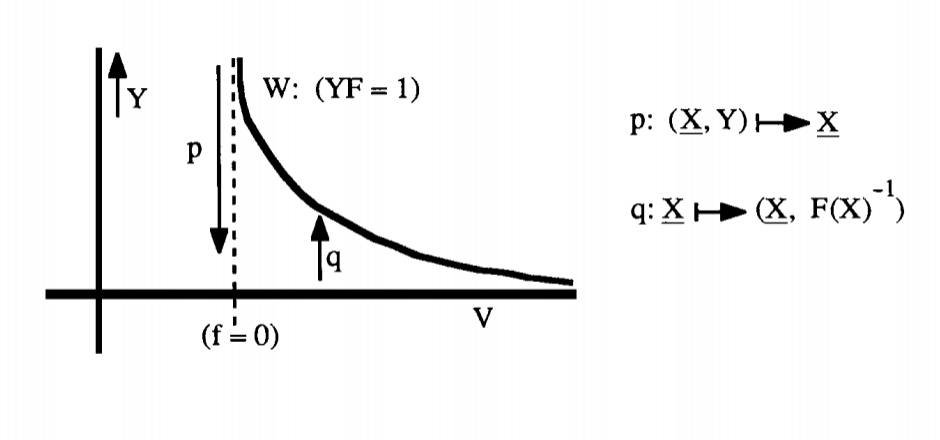
\includegraphics[width=10cm]{75.jpg}\\
		 % \caption{初}
		\end{figure}

		取$J=I(V)\subset k[X_{1},X_{2}\cdots,X_{n}]$,选择$F\in k[X_{1},X_{2}\cdots,X_{n}]$使$f=F \ mod \ I(V)$.现在定义$I=(J,YF-1)\subset k[X_{1},X_{2}\cdots,X_{n},Y]$,令$V(I)=W\subset \mathbb{A}^{n+1}.$
		很容易检验图中的映射是$V_{f}$和W之间的可逆态射,关于坐标环的说明在(4.8,III).

		标准开集$V_{f}$是很重要的, 因为它形成了$ V $的Zariski拓扑的一组基:每一个开集$U\subset V$都是一些$V_{f}$的并集(因为每一个闭集的形式都是$V(I)=\bigcap_{f \in I} V(f)$).因此结果就证明了每一个开集$U\subset V$都是仿射簇开集$V_{f}$的并集.



\chapter{射影几何和双有理几何}
	本章节的第一部分旨在概括第三章和第四章关于射影簇的内容.剩下的部分主要关于双有理几何,其中用到了第四章最后部分的函数域$ k(V) $,这一部分在射影或者仿射情景下也是适合的.
	
	\setcounter{section}{-1}
	\section{为什么讨论射影簇}
		三次曲线
		\begin{equation*}
		C :\left( Y ^{2} Z = X ^{3}+ aXZ ^{2}+ bZ ^{3}\right) \subset \mathbb{P} ^{2}
		\end{equation*}
		是两个仿射曲线的并:
		\begin{equation*}
		\left. C _{0}:\left( y ^{2}= x ^{3}+ ax + b \right) \subset \mathbb{A} ^{2} \quad  (C \text{中取} (Z = 1) \text{截面}\right)
		\end{equation*}
		和
		\begin{equation*}
		\left. C _{1}:\left( z _{1}= x _{1}^{3}+ axz _{1}^{2}+ bz _{1}^{3}\right) \subset \mathbb{A} ^{2}   (C \text{中取} (Y = 1) \text{截面}\right)
		\end{equation*}
		这种并是由同构
		\begin{equation*}
		C _{0} \backslash( y =0) \longrightarrow  C _{1} \backslash\left( z _{1}=0\right)
		\end{equation*}
		\begin{equation*}
		( x , y ) \mapsto( x / y , 1 / y )
		\end{equation*}
		所胶合的.
		
		
		作为一个较为简单的例子, 有着齐次坐标 $( X , Y )$的$\mathbb{P}^{1}$是两个分别具有坐标$ x_{0},y_{1} $的 $\mathbb{A}^{1}$的并,这种并由同构
		\begin{equation*}
		\mathbb{A}^{1} \backslash\left(x_{0}=0\right)\rightarrow \mathbb{A}^{1} \backslash\left(y_{1}=0\right)
		\end{equation*}
		\begin{equation*}
		x _{0} \quad \mapsto \quad 1 / x _{0}
		\end{equation*}
		所胶合的.
		
		
		\begin{figure}[h]
			\centering
			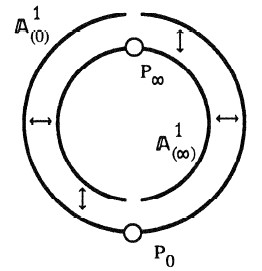
\includegraphics[width=5cm]{50.jpg}\\
			\caption*{一个简单的图例,其中'$ \leftrightarrow $'代表同构}
		\end{figure}
	
		
		重点是,射影簇是严格大于仿射簇的. 事实上,根据之后会提到的自然态射的概念, 可以看出不存在非恒定态射$\mathbb{P} ^{1} \rightarrow \mathbb{A} ^{n}$或$C \rightarrow \mathbb{A}^{n}$ 对于任意的$n$ (可见\textit{习题5.1}和\textit{习题5.12}).
		
		
		解决该问题的一种方法是采用适当的模来胶合,而将“抽象簇” $ V $的概念定义为仿射簇的并集$ V = \bigcup V _ {i} $.类似于拓扑中流形的定义,这是一个有吸引力的想法,但是它带来了更多的技术难题.使用射影簇可以通过在现成的环绕空间$ \mathbb{P} ^ {n}$中工作来避免这些问题,因此(除了对齐次多项式有所了解之外),它们比仿射簇更难研究.实际上,尽管在初级阶段可能还不清楚,但是射影簇在相当可观的范围内为研究簇提供了自然的框架.
		
	\section{分次环和齐次理想}
		\textbf{定义}\ 一个多项式$f \in k \left[ X _{0} \ldots X _{ n }\right]$是$ d $次齐次的,如果
		\begin{equation*}
			f =\sum a _{ i _{0}} \cdots _{i_{ n }} X _{0}^{ i _{0}} \cdots X _{ n }^{ i _{ n }} \text{其中} a _{ i _{0}} \ldots _{i_{ n }} \neq 0 \text{当且仅当} i _{0}+\ldots i _{ n }= d
		\end{equation*}
		对于任意$f \in k \left[ X _{0} \ldots X _{ n }\right]$存在一个唯一的表达$f = f _{0}+ f _{1}+\ldots f _{ N }$ 其中$f _{ d }$ 是具有$ d $次齐次的多项式,而$d =0,1, \ldots N$.
		
		
		\textbf{命题}\ 如果$f$ 是$ d $次齐次的,则
		\begin{equation*}
		f \left(\lambda X _{0}, \ldots \lambda X _{ n }\right)=\lambda^{d} f \left( X _{0}, \ldots X _{ n }\right) \quad \text {对于任意}\lambda \in k\text{都成立}
		\end{equation*}
		如果$k$是一个无限域,则反之亦成立.
		
		
		\textbf{证明}\  $"\Rightarrow" $ \ $ f $是$ d $次齐次多项式,
		
		$f \left(\lambda X _{0}, \ldots \lambda X _{ n }\right)$
		
		
		$=\sum a _{ i _{0}\cdots i _{ n } }(\lambda X _{0})^{ i _{0}} \ldots (\lambda X _{ n })^{ i _{ n }}$
		
		
		$=\sum a _{ i _{0}\cdots i _{ n } }(\lambda)^{i _{0}+ \ldots i _{ n }}X _{0}^{ i _{0}} \ldots X _{ n }^{ i _{ n }}$
		
		
		$=\lambda^{d}\sum a _{ i _{0}\cdots i _{ n } }X _{0}^{ i _{0}} \ldots X _{ n }^{ i _{ n }}$
		
		
		$=\lambda^{d}f \left( X _{0}, \ldots X _{ n }\right)$
		
		$"\Leftarrow" $, \ 设$f=f_{m}+f_{n}	$, 如果$m\neq n	,\lambda \neq 0,1$,则
		
		$f \left(\lambda X _{0}, \ldots \lambda X _{ n }\right)$
		
		$=f_{m} \left(\lambda X _{0}, \ldots \lambda X _{ n }\right)+f_{n} \left(\lambda X _{0}, \ldots \lambda X _{ n }\right)$
		
		$=\lambda^{m}f_{m}+\lambda^{n}f_{n}$
		
		因为$ k $为无限域,所以$\lambda^{m} \neq \lambda^{n},(\lambda \neq 0,1,-1)$,所以上式$ \neq \lambda^{d}(f_{m}+f_{n}),\forall d\in k$
		
		即$f \left(\lambda X _{0}, \ldots \lambda X _{ n }\right) \neq \lambda^{d}f \left( X _{0}, \ldots X _{ n }\right),\forall d\in k$ ,矛盾.
		
		
		\textbf{定义}\ 一个理想$I \subset k \left[ X _{0}, \ldots X _{ n }\right]$是齐次的,如果对于所有$f \in I$,在$ f $的齐次分解$f = f _{0}+ f _{1}+\ldots f _{ N }$中,对于$ \forall i $有$f _{ i } \in I$.
		
		
		这等价于$ I $是由(有限个)齐次多项式生成的.
		
		
	\section{齐次的$ V-I $对应}
		取$\mathbb{P} ^{n}_{k}$ 是一个在域$ k $上的$ n- $维射影空间,其中有齐次坐标$X _{0} . . X _{ n }$.则$f \in k \left[ X _{0}, \ldots X _{ n }\right]$不是一个在$\mathbb{P} ^{ n }_{k} $上的函数:由定义,$\mathbb{P} ^{ n }_{ k }= k ^{ n +1} \backslash\{0\} / \sim$,其中$\sim$是一个等价关系,这个等价关系是$\left( X _{0}, \ldots X _{ n }\right) \sim\left(\lambda X _{0}, \ldots \lambda X _{ n }\right)$其中$\lambda \in k \backslash\{0\} $;而$ f $是一个在$k ^{n+1}$上的函数.但是,对于$P \in \mathbb{P}^{n} ,$如果$ f $是齐次的,那么条件$f ( P )=0$就是良定义的:假设$P =\left( X _{0}: \dots X _{ n }\right)$,则$\left(X_{0}, \ldots X_{n}\right)$是$ P $在 $k^{n+1} \backslash\{0\}$上的等价类的代表元.因为$f(\lambda \underline{X})=\lambda^{d} f(\underline{X}),$如果$f\left(X_{0}, \ldots X_{n}\right)=0$ 那么就有$f\left(\lambda X_{0}, \ldots \lambda X_{n}\right)=0,$因此条件$f ( P )=0$是独立于代表元的选取的.出于这种想法像以前一样定义对应$ V,I $
		\begin{equation*}
		\left\{\text {齐次理想 } J \subset k \left[ X _{0}, \dots X _{ n }\right]\right\} \quad \stackrel{ V , I }{\longleftrightarrow}\left\{\text { 子集} X \in \mathbb{P} _{ k }\right\}
		\end{equation*}
		其中
		\begin{equation*}
		V ( J )=\left\{ P \in \mathbb{P} ^{ n }_{k} | f ( P )=0, \forall \text { 齐次} f \in J \right\}
		\end{equation*}
		\begin{equation*}
		I ( X )=\left\{ f \in k \left[ X _{0}, \ldots X _{ n }\right] |  \text { 对于所有 } P \in X \text{有} f ( P )=0\right\}
		\end{equation*}
		作为一个练习,想一想为什么 $I ( X )$ 是一个齐次理想.
		
		对应$ V $和$ I $满足仿射条件下的$ V,I $的一样形式的属性(例如$V \left( J _{1}+ J _{2}\right)=  V \left( J _{1}\right) \cap V \left( J _{2}\right) $依然成立). $V ( I )$的子集是$\mathbb{P}^{n} _{ k }$的代数子集,类似在仿射条件下的结论,如果在 $\mathbb{P} ^{n}_{k}$上定义代数子集是闭集就能构造一个Zariski拓扑.
		
		
	\section{射影条件下的零点定理}
		在仿射意义的对应下,对于任意理想$ J $的$I ( V ( J )) \supset rad J$和对于任意代数集$ X $的$ V(I(X))  = X$是完全形式化的.只有一点需要注意:平凡的理想$(1) = k \left[ X _{0} \ldots X _{ n }\right]$(即整个环)在对应下定义了$k ^{ n +1}$的空集,因此在$\mathbb{P} ^{n}_{ k }$中同样有类似的结论;但是,理想$\left(X_{0} \ldots X_{n}\right)$在 $k ^{n+1}$上同样对应到 $\{0\}$,即在$\mathbb{P} ^{n}_{ k }$上同样对应空集.理想$\left(X_{0} \ldots X_{n}\right)$是定理中几个论述的例外,传统上被称为'无关理想'.
		
		
		\textbf{定理}\ 假设$ k $是一个代数闭域,则
		\begin{enumerate}[(i)]
			\item $ V ( J )=\varnothing  \Longleftrightarrow rad J \supset\left( X _{0}, \ldots X _{ n }\right)$
			\item 若$V ( J ) \neq \varnothing$则$ I ( V ( J ))= rad J $
		\end{enumerate}
		
		
		\textbf{推论}\ $ I $和$ V $确定可逆的双射
		\begin{equation*}
		\left\{\begin{array}{l}
		{\text {齐次根理想} J \subset k [x_{0}, \cdots x_{n} ]} \\
		{\text { 其中} J \neq k [x_{0}, \ldots x_{n} ]} 
		\end{array}\right\}
		 \longleftrightarrow
		 \left\{\begin{array}{c}
		{\text { 代数子集 }} \\
		{X \subset \mathbb{P} ^{n}}
		\end{array}\right\}
		\end{equation*}
		
		$\qquad \quad \qquad\qquad \qquad \qquad \qquad \cup \qquad \qquad \qquad\qquad \qquad \qquad \qquad \cup $
		\begin{equation*}
		\qquad\quad
		\left\{\begin{array}{l}
		{\text {齐次素理想} J \subset k [x_{0}, \cdots x_{n} ]} \\
		{\text { 其中} J \neq k [x_{0}, \ldots x_{n} ]} 
		\end{array}\right\}
		\longleftrightarrow
		\left\{\begin{array}{c}
		{\text { 不可约代数子集 }} \\
		{X \subset \mathbb{P} ^{n}}
		\end{array}\right\}
		\end{equation*}
		
		
		\textbf{证明}\ 取$\pi: \mathbb{A} ^{n+1} \backslash\{0\} \rightarrow \mathbb{P}^{n}$是一个定义了$\mathbb{P} ^{n}$的映射.对于齐次理想 $J \subset k \left[ X _{0}, X _{ n }\right]$,记$V ^{ a }( J ) \subset \mathbb{A} ^{ n +1}$是由$ J $定义的仿射代数集.此时因为$ J $是齐次的,所以对$V ^{ a }( J )$有:
		\begin{equation*}
		\left(\alpha_{0}, \dots \alpha_{n}\right) \in V ^{ a }( J ) \Longleftrightarrow\left(\lambda \alpha_{0}, \dots \alpha_{n}\right) \in V ^{ a ( J )}
		\end{equation*}
		并且$V ( J )= V ^{ a ( J )} \backslash\{0\} / \sim \subset \mathbb{P} ^{ n } .$因此有
		\begin{equation*}
		V ( J )=\varnothing \Longleftrightarrow V ^{ a }( J ) \subset\{0\} \Longleftrightarrow \operatorname{rad} J \supset\left( X _{0} \ldots X _{ n }\right)
		\end{equation*}
		其中最后一部分用到了仿射条件下的零点定理.并且,如果$V ( J ) \neq \varnothing$则
		\begin{equation*}
		f \in I ( V ( J )) \Longleftrightarrow f \in I \left( V ^{ a }( J )\right) \Longleftrightarrow f \in rad J 
		\end{equation*}
		则证毕.
		
		
		上面提到过的仿射子集$V ^{ a }( J )$ 被称作在射影代数子集$ V(J) $上的仿射锥.
		
		
	\section{$ V $上的有理函数}
		取 $V \subset \mathbb{P} ^{ n }_{k}$是一个不可约代数集, 而$I ( V ) \subset k \left[ X _{0}, \ldots X _{ n }\right]$ 是它的理想; 则此时不能用直接的方法来通过多项式定义$ V $上的正则函数: 元素 $F \in k \left[ X _{0}, \ldots X _{ n }\right]$给出了在$ V $上仿射锥上的一个函数,但是除非$ F $是0次齐次的,否则这个函数在所有等价类上都是一个常数,即这个函数总是一个常数.
		
		
		作为一个起点,可以先从有理函数开始:
		
		
		\textbf{定义}\ 在$V$上的有理函数$f : V \dashrightarrow k$是一个由$f ( P )= g ( P ) / h ( P )$定义的(部分定义)函数,其中$ g , h \in k \left[ X _{0}, \ldots X _{ n }\right]$是具有相同次数的齐次多项式.
		
		注意,此时有$h ( P ) \neq 0,$ 则商$g ( P ) / h ( P )$是良定义的, 因此
		\begin{equation*}
		g (\lambda \underline{ X }) / h (\lambda \underline{ X })=\lambda^{ d}  g (\underline{ X }) / \lambda^{d} h (\underline{ X })= g (\underline{ X }) / h (\underline{ X }) \quad \text {其中} 0 \neq \lambda \in k
		\end{equation*}
		
		
		显然,当且仅当$h ^{\prime} g - g ^{\prime} h \in I ( V )$时,$g / h$和$g ^{\prime} / h ^{\prime}$定义同一个有理函数,因此所有有理函数组成的集是一个域
		\begin{equation*}
		k ( V )=\left\{ g / h | \text {齐次且次数相同的} g , h \in k \left[ X _{0}, \ldots X _{ n }\right], h \notin I ( V )\right\} / \sim
		\end{equation*}
		其中$\sim$ 是等价关系
		\begin{equation*}
		g / h \sim g ^{\prime} / h ^{\prime} \Longleftrightarrow h ^{\prime} g - g ^{\prime} h \in I ( V )
		\end{equation*}
		$k ( V )$ 是 $V$上的有理函数域. 
		
		
		接下来的定义就像仿射情形的情况. 对于$f \in k ( V )$ 和 $P \in V ,$ 称$f$在$P$上是正则的,如果存在表达式$f = g / h ,$ 其中$g , h$是相同次数的齐次多项式,并且使得 $h ( P ) \neq 0 .$ 记
		\begin{equation*}
		dom f =\{ P \in V | f \text {在} P \text{上是正则的}\}
		\end{equation*}
		和
		\begin{equation*}
		O _{ V , P }=\{ f \in k ( V ) | f \text {在} P \text{上是正则的}\}
		\end{equation*}
		显然, $dom f \subset V$在 $V$上是一个Zariski稠密开集 (证明同$(4.8, I )$) 并且$O _{ V , P } \subset k ( V )$ 是一个子环.
		
	\section{射影簇的仿射覆盖}
	
		取$V \subset \mathbb{P}^{n}$ 是一个不可约代数集,为简单起见,假设对任意$ i $存在$V\not\subset \left(X_{i}=0\right)$.已知,$\mathbb{P}^{n}$可以由$( n +1)$ 个仿射片$\mathbb{A} ^{ n }_{( i )}$覆盖,其中有仿射(非齐次)坐标$X _{0}^{( i )}, \ldots X _{ i -1}^{( i )}, X _{ i +1}^{( i )}, \ldots X _{ n }^{( i )},$ 其中
		\begin{equation*}
		X _{ j }^{( i )}= X _{ j } / X _{ i } \quad \text {其中} j \neq i
		\end{equation*}
		记$V_{(i)}=V \cap \mathbb{A}^{n}_{(i)} .$则 $V_{(i)} \subset \mathbb{A}^{n}_{(i)}$ 显然是一个仿射代数集,因为
		\begin{equation*}
		\begin{aligned}
		V _{(0)} & \ni P =\left(1, x _{1}^{(0)}, \ldots x_{ n} ^{(0)}\right) \\
		& \Longleftrightarrow f \left(1, x _{1}^{(0)}, \ldots x _{ n }^{(0)}\right)=0  \text {对于所有齐次} f \in I ( V )
		\end{aligned}
		\end{equation*}
		这是在$ P $的坐标 $\left(x_{1}^{(0)}, \ldots x_{n}^{(0)}\right)$ 上的一组多项式关系. 为了说清楚这些事,不妨取$i =0$,而结论在其他的仿射片$V _{( i )} $中依然成立. 其中$V _{( i )}$被称为$V$的基准仿射片.
		
		
		\textbf{命题}. (i) 对应 $V  \rightarrow V _{(0)}= V \cap \mathbb{A} ^{ n }_{(0)}$给出了一个双射
		\begin{equation*}
		\left\{
		\text {不可约代数子集} V\subset \mathbb{P}^{n} | V \not\subset(X_{0} = 0)
		\right\}
		\longleftrightarrow
		\left\{
		\text {不可约代数子集} V_{(0)}\subset \mathbb{A}^{n}_{(0)}
		\right\}
		\end{equation*}
		逆对应由Zaraski拓扑的闭包给出.
		
		
		(ii)记$I ^{ h }( V ) \subset k \left[ X _{0}, \ldots X _{ n }\right]$ 是$V \subset \mathbb{P} ^{ n }$的齐次理想且$I ^{ a }\left( V _{(0)}\right) \subset k \left[ X _{1}, \ldots X _{ n }\right]$是$V _{(0)} \subset A ^{ n }_{(0)} $如同第三章那样的一般非齐次理想,则 对$I ^{ h }( V )$和$I ^{ a }\left( V _{(0)}\right)$有:
		\begin{equation*}
		I ^{ a }=\left\{ f \left(1, X _{1}, \ldots X _{ n }\right) | f \in I ^{ h }( V )\right\}
		\end{equation*}
		且
		\begin{equation*}
		\left. I ^{ h }( V )_{ d }=\left\{ X _{0}^{d}  f \left( X _{1} / X _{0}, \dots\right. X _{ n } / X _{0}\right) | f \in I ^{ a} ( V_{(0)}), \text {其中 deg } f \leq d \right\}
		\end{equation*}
		其中$I ^{ h }( V )_{ d }$ 的下标代表这是具有次数$ d $的片. 
		
		
		(iii) $k ( V ) \cong k ( V (0)),$ 并且对于$f \in k ( V ),$$f$的环作为在$V _{(0)}$上的函数是 $V _{(0)} \cap dom f$
		
		
		
		\textbf{证明} (i)和(ii)易证. (iii)如果 $g, h \in k [ X_{0}, . . X_{n}]$ 是$ d $次齐次的, 且$h \notin I ( V ),$ 则$g / h \in k ( V )$在 $V _{(0)}$上的限制是函数
		\begin{equation*}
		g \left(1, X _{1} / X _{0}, \ldots X _{ n } / X _{0}\right) / h \left(1, X _{1} / X _{0} \ldots X _{ n } / X _{0}\right)
		\end{equation*}
		这定义了一个映射$k ( V ) \rightarrow k \left( V _{(0)}\right),$ 而它的逆是显然的.
		
		
	\section{有理映射和态射}
		在射影(或仿射)簇之间的有理映射可以用$ k(V) $来定义:如果$ V \subset \mathbb{P}^{n} $是一个不可约代数集,一个有理映射$V \dashrightarrow \mathbb{A} ^{ m }$是一个由$P \mapsto (f_{1}(P), \dots f_{m}(P))$部分定义的映射,其中$f_{1}, . . f_{m} \in k (V)$. 一个有理映射$V \dashrightarrow \mathbb{P} ^{ m }$是由$P \mapsto\left( f _{0}( P ): f _{1}( P ): \ldots f _{ m }( P )\right)$定义的映射,其中$f _{0}, f _{1}, . . f _{ m } \in k ( V )$.需要注意,如果$g \in k ( V )$是一个非零元, 则$gf _{0}, gf _{1}, gf_{ m }$定义了同样的有理映射. 因此,(假设 $ V$ 并不会映到一个更小的射影空间$( X _{0}=0)$),就有可能假设处处都有$f_{0}=1$.
		
		
		那么,显然在两个集合
		\begin{equation*}
		\left\{\text {有理映射 } f : V \dashrightarrow \mathbb{A} ^{ m } \subset \mathbb{P} ^{ m }\right\}
		\end{equation*}
		和
		\begin{equation*}
		\left\{\text {有理映射} f : V \dashrightarrow \mathbb{P} ^{ m } | f ( V ) \not\subset\left( X _{0}=0\right)\right\}
		\end{equation*}
		间存在一个双射,这是因为任何一种映射都是由$ m $个元素$f _{ i } \in k ( V )$给出的.
		
		
		\textbf{定义}\ 一个有理映射$f : V \dashrightarrow \mathbb{P} ^{ m }$ 在$P \in V$上是正则的,如果存在表达 $f =\left( f _{0}, f _{1}, \ldots f _{ m }\right)$使得
		\begin{enumerate}[(i)]
			\item $f _{0}, \dots f _{ m }$都在$ P $上是正则的
			\item 至少有一个$f_{i}(P) \neq 0$
		\end{enumerate}
	
		在这里,第二个条件的意义是使得$f_{i}$间的比值与$ P $相关.如果$f$ 在$P$上是正则的 (像之前一样,这可以由$P \in dom f$来表达 ),则$f : U \rightarrow \mathbb{A} ^{ m }_{(i)} \subset \mathbb{P} ^{ m }$ 在一个合适的开邻域
		$P \in U \subset V$上是态射: 取$U=\bigcap_{j} dom\left(f_{j} / f_{i}\right)$ 其中 $f_{i}(P) \neq 0 ;$ 则$f$是一个由$\left\{ f _{ j } / f _{ i }\right\}_{ j= 0,1, \ldots m }$定义的态射.
		
		
		如果 $U \subset V$ 是在射影簇 $V$上的一个开子集,则态射
		$f : U \rightarrow W$ 是一个有理映射 $f : V \dashrightarrow W$ 使得 $dom f \supset U$.因此态射实际上就是一个在$ U $上处处正则的有理映射.
		
	\section{一些实例}
		\textbf{(I) 有理正规曲线}
		
		
		 这是同构嵌入的一个简单例子:
		 
		 
		$f: \mathbb{P} ^{1} \stackrel{\cong}{\longrightarrow} C \subset \mathbb{P}^{m}$概括了$(1.7)$中的参数化椭圆, 这种概括在射影和代数的几何中也是成立的. 
	  
	  
	  	定义
		\begin{equation*}
		f : \mathbb{P} ^{1} \rightarrow \mathbb{P} ^{ m } \quad \text {其中 } \quad( U : V ) \mapsto\left( U ^{ m }: U ^{ m -1} V : \ldots V ^{ m }\right)
		\end{equation*}
		(即$U , V$中所有的$ m $阶单项式 ).
		
		
		下面来一步一步地讨论:
		\begin{enumerate}[(i)]
			\item $ f $是一个有理映射, 因为$ f $是由$\left((U / V)^{m},(U / V)^{m-1}, \ldots 1\right)$给出的
			
			\item  当$V \neq 0$时,$ f $是一个态射,这一点由前面给出的形式来看是显然的,另外如果$V =0$且$U \neq 0,$ 那么在 $( V / U )$ 上有类似的技巧
			
			\item $ f $的象是使得
			\begin{equation*}
			\left( X _{0}: X _{1}\right)=\left( X _{1}: X _{2}\right)=\dots \left( X _{ m -1}: X _{ m }\right)
			\end{equation*}
			的点集$\left(X_{0}: . . X_{m}\right) \in \mathbb{P} ^{m}$,也就是
			\begin{equation*}
			X_{0} X_{2}=X_{1}^{2}, X_{0} X_{3}=X_{1} X_{2}, X_{0} X_{4}=X_{1} X_{3}, \text { etc. }
			\end{equation*}

		
			以上方程可以通过一个简单的行列式形式来表示
			\begin{equation*}
			\operatorname{rank}\left[\begin{array}{lllll} 
			X _{0} & X _{1} & X _{2} & \ldots & X _{ m -1} \\
			X _{1} & X _{2} & X _{3} & \ldots & X _{ m }
			\end{array}\right] \leq 1
			\end{equation*}
			(这里事实上代表行列式的每一个 $2 \times 2$分块的值都是0). 这些是定义代数集$C \subset \mathbb{P} ^{ m }$的齐次方程组
			
			\item 找出逆态射$g : C \rightarrow \mathbb{P} 1$并不困难: 只需要取$C$中的一点并代入公比$\left( X _{0}: X _{1}\right)=\ldots\left( X _{ m -1}: X _{ m }\right) \in \mathbb{P} ^{1} .$ 作为一个练习,可以找出需要验证什么条件,并验证相应的条件.
		\end{enumerate}
	
	
		\textbf{(II) 线性投影和参数化二次曲面} 
		
		
		 由 $\left( X _{0}, X _{1}, X _{2}, X _{3}\right) \mapsto\left( X _{1}, X _{2}, X _{3}\right)$给出的映射 $\pi: \mathbb{P} ^{3} \dashrightarrow \mathbb{P} ^{2}$是一个有理映射, 如果除去点 $P_{0}=(1,0,0,0)$则这是一个态射. 取 $Q \subset \mathbb{P} ^{3}$ 是是有$ P \in Q $的二次超曲面. 则$\mathbb{P} ^{2}$上的所有点$ P $都对应$\mathbb{P} ^{3}$上过点$ P $的直线$ L $,并且通常直线$ L $都会交 $Q$ 于 $P_{0}$ 和另外一个点$\varphi(P):$ 例如,假设$Q :\left( X _{0} X _{3}= X _{1} X _{2}\right),$ 则 $\pi_{| Q }: Q \dashrightarrow \mathbb{P} ^{2}$ 有逆映射
		\begin{equation*}
		\varphi: \mathbb{P} ^{2} \dashrightarrow Q \text{由} \left( X _{1}, X _{2}, X _{3}\right) \mapsto\left( X _{1} X _{2} / X _{3}, X _{1}, X _{2}, X _{3}\right) \text{给出}
		\end{equation*}
		
		
		这在本质上和(1.1)中的对圆的参数化是一致的. 
		
		\textit{习题5.2}是有益的,在习题中需要找出$\operatorname{dom} \pi$ 和 $\operatorname{dom} \varphi,$ 并就$\pi$ 和$\varphi$的奇异性给出一个几何的解释.
		
		\begin{figure}[H]
			\centering
			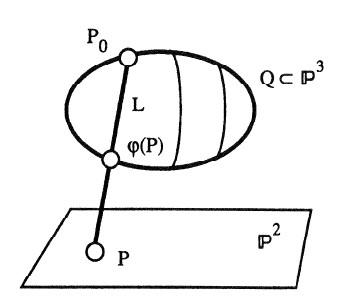
\includegraphics[width=10cm]{57.jpg}\\
			% \caption{初}
		\end{figure}
		
	\section{双有理映射}
		\textbf{定义}\ 取 $V$ 和 $W$ 是 (仿射的或射影的)两个簇,则一个有理映射
		$f:V \dashrightarrow W$是双有理的 (或是一个双有理等价)如果它有一个有理的逆, 即,如果存在有理映射$g: W \dashrightarrow V$使得 $f \circ g=id_{W}$ 且 $f \circ g=id_{V}$
		
		\textbf{命题}\ 在一个有理映射$f: V \dashrightarrow W$上,下列三个条件是等价的:
		\begin{enumerate}[(i)]
			\item $f$是一个双有理等价
			\item $ f $是显性的(见(4.10)),且$f ^{*}: k ( W ) \rightarrow k ( V )$是一个同构
			\item 存在开集$V _{0} \subset V$和$W _{0} \subset W$使得$f$在$V _{0}$上的限制是一个同构 $f : V _{0} \rightarrow W _{0}$
		\end{enumerate}
		
		
		\textbf{证明}\ 像我们在仿射簇中做的那样,我们定义$f^{*}$, 则 (i) $\Longleftrightarrow$ (ii)的证明同(4.11). (iii) $\rightarrow$ (i) 是显然的,因为一个同构 $f : V_{0} \rightarrow W_{0}$ 和它的逆$g = f ^{-1}: W _{0} \rightarrow V _{0}$ 根据定义在$V$和 $W$间都是有理映射.
		
		对(i) $\Rightarrow$ (iii)的证明是富有技巧性的,虽然这是对具体内容无关的: 由假设 (i), 存在逆有理映射$ f : V \dashrightarrow W$ 和 $ g : W \dashrightarrow V ; $ 则取 $ V ^{\prime}=\operatorname{dom} f \subset V $ 和 $\varphi= f _{ |V ^{\prime}}: V ^{\prime} \rightarrow W ,$ 并且同样地取 $W ^{\prime}=\operatorname{dom} g \subset W$ 和 $\Psi= g_{| W ^{\prime}}: W ^{\prime} \rightarrow V .$
		\begin{figure}[H]
			\centering
			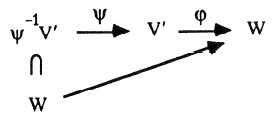
\includegraphics[width=5cm]{58.jpg}\\
			% \caption{初}
		\end{figure}
		
		如上图,所有的箭头都是态射, 且$id_{W_{|\Psi^{-1}}V^{\prime}}=\varphi \circ \Psi$(作为态射)由$ id_{W} = f\circ g $ (作为有理映射)来生成. 因此
		\begin{equation*}
		\varphi(\psi( P ))= P \quad \text {对于所有 } P \in \Psi^{-1} V ^{\prime}
		\end{equation*}
		
		
		现在取$V _{0}=\varphi^{-1} \psi^{-1} V ^{\prime},$和$W _{0}=\psi^{-1} \varphi^{-1} W ^{\prime} ;$则$\varphi: V_{0} \rightarrow \psi^{-1} V ^{\prime}$根据构造是一个态射. 但是, $\psi^{-1} V ^{\prime} \subset W _{0},$ 因为 $P \in \Psi^{-1} V ^{\prime}$ 意味着 $\varphi(\psi( P ))= P ,$ 因此$P \in \Psi^{-1} \varphi^{-1} W ^{\prime}- W_{0}$ . 所以, $\varphi: V _{0} \rightarrow W _{0}$ 是一个态射, 并且$\Psi: W _{0} \rightarrow V _{0}$同样也是一个态射. Q.E.D.
		
		
	\section{有理簇}. 
		(5.8)中讨论的双有理等价概念在代数几何中至关重要.命题中的条件(iii)意味着簇$ V $和$ W $的'内容'是相同的,尽管它们的边缘可能有些不同;使用双有理变换的一个例子是将一个奇异的变量放大以获得一个非奇异的变量,请参见下面的(6.12).接下来将讨论命题5.8的一个特殊情况.
		
		
		\textbf{推论}\  对于给定的簇$V$, 下列两个条件是等价的:
		
		
		(a) 函数域$k ( V )$是对 $k $的一个纯超越扩张,即$k ( V ) \cong k \left( t _{1}, \ldots t _{ n }\right)$ 对某些$n$成立.
		
		
		(b) 存在一个稠密开集$V _{0} \subset V$与稠密开集 $U_{0} \subset \mathbb{A} ^{n}$同构.
		
		
		一个满足上述条件的簇就被称为是有理的.条件(b)事实上是说,$V$可以由$n$个互相独立的变量参数化.这个概念已经隐式地在前文中出现了很多遍(例如 $(1.1), (2.1), (3.11, b), (5.7,II)) .$ 代数几何在数学的其他分支中的大部分基础应用都与有理簇相关.
		
		
	\section{降至超曲面}. 
	
		在第三章末尾讨论诺特正规化的一个简单结论是,对于一个超曲面,每一个簇都是双有理的:首先,因为双有理的判断只依赖于稠密开集, 同时任意一个包含稠密开集的开集都同构于一个仿射簇(根据 (4.13)),因此只需要考虑仿射簇$V \subset \mathbb{A} ^{ n }$.由(3.18),存在元素$y_{1}, . . y_{m+1} \in k [ V ]$ 来生成域扩张$k \subset k ( V ),$并且其中 $y _{1}, \dots y _{ m }$是代数独立的,而$y _{ m +1}$ 在在 $k \left( y _{1}, \dots y _{ m }\right) $上是代数的. 因此这些元素定义了一个态射 $V \rightarrow \mathbb{A} ^{ m +1}$
		,这个态射是关于$V$的一个双有理等价,并且蕴含一个超曲面$V ^{\prime} \subset \mathbb{A} ^{ m +1}$
		
		
	\section{乘法} 
	
	
		如果$V$和 $W$是两个仿射簇,那么存在一个自然的想法, $V \times W$ 是否依然是一个簇:如果 $V \subset \mathbb{A} ^{ n }$ 且 $W \subset \mathbb{A} ^{ m }$ 则$V \times W$ 是是$A ^{ n + m }$的一个子集,且由
		\begin{equation*}
		\left\{\left(\left(\alpha_{1} \ldots \alpha_{n}\right):\left(\beta_{1} \ldots \beta_{m}\right)\right) | f(\underline{\alpha})=0 \forall f \in I(V) \text { 同时 } g(\underline{\beta})=0 ,\forall g \in I(W)\right\}
		\end{equation*}
		给出.
		
		
		显然,$V \times W$ 依然是不可约的. 需要注意到是乘积的Zariski拓扑不是Zariski拓扑的乘积(见\textit{练习5 .10 }). 
		
		
		对于射影簇,情况就变得复杂了; 为了能够定义乘积, 我们需要先判断$\mathbb{P} ^{n} \times \mathbb{P} ^{m}$ 本身是否是一个射影簇. 需要注意到,这个乘积绝对不同构于$\mathbb{P} ^{ n + m }$ (见 \textit{练习5.2, ii}). 为了进行这个判断,我们使用和 (5.7,I)相似的构造思想: 作成一个嵌入 (这被称为'Segre 嵌入')
		\begin{equation*}
		\varphi: \mathbb{P} ^{n} \times \mathbb{P} ^{m} \rightarrow S_{n, m} \subset \mathbb{P}^{ N}, \text {其中 } N=(n+1)(m+1)-1
		\end{equation*}
		
		
		其中$\mathbb{P}^{ N}$是有齐次坐标
		\begin{equation*}
		\left(U_{i j}\right)_{i}=0, \ldots n; j=0,\ldots m
		\end{equation*}
		的一个射影空间.
		
		
		将$ U_{ij} $可以作成下述矩阵
		\begin{equation*}
		\left[\begin{array}{ccc} 
		U _{ 00} & \dots & U _{ 0m } \\
		U _{10} & \dots & \dots \\
		\dots & \dots & U _{ nm }
		\end{array}\right]
		\end{equation*}
		
		
		然后定义$\varphi$ 由 $\left(\left( X _{0}, . . X _{ n }\right),\left( Y _{0}, . . Y _{ m }\right)\right) \mapsto\left( X _{ i } Y _{ j }\right)_{ i =0, \ldots n, j =0, \ldots m}  $.这显然是一个良定义的态射 ,而象$S_{n, m}$ 可以被看作由
		
		\begin{equation*}
		\operatorname{rank}\left[\begin{array}{ccc} 
		U _{00} & \cdots & U _{ 0m } \\
		U _{10} & \cdots & \cdots \\
		\cdots & \cdots & U _{ nm }
		\end{array}\right] \leq 1, \text {即, det }\left|\begin{array}{cc} 
		U _{\text {ik }} & U _{ i l} \\
		U _{ jk } & U _{ j l}
		\end{array}\right|=0 \begin{array}{l}
		\forall i , j =0,\ldots n \\
		\forall k , l=0,\ldots m
		\end{array}
		\end{equation*}
		给出的仿射子簇.
		
		
		下面开始找出逆映射$S _{ n , m } \rightarrow \mathbb{P}^{n} \times \mathbb{P}^{m}$. 对于 $P \in S _{ n , m }$ 至少存在一组 $(i, j)$ 使得 $U_{i j}(P) \neq 0 ;$ 固定这一组 $(i, j),$ 并作成
		\begin{equation*}
		S _{ n , m } \ni P \mapsto\left(\left( U _{0 j }, . U _{ n j}\right),\left( U _{ i 0} \ldots U _{ im }\right)\right) \in \mathbb{P} ^{ n } \times \mathbb{P}^{ m}
		\end{equation*}
		
		
		注意到, $(i, j)$的选取并不影响上述构造, 因为矩阵 $U_{i j}(P)$的秩为 1 并因此矩阵的所有行和所有列都是成比例的.
		
		因此,不能看出如果$V \subset \mathbb{P} ^{ n }$ 且 $W \subset \mathbb{P} ^{m}$ 都是射影簇, 则 $V \times W \subset \mathbb{P}^{n} \times \mathbb{P}^{ m} \cong S _{ n , m } \subset \mathbb{P}^{N}$ 依然是射影簇(见\textit{练习 5.11} ).
		
	\section*{练习}
	
		\subsection{证明一个$ \mathbb{P} ^{1} $上的正规函数是常数函数.(提示:可以使用(5.0)中的方法,假设$f \in k ( \mathbb{P}^{ 1})$在$\mathbb{P} ^{1}$的任何点处都是正规的.在仿射片$\mathbb{A} ^{1}_{(0)}$上应用(4.8,II)并证明$f = p \left( x _{0}\right) \in k \left[ x _{0}\right]$, 在另一个仿射片 $A ^{1}_{(\infty)}$上证明$f = p \left(1 / y _{1}\right) \in k \left[ y _{1}\right] .$现在, 当$p \left(1 / y _{1}\right)$ 是一个多项式时会有怎样的结论?) 并推导对于任意$ m $都不存在非常数的态射 $\mathbb{P}^{1} \rightarrow \mathbb{A} ^{ m }$.}
		
		\textbf{解:}
		
		假设$ f $在$ \mathbb{P}^{1} $上正规,则$ f $在仿射片$\mathbb{A} ^{1}_{(0)}$上正规,$ f \in k[\mathbb{A} ^{1}_{(0)}] \cong k[x_{0}]/I(\mathbb{A} ^{1}_{(0)}) $,$ I(\mathbb{A} ^{1}_{(0)}) =0 $,因此$ f \in k[x_{0}] $,记作$ f = p(x_{0}) $.
		
		同理,$ f $在仿射片$\mathbb{A} ^{1}_{(\infty)}$上正规,则$ f \in k[y_{1}] $.
		
		由$ (5.0) $知,有同构$\mathbb{A} ^{1}_{(0)}\backslash0 \rightarrow \mathbb{A} ^{1}_{(\infty)}\backslash\infty,x_{0} \mapsto y_{1} = \frac{1}{x_{0}} $.
		
		所以$ f = p(\frac{1}{y_{1}} \in k[y_{1}] $,$ p(\frac{1}{y_{1}} $是一个多项式,且只能是0次的,因此$ f $是一个常值函数.
		
		设$ g: \mathbb{P^{1}} \rightarrow \mathbb{A}^{m},g = (g_{1},g_{2},\dots,g_{m}) $,$ g_{i} $是$ \mathbb{P^{1}} $上的正规函数,则$ g_{i} $是常值函数,进而$ g $是常值映射.
		
		
		\subsection{$\mathbb{P} ^{3}$上的二次曲面.}
		
		
		\begin{enumerate}[(i)]
			\item 证明(5.10)中$\mathbb{P} ^{1} \times \mathbb{P} ^{1}$的Segre嵌入给出了$\mathbb{P} ^{1} \times \mathbb{P} ^{1}$到
			\begin{equation*}
			S_{1,1}=Q:\left(X_{0} X_{3}=X_{1} X_{2}\right) \subset \mathbb{p}^{3}
			\end{equation*}
			的一个同构.
			\item 在$\mathbb{P} ^{1} \times \mathbb{P} ^{1}$上,两族直线$\{p\} \times \mathbb{P} ^{1}$和$\mathbb{P} ^{1} \times\{p\}$在$ Q $中的象是什么?并找出$\mathbb{P} ^{1} \times \mathbb{P} ^{1}$中的不相交直线,进而证明$\mathbb{P} ^{1} \times \mathbb{P} ^{1} \not \neq \mathbb{P} ^{2}$.
			(这跟解析几何中提到的二次曲面的直纹性是一致的.)
			\item 证明$ Q $中有两条直线过点 $P=(1,0,0,0)$, 并且这两条直线的补集$ U $恰好是$\mathbb{A} ^{1} \times \mathbb{A} ^{1}$在Segre嵌入下的象.
			\item 证明在射影$\pi_{|Q} : Q \rightarrow \mathbb{P} ^{2}$(即(5.7,II)中的记法)下,$ U $同构地映到$\mathbb{A}^{2}$的一个镜像,同时过$ P$的两条直线映到$\mathbb{P} ^{2}$上.
			\item 使用(5.7,II)的记号,找出$ \operatorname{dom} \pi \text { 和} \operatorname{dom} \varphi $,并给出关于$\pi$ 和 $\varphi$奇异性的几何解释.
		\end{enumerate}
	
		\textbf{解:}
		\begin{enumerate}[(i)]
			\item 建立映射$ \varphi: \mathbb{P}^{1} \times \mathbb{P}^{1} \mapsto S_{1,1} $
			\begin{equation*}\left(a_{0}, a_{1}\right) \times\left(b_{0}, b_{1}\right) \longmapsto\left(\begin{array}{ll}
			a_{0} b_{0} & a_{0} b_{1} \\
			a_{1} b_{0} & a_{1} b_{1}
			\end{array}\right)\end{equation*}
			$ S_{1,1} $中点的坐标$\left(x_{0}, x_{1}, x_{2}, x_{3}\right)=\left(a_{0} b_{0}, a_{0} b_{0}, a_{1} b_{0}, a_{1} b_{1}\right)$,满足$ x_{0}x_{3} = x_{1}x_{2} $
			
			$ \varphi $的逆映射为$ S_{1,1} \mapsto \mathbb{P}^{1} \times \mathbb{P}^{1} $
			\begin{equation*}\left\{\left(x_{0}, x_{1}, x_{2}, x_{3}\right) | x_{0} x_{3}=x_{1} x_{2}\right\} \mapsto\left(\left(x_{0}, x_{1}\right),\left(x_{0}, x_{3}\right)\right) \in  \mathbb{P}^{1} \times \mathbb{P}^{1}\end{equation*}
			
			\item 设$ P $的坐标为$ (P_{0},P_{1}) $,则$ \{P\} \times \mathbb{P}^{1} $在$ S_{1,1} $中的象是
			\begin{equation*}\begin{array}{l}
			\left(x_{0}, x_{1}, x_{2}, x_{3}\right)=\left(p_{0}b_{0}, p_{0}b_{1}, p_{1}b_{0}, p_{1} b_{1}\right) \\
			x_{0}:x_{2}=x_{1}: x_{3}=P_{0}: P_{1} \Rightarrow\left\{\begin{array}{l}
			P_{1} x_{2}=P_{1}x_{0} \\
			P_{0} x_{3}=P_{1}x_{1}
			\end{array}\right.
			\text{是$ Q $中的一条直线}
			\end{array}\end{equation*}
			
			同理$ \mathbb{P}^{1} \times \{P\} $在$ S_{1,1} $中的象是
			\begin{equation*}\begin{array}{l}
			\left(x_{0}, x_{1}, x_{2}, x_{3}\right)=\left(a_{0}p_{0}, a_{0}p_{1}, a_{1}p_{0}, a_{1} p_{1}\right) \\
			x_{0}:x_{2}=x_{1}: x_{3}=P_{0}: P_{1} \Rightarrow\left\{\begin{array}{l}
			P_{1} x_{1}=P_{1}x_{0} \\
			P_{0} x_{3}=P_{1}x_{2}
			\end{array}\right.
			\text{是$ Q $中的一条直线}
			\end{array}\end{equation*}
			$ \forall a \neq b,  \{a\} \times \mathbb{P}^{1} $和$ \{b\} \times \mathbb{P}^{1} $是两条不相交直线.
			
			\item 过$ P(1,0,0,0) $的直线在$ \mathbb{P}^{1} \times \mathbb{P}^{1} $中的原象是$ \{q\} \times \mathbb{P}^{1} $或$ \mathbb{P}^{1} \times  \{q\}$.所以过$ P $的直线是$ (p_{0}b_{0}, p_{0}b_{1}, p_{1}b_{0}, p_{1} b_{1}) $或$ (a_{0}p_{0}, a_{0}p_{1}, a_{1}p_{0}, a_{1} p_{1}) $形式.$ P $的第一个坐标不为$ 0 $,所以$ q_{0} \neq 0,q_{1} = 0 $,两条直线为$ (p_{0}b_{0}, p_{0}b_{1}, 0,0 )$和$ (a_{0}p_{0},0, a_{1}p_{0}, 0) $都过点$ P $.
			
			这两条直线在$ \mathbb{P}^{1} \times \mathbb{P}^{1} $中的原象是$ (q_{0},0)\times \mathbb{P}^{1} $和$ \mathbb{P}^{1} \times (q_{0},0) $,它们的补集为
			\begin{equation*}\mathbb{P}^{1} \times \mathbb{P}^{1} \backslash \{(1,0)\times \mathbb{P}^{1},\mathbb{P}^{1} \times(1,0)\}\end{equation*}
			即$ \mathbb{A}^{1} \times \mathbb{A}^{1} $
			
			\item \begin{equation*}\begin{array}{l}
			U=\left\{\left(a_{0} b_{0}, a_{0} b_{1}, a_{1} b_{0}, a_{1} b_{1}\right) |\left(a_{0}, a_{1}\right) \neq(1,0),\left(b_{0},b_{1}\right) \neq(1,0)\right\} \\
			\left.\pi\right|_{U}=\left\{\left(a_{0} b_{0}, a_{1} b_{0}, a_{1} b_{1}\right) | a_{1} \neq 0, b_{1} \neq 0\right\}=\left\{\left(\frac{a_{0}}{a_{1}}, \frac{b_{0}}{b_{1}}, 1\right)\right\} \cong \mathbb{A}^{2}
			\end{array}\end{equation*}
			过$ P $的两条直线在$ \pi $下的象为$ \{(q_{0}b_{1},0,0),(0,a_{1}q_{0},0)\}=\{(1,0,0),(0,1,0)\} \in \mathbb{P}^{2} $
			
			\item 
			\begin{equation*}\operatorname{dom} \pi=\mathbb{P}^{3}\backslash\{(1,0,0,0)\} \quad \operatorname{dom} \varphi= \mathbb{P}^{2} \backslash\{(x_{1}, x_{3}, 0)\}\end{equation*}
		\end{enumerate}
		\subsection{下列的几个表达中,哪些定义了一个建立在两个具有合适维数$(n, m=1 \text { 或 } 2) $的射影空间的有理映射,即$\varphi: \mathbb{P} ^{n} \rightarrow \mathbb{ P} ^{m}$?对于每一种表达确定$ dom \varphi $和$ \varphi $是否时双有理的,如果是双有理的则写出逆映射.}
		\begin{enumerate}[(a)]
			\item $(x, y, z) \mapsto(x, y)$ 
			\item $(x, y) \mapsto(x, y, 1)$ 
			\item $(x, y) \mapsto(x, y, 0)$
			\item $(x, y, z) \mapsto(1 / x, 1 / y, 1 / z)$ 
			\item $(x, y, z) \mapsto\left(\left(x^{3}+y^{3}\right) / z^{3}, y^{2} / z^{2}, 1\right)$
			\item  $(x, y, z) \mapsto\left(x^{2}+y^{2}, y^{2}, y^{2}\right)$
		\end{enumerate}
	
		\textbf{解:}
		\begin{enumerate}[(a)]
			\item 显然是一个有理映射,但它不是双有理的.
			\item 是有理映射同时也是双有理的,它的逆映射是$(x, y,1) \mapsto(x, y)$. 
			\item 在射影簇上$ (x, y, 0) $是没有定义的,因此这不是一个有理映射.
			\item 是有理映射同时也是双有理的,逆映射是$(x, y, z) \mapsto(1 / x, 1 / y, 1 / z)$ 
			\item 是有理映射但不是双有理的 
			\item 是有理映射但不是双有理的
		\end{enumerate}
	
		\subsection{三阶有理正规曲线(如(5.7,I))是由三个二次曲面定义的,即曲线$C \subset P ^{3}$ 且$C=Q_{1} \cap Q_{2} \cap Q_{3},$,其中}
			\begin{equation*}
			Q _{1}:\left( XZ = Y ^{2}\right), Q _{2} :( XT = YZ ), Q _{3}:\left( YT = Z ^{2}\right)
			\end{equation*}
		这条曲线被称为\textit{三次挠线}, 其中\textit{挠}代表这不是一个平面曲线. 验证对于任意两个二次曲面$Q_{i}, Q_{j},$ 它们的交$Q _{ i } \cap Q _{ j }= C \cup \ell_{ i j},$ 其中 $\ell_{ i j}$ 是一条确定的直线. 因此在3维空间中,这条曲线不是任两个二次曲面的交.
		
		\textbf{解:}
		
		$
		\left\{
		\begin{aligned}
		XZ = Y ^{2} \\
		XT = YZ\\
		\end{aligned}
		\right.
		\Longleftrightarrow
		\left\{
		\begin{aligned}
		YT = Z ^{2} \\
		XT^{2} = Z^{3}\\
		\end{aligned}
		\right.
		$
		即$Q _{ 1 } \cap Q _{ 2 }= C \cup \ell_{ 12}$,其中$\ell_{ 12}: XT^{2} = Z^{3}  $
		
		$
		\left\{
		\begin{aligned}
		XT = YZ \\
		YT = Z ^{2}\\
		\end{aligned}
		\right.
		\Longleftrightarrow
		\left\{
		\begin{aligned}
		XZ = Y ^{2} \\
		XT^{2} = Z^{3}\\
		\end{aligned}
		\right.
		$
		即$Q _{ 2 } \cap Q _{ 3 }= C \cup \ell_{ 23}$,其中$\ell_{ 23}: XT^{2} = Z^{3}  $
		
		$
		\left\{
		\begin{aligned}
		XZ = Y ^{2} \\
		YT = Z ^{2}\\
		\end{aligned}
		\right.
		\Longleftrightarrow
		\left\{
		\begin{aligned}
		XT = YZ \\
		XT^{2} = Z^{3}\\
		\end{aligned}
		\right.
		$
		即$Q _{ 1 } \cap Q _{ 3 }= C \cup \ell_{ 13}$,其中$\ell_{ 13}: XT^{2} = Z^{3}  $
		
		因此,得证这条曲线不是任两个二次曲面的交.
	
		\subsection{取 $Q_{1}:\left(X Z=Y^{2}\right)$和 $F:\left(X T^{2}-2 Y Z T+Z^{3}=0\right)$; 证明 $C=Q_{1} \cap F$是习题 5.4中提到的三次挠线. }
		
		\textbf{解:}
		显然,$ X T^{2}-2 Y Z T+Z^{3}=0 \Longleftrightarrow XZT^{2}-2 Y Z^{2} T+Z^{4}=0$,代入$ X Z=Y^{2} $则有$ (YT - Z ^{2})^{2} = 0 \Longleftrightarrow YT = Z ^{2} $.
		
		同理,由$ Q_{1} $和$ F $可推出$ XT = YZ $.
		
		综上则有$ Q_{1} \cap F \Longrightarrow  Q_{1} \cap Q_{2} \cap Q_{3}$.
		
		反之,$ Q_{2} \cap Q_{3} \Longrightarrow F$.
		
		综上,有$Q_{1} \cap F \Longleftrightarrow  Q_{1} \cap Q_{2} \cap Q_{3}  $,则得证.
%			
		\subsection{取 $C \subset \mathbb{P} ^{3}$是由 $C = Q _{1} \cap Q _{2}$定义的不可约曲线,其中$Q _{1}:\left( T X = q _{1}\right), Q _{2}:\left( TY = q _{2}\right),$ 而 $q _{1}, q _{2}$ 是$X , Y , Z$构成的二次型. 证明由$( X , Y , Z , T ) \mapsto( X , Y , Z )$定义的射影$\pi: \mathbb{P} ^{3} \dashrightarrow \mathbb{P} ^{2}$可以限制成 $ C $到由$X q_{2}= Yq_{1}$给出的平面曲线$D \subset\mathbb{ P} ^{2}$ 的一个同构.}
	
%			
		\subsection{取 $\varphi: \mathbb{P} ^{1} \rightarrow \mathbb{P} ^{1}$是一个同构; 找出$\varphi$ 作为 $\mathbb{P} ^{1} \times \mathbb{P} ^{1} \times Q \subset \mathbb{P} ^{3}$的一个子簇的图像. 设 $\varphi: \mathbb{P} ^{1} \rightarrow P ^{1}$是一个 2 -到-1 的映射并由$(x, y) \mapsto\left(x^{2}, y^{2}\right)$给出,再找出$\varphi$的图像}
%			
%		
		\subsection{证明任意不可约二次曲线$Q \subset P ^{n+1}$ 是有理的; 即, 像(5.7. II)的图片那样, 如果$P\in Q$是一个非奇异点,则 $\mathbb{P} ^{n+1}$ 到$\mathbb{P} ^{n}$的线性射影将诱导出一个双有理映射$Q \dashrightarrow \mathbb{P} ^{n}$. }
%			
%			
		\subsection{对下列的每一个平面曲线,写出3标准仿射片,并判断曲线和3坐标轴的交点:
			(a) $y^{2} z-x^{3}+2 x^{2}+b z^{3}$
			(b) $x^{2} y^{2}+x^{2} z^{2}+y^{2} z^{2}=2 x y z(x+y+z)$
			(c) $x z^{3}-\left(x^{2}+z^{2}\right) y^{2}$}
%			
%			
		\subsection{ (i) 证明两个不可约代数集的乘积依然是不可约的. (提示:对所有子集$w \in W$,子集$V \times\{w\}$都是不可约的, 如果给出了$V \times W = U _{1} \cup U _{2}$, 则需要考虑子集$ W _{ i }=\{ w \in W | V \times\{ w \} \subset U _{ i }\} \text{其中} i =1,2$}
			
				
			(ii)描述在$\mathbb{A}^{2}=\mathbb{A}^{1} \times \mathbb{A}^{1}$上拓扑的闭集,这个拓扑是两个分式上Zariski拓扑的乘积; 并找出不同于上述形式的$\mathbb{A}^{2}$上Zariski拓扑的闭集.
			
		\textbf{解:}
		
		$ (i) $首先证明两个不可约代数集的乘积依然是代数集
		
		设$ V,W $是两个代数集,$ V \times W = \{(\alpha_{1},\ldots,\alpha_{n},\beta_{1},\ldots,\beta_{m}) | f(\alpha) = 0, \forall f \in I(V),g(\beta) = 0 ,\forall g \in I(W) \}, V \subset \mathbb{A}^{n},W \subset \mathbb{A}^{m}$
		\begin{equation*}\begin{aligned}
		&\begin{array}{l}
		I(V \times W)\supset \left\{f^{2}+g^{2}|f\in I( v), g \in I(w)\}, f^{2}+g^{2} \in k\left[x_{1}, \dots x_{n}, y_{1}, \dots y_{m}\right]\right. \\
		V(I(V \times W)) \subset V\left\{f^{2}+g^{2} | f \in I(v), g \in I(w)\right\}=V \times W
		\end{array}\\
		&\text{又因为} V \times W \subset V(I(V \times W)),\text { 因此} V \times W=V(I(V \times W))
		\end{aligned}\end{equation*}
		因此$ V \times W $是代数集.
		
		对于$ w \in W $,子集$ V \times \{w\} $是不可约的,如果$ V \times W = U_{1} \cup U_{2} $,$ U_{1} , U_{2}  $都是代数集,则考虑子集$ W_{i} = \{w \in W | V \times \{w\} \subset U_{i}\},i = 1,2 $,有$ W_{1} \cup W_{2} = W $且$ V \times W_{1} = U_{1}, V \times W_{2} = U_{2} $是代数集.
		
		则$ W_{1},W{2} $是代数集,与$ W $可约矛盾.
		
		如果$ W_{i} ,i = 1,2$不是代数集,则 $W_{i} \varsubsetneqq V\left(I\left(W_{i}\right)\right),V \times W_{i}\varsubsetneqq \{(\alpha_{1},\ldots,\alpha_{n},\beta_{1},\ldots,\beta_{m})|f(\alpha) = 0, \forall f \in I(V),g(\beta) = 0 ,\forall g \in I(W_{i})\} = V \times V(I(W_{i}))$,这与$ (5.11) $中的集合乘积定义矛盾.
		
		$ (ii) $ $ \mathbb{A}_{2} = \mathbb{A}_{1} \times \mathbb{A}_{1} $,两个分式上$ Zariski $拓扑的乘积
		
		闭集$ V{I} \times V(J),I,J \in k[X] $
		
		$ f = X - Y \in k[X,Y],V(f) = (X,X) \in  \mathbb{A}_{2}$是无限集,而$ V(I),V(J) $都是有限集,$ V(I) \times V(J) $也是有限集.
		
		
		\subsection{(a) 如果$\mathbb{A}^{n}_{(0)}$ 和 $\mathbb{A}^{m}_{ ( 0 )}$分别是$\mathbb{P}^{n}$和$\mathbb{P}^{m}$的标准仿射片,验证(5.11)中的Segre 嵌入将$\mathbb{A} ^{ n }(0) \times \mathbb{A} ^{ m }(0)$ 同构地映射到簇$S_{n, m} \subset \mathbb{P} ^{n}$上的一个仿射片, 称作 $s_{(0)} \subset \mathbb{A} ^{N}$, 并且$\mathbb{A}^{N}$的$ n $个坐标将限制在$X_{1} \ldots X_{n}, Y_{1} \ldots Y_{m}$上 }
			(b)如果$V \subset \mathbb{P} ^{ n }$ 且 $W \subset \mathbb{P} ^{ m }$,证明乘积 $V \times W$ 是 $\mathbb{P} ^{ n } \times \mathbb{P} ^{ m }= S _{ n , m } \subset\mathbb{ P} ^{ N }$的一个射影子簇 (提示:根据(5.11),仿射片的乘积$V (0) \times W _{(0)} \subset \mathbb{A }^{n+m}$是一个由多项式定义的子簇;证明每一个仿射片的乘积都是$U _{ i j }$上齐次多项式在$\mathbb{A} ^{ n + m } \propto S _{(0)}$ 上的限制).
			
		\textbf{解:}
		$ (a) $ 验证 $A_{(0)}^{n}=\left(1, x_{1}, x_{2}, \ldots, x_{n}\right)$
		$A_{(0)}^{m}=\left(1, y_{1}, y_{2}, \ldots, y_{m}\right)$
		\begin{equation*}\varphi : A_{(0)}^{n} \times A_{(0)}^{m} \mapsto \left(\begin{array}{ccccc}
		1 & y_{1} & y_{2} & \cdots & y_{m} \\
		x_{1} & x_{1} y_{1} & x_{1} y_{2} & \dots & x_{1} y_{m} \\
		\vdots & \vdots & & \\
		x_{n} & x_{n} y_{1} & x_{n} y_{2} & \cdots & x_{n} y_{m}
		\end{array}\right)
		\text{是$ \mathbb{P}^{n} $中的仿射片,记作$ S_{(0)} $}\end{equation*}
		$ \mathbb{A}^{N} $的$ N $个坐标限制在$x_{1} \dots x_{n}, y_{1} \dots y_{m}$以及$ mn $个$ x_{i}y_{j} $上.
		
		$ (b) $
		\begin{equation*}\begin{array}{l}
		\mathbb{P} ^{n}=\bigcup_{i=0}^{n} A_{(i)}^{n} \quad \mathbb{P} ^{m}=\bigcup_{j=0}^{m} A_{(j)}^{m}\\
		V_{i} = V \cap A_{(i)}^{n},W_{j} = W \cap A_{(j)}^{m},V_{i} \times V_{j} \subset A^{m+n} \cong S_{(0)}\\	
		V_{i}=V \cap A^{n}_{(i)}=\left\{\left(X_{1}, \cdots X_{i-1},1, X_{i +1}, \cdots X_{n}\right) | f(X)=0, \forall f \in I(V)\right\} \\
		W_{j}=W \cap A_{(j)}^{m}=\left\{\left(Y_{1}, \ldots Y_{i-1}, 1, Y_{j+1}, \ldots, Y_{m}\right) | g(Y)=0, \forall g \in I(W)\right\}\end{array}
		\end{equation*}
		\begin{equation*}
		V_{i} \times W_{j} =  \left(\begin{array}{cccccccc}
		x_{1}y_{1}&x_{1}y_{2}&\cdots&x_{1}y_{j-1}&x_{1}&x_{1}y_{j+1}&\cdots&x_{1}y_{m} \\
		x_{2}y_{1}&x_{2}y_{2}&\cdots&x_{2}y_{j-1}&x_{2}&x_{2}y_{j+1}&\cdots&x_{2}y_{m} \\
		\cdots & &\cdots& & & &\cdots&  \\
		y_{1}&y_{2}&\cdots&y_{j-1}&1&y_{j+1}&\cdots&y_{m} \\
		\cdots & &\cdots& & & &\cdots&  \\	
		x_{n}y_{1}&x_{n}y_{2}&\cdots&x_{n}y_{j-1}&x_{n}&x_{n}y_{j+1}&\cdots&x_{n}y_{m} \\
		\end{array}\right)\end{equation*}
		是$ V \times W$的一个仿射片.
		
		当$ i $取遍$ 0,1,\cdots,n $,$ j $取遍$ 0,1,\cdots,m $,则$ V_{i} \times W_{j} $得到$ N+1 $个仿射片,覆盖$ V \times W$.
			
			
		\subsection{取$C$ 是(5.0)中的二次曲线, 证明在 $C$上任意正规函数 $f$ 都是常数. 证明可以按照下述步骤:}
			\begin{enumerate}[Step 1]
			\item 在仿射片$C_{(0)}$上应用(4.8,II),记 $f=p(x, y) \in K [x, y]$ 
			\item 减去$y^{2}-x^{3}-a x-b$的一个合适的倍数,并假设$p(x, y)=q(x)+y r(x),$ 其中 $q, r \in k[x]$
			\item 在仿射片$C_{(\infty)}$上应用(4.8,11) 并给出
			\begin{equation*}
			f=q\left(x_{1} / z_{1}\right)+\left(1 / 2_{1}\right) r\left(x_{1} / 2_{1}\right) \in k\left[C_{(\infty)}\right]
			\end{equation*}
			并因此存在一个多项式$S\left(x_{1}, z_{1}\right)$使得
			\begin{equation*}
			q\left(x_{1} / z_{1}\right)+\left(1 / z_{1}\right) r\left(x_{1} / z_{1}\right)-s\left(x_{1}, z_{1}\right)
			\end{equation*}
			\item 约掉分母并根据$k \left[ C _{(\infty)}\right]= k \left[ x _{1}, z_{1}\right] / g ,$ 其中$g=z_{1}-x_{1}^{3}-a x_{1} z_{1}^{2}-b z_{1}^{3},$ 来推出$k \left[ x _{1}, z _{1}\right]$上的多项式恒等式
			\begin{equation*}
			Q _{ m }\left( x _{1}, z _{1}\right)+ R _{ m -1}\left( x _{1}, z _{1}\right)= S \left( x _{1}, z _{1}\right) z _{1}^{ m }+ A \left( x _{1}, z _{1}\right) g
			\end{equation*}
			,其中$Q _{ m }$ and $R _{ m -1}$都是齐次且次数已知的.
			\item 现在如果记$S=S^{+}+S^{-}$ 而$A=A^{+}+A^{-}$来将其分成分别是偶数和奇数阶的项,需要注意$g$ h只具有偶数阶的项, 如果$m$是偶数,则恒等式可以分成:
			\begin{equation*}
			Q _{ m }= S ^{+} z _{1}^{ m }+ A ^{-} g \quad \text { 和} \quad R _{ m -1}= S ^{-} z _{1}^{ m }+ A ^{+} g
			\end{equation*}
			而如果$m$是奇数,那么同样有类似的表达. 
			\item $Q_{m}$是$m$次齐次的, 因此 $A ^{-} g$的次数 $\geq m$; 考虑 $A ^{-} g$中次数最小的项,并证明 $Q _{ m }$是可以被 $z _{1}$整除的.对$R_{m-1}$进行同样的操作. 取$m$ 为Step 4中允许的最小值,就能证明$q(x)$是0次的,同时 $r(x)=0$
		\end{enumerate}
	
	
	
	
		\subsection{\textbf{Veronese曲面}\ 考虑由$( X , Y , Z ) \mapsto \left( X ^{2}, XY , XZ , Y ^{2}, YZ , Z ^{2}\right) $给出的嵌入$\varphi: \mathbb{P} ^{2} \rightarrow \mathbb{P} ^{5}$ ,写出定义象 $S =\varphi\left( \mathbb{P} ^{2}\right)$的方程组,并证明 $\varphi$是一个同构 (这一步可以通过写出逆同构的方程组来进行). 证明 $\mathbb{P} ^{2}$中的直线在$\mathbb{P} ^{5}$上表现为二次曲线,并且$\mathbb{P}^{2}$上的二次曲线在$\mathbb{P} ^{5}$上表现为四次挠线(见(5.7)).对于任意直线$\ell \subset P ^{2}$,记$\pi( L ) \subset P ^{5}$是由二次曲线 $\varphi (\ell)$张成的射影平面. 证明所有 $\ell \subset P ^{2}$对应的 $\pi(\ell)$的并是三次超曲面$\Sigma \subset \mathbb{P} ^{5} .$ (提示: 像(5.7)和(5.11)那样.)}
		
\chapter{切空间,非奇异性与维数}
\section{超曲面的非奇异点}
假设$f\in k[X_{1},...,X_{n}]$是不可约的,$f\notin k$,然后令$V=V(f)\subset \mathbb{A}^{n}$;令$P=(a_{1},...,a_{n})\in V$,令$ l $是过$ P $点的直线.因为$P\in V$,显然$ P $是$f|_{l}$的根.


\textbf{问题:}\ 什么时候点$ P $是$f|_{l}$的重根?


\textbf{答案:}\ 当且仅当$ l $包含于仿射线性子空间


\begin{center}
	$T_{P}V:(\Sigma_{i}\frac{\partial f}{\partial X_{i}}(P)\cdot(X_{i}-a_{i})=0)\subset \mathbb{A}^{n}$
\end{center}


称作在$ P $点的$ V $的切空间.


\begin{center}
	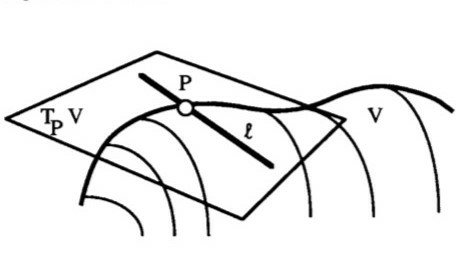
\includegraphics{pic.png}
\end{center}


为了证明这一结论,参数化$ l $


\begin{center}
	$l:X_{i}=a_{i}+b_{i}T$
\end{center}


其中$P=(a_{1},...,a_{n})$和$(b_{1},...,b_{n})$是$ l $的坡度向量和方向向量.则$f|_{l}=f(...,a_{i}+b_{i}T,...)=g(T)$是$ T $中的多项式,而且我们知道$ (T=0) $是$ g $的一个根.因此


\begin{center}
	0是$ g $的重根$\iff$ $\frac{\partial g}{\partial T}(0)=0$
\end{center}


即,


\begin{center}
	$\iff$ $\Sigma_{i}b_{i}\frac{\partial f}{\partial X_{i}}(P)=0 \iff l\subset T_{P}V$
\end{center}


\textbf{定义}\ $P\in V \subset \mathbb{A}_{n}$是$ V $中的非奇异点,如果对于一些$ i $有$\frac{\partial f}{\partial X_{i}}\ne 0$;否则$ P $是奇异点,或者说在$ V $上具有奇异性.


显然,如果$ P $是非奇异的,那么$T_{P}V$是$\mathbb{A}^{n}$的$ (n-1) $维仿射子空间,而若$P\in V$是奇异的,则有$T_{P}V$= $\mathbb{A}^{n}$.


\section{一些注解}
(a)上面提到的求导运算$\frac{\partial f}{\partial X_{i}}(P)$是形式化的代数运算;不涉及更深入的微积分原理.


(b)假设$k=\mathbb{R}$或$\mathbb{C}$,同时$\frac{\partial f}{\partial X_{i}}(P)\ne 0$;不妨取$i=1$;则由$(X_{1},...,X_{n})\mapsto (f,X_{2},...,X_{n})$定义的映射$p:\mathbb{A}^{n} \longrightarrow \mathbb{A}^{n}$在$ P $点有非零的雅克比行列式,故由反函数定理,存在邻域$P\in U \subset \mathbb{A}^{n}$使得$p|_{U}: U\rightarrow p(U)\subset \mathbb{A}^{n}$是邻域$ U $的微分同胚映射(与$\mathbb{R}^{n}$或$\mathbb{C}^{n}$相同的拓扑);即,$p|_{U}$ 是双射,$ p $与$p^{-1}$是有实变量或复变量的可微函数.换句话说,$(f,X_{2},...,X_{n})$在靠近$ P $点的$\mathbb{A}^{n}$上形成了一个新的可微坐标系;这意味着$V:(f=0)$ 中$ P $点的一个邻域和$\mathbb{A}^{n-1}$中的一个开集在坐标$(X_{2},...,X_{n})$下是微分同胚的.这样,在非奇异点$ P` $附近,$ V $是以$(X_{2},...,X_{n})$作为局部参数的流形.


\section{命题}
$V_{nonsing}=\{P\in V |$P是非奇异的$\}$在Zariski拓扑下是$ V $的稠密开集.


\textbf{证明}\ $V_{nonsing}$的补集是奇异点的集合$V_{sing}$,由$\frac{\partial f}{\partial X_{i}}(P)=0$(对于所有$ i $值)定义,即


\begin{center}
	$V_{sing}=V(f,\frac{\partial f}{\partial X_{1}},...,\frac{\partial f}{\partial X_{n}})\subset \mathbb{A}^{n}$
\end{center}


它在Zariski拓扑下是闭集.由于V是不可约的(由3.11,a),为了证明开集$V_{nonsing}$是稠密的,我只需要证明它是非空的(由命题4.2);反证法,假设它是空集,即,假设$V=V(f)=V_{sing}$.那么$\frac{\partial f}{\partial X_{1}}$的多项式就必须在$ V $上为0,因此(又由3.11)它们必须在$k[X_{1},...,X_{n}]$上可被$ f $除尽;但是作为$X_{i}$上的多项式,$\frac{\partial f}{\partial X_{1}}$的次数必须严格小于$ f $,所以$ f $整除$\frac{\partial f}{\partial X_{1}}$意味着实际上作为一个多项式$\frac{\partial f}{\partial X_{1}}=0$ .在$\mathbb{C}$上,很明显只有$X_{i}$ 不在$ f $里出现,这才可能,而且如果对所有$ i $都成立,那么$ f $就是$\mathbb{C}$上的常数了,这是可以被排除的.在一般的域$ k $上,$\frac{\partial f}{\partial X_{1}}=0$只可能在$ f $是$X_{i}$中的不可分的多项式时成立,即,$ char\ k=p $,且$X_{i}$只在$ f $中以$ p $次幂$X_{i}^{p}$的形式出现.如果对于所有i, 这点都成立,那么由(3.16)中的论证,$ f $是$k[X_{1},...,X_{n}]$中的$ p $次幂项;这与$ f $是不可约的矛盾.证毕.


\section{切空间}
\textbf{定义.}\ 令$V\subset \mathbb{A}^{n}$是一个子簇,$V\ni P=(a_{1},...,a_{n})$.对任意$f\in k[X_{1},...,X_{n}]$,有


\begin{center}
	$f_{p}^{(1)}=\Sigma_{i}\frac{\partial f}{\partial X_{i}}(P)(X_{i}-a_{i})$
\end{center}


这是一个仿射线性多项式(即,线性加常数),$ f $在$ P $点的"一阶部分".现在由下式定义$ V $在$ P $点的切空间


\begin{center}
	$T_{P}V = \bigcap(f_{p}^{(1)}=0)\subset \mathbb{A}^{n}$
\end{center}


这个交集在所有$f\in I(V)$上出现.


\section{命题}
由$P\mapsto dim T_{P}V$定义的函数$V\rightarrow \mathbb{N}$是上半连续的(在$ V $的Zariski拓扑上).换句话说,对于任何整数$ r $,子集


\begin{center}
	$S(r) = \{P\in V|dim T_{P}V\geqslant r\} \subset V$
\end{center}


是闭集.


\textbf{证明}\
令$(f_{1},...,f_{m})$是$ I(V) $的生成元集;显然对于任何$g\in I(V)$,$ g $的线性部分$g_{P}^{(1)}$是$f_{i}$的的线性部分的线性组合,所以$T_{P}V$的定义简化为


\begin{center}
	$T_{P}V = \bigcap^{m}_{i=1}(f_{i,P}^{(1)}=0)\subset \mathbb{A}^{n}$
\end{center}


然后由基础线性代数,


\begin{center}
	$P\in S(r) \Longleftrightarrow$矩阵$(\frac{\partial f_{i}}{\partial X_{j}}(P))_{i=1,....,m,j=1,....,n}$有秩$\leqslant n-r \Longleftrightarrow$每一个$(\frac{\partial f_{i}}{\partial X_{j}}(P))_{i,j}$的子式 $(n-r+1)\times (n-r+1)$都为$ 0 $.
\end{center}


现在矩阵的每个元素$\frac{\partial f_{i}}{\partial X_{j}}(P)$是$ P $的一个多项式函数;这样每一个子式是一个多项式构成的矩阵的行列式,而它本身也是一个多项式.因此$S(r)\subset V\subset \mathbb{A}^{n}$是一个代数集.证毕.


\section{推论-定义}
存在着整数$ r $和稠密开子集$V_{0}\subset V$使得


\begin{center}
	$dim T_{P}V =r$对于任意$P\in V_{0}$,且$dim T_{P}V\geqslant r$对于任意$P\in V$.
\end{center}


定义$ P $的维数为$ r $,记做$dim V= r$;称$P\in V$是非奇异的如果$dim T_{P}V = r$,称$P\in V$是奇异的如果$dim T_{P}V > r$.一个簇$ V $是非奇异的如果它在每一点$P\in V$都是非奇异的.


\textbf{证明}.\ 令$r = min\{dim T_{P}V\}$, 那么显然


\begin{center}
	$S(r-1) = \varnothing,S(r) = V$, 且$S(r+1)\subsetneq V$;
\end{center}


因此$S(r)\backslash S(r+1)=\{P\in V|dim T_{P}V = r\}$是非空开的.证毕.


\section{ }
由命题6.3如果$V = V(f)\subset \mathbb{A}^{n}$是由一些非常数多项式$ f $定义的超曲面,那么$dim V = n-1$.另一方面,对于一个超曲`面,$k[V]=k[X_{2},...,X_{n}]/(f)$,因此,假定$ f $以一种非平凡的方式涉及$X_{1}$,$ V $的函数域就是如下形式


\begin{center}
	$k(V)=k(X_{2},...,X_{n})[X_{1}]/(f)$
\end{center}


这就是说,它是从$ k $加入$ n-1 $个代数独立的元素,然后进行本原代数扩张得到的.


\textbf{定义}\ 如果$k\subset K$是一个域扩张,$ K $在$ k $上的超越次数,就是$ K $在$ k $上代数独立的元素的最大数.它表示为$tr\ deg_{k} {K}$.


这个关于域扩张$K/k$的超越次数的基本理论,形式上和向量空间的维数的理论相似:给定$\alpha_{1},...,\alpha_{m}\in K$,我们知道它们在$ k $上代数独立意味着什么(见3.13);它们跨越了扩张的超越部分如果$K/k(\alpha_{1},...,\alpha_{m})$是代数的;而且它们形成了超越基如果它们是代数独立的.那么这个理论就很简单了:一个超越基是一个极大代数独立集,和一个极小生成集,$ K/k $的任意两组超越基有着相同个数的元素.


因此对于一个超曲面$V\subset\mathbb{A}^{n}$,$dim V = n-1 = tr\ deg_{k}k(V)$.这一章的剩下部分是要通过减少到一个超曲面的情况来证明等式$dim V = tr\ deg_{k}k(V)$对于所有变量都成立.首先需要说明对于簇的一点$P\in V$,切空间$T_{P}V$是$P\in V$处邻域的一个固有性质.


\section{$T_{P}V$的本质}
从现在开始,给定$P = (a_{1},...,a_{n})\in V\subset \mathbb{A}^{n}$,采用新坐标$X_{i}' = X_{i}-a_{i}$把$ P $点变为原点,然后设$P = (0,...,0)$.那么$T_{P}V\subset \mathbb{A}^{n}$是$k^{n}$的向量子空间.


\textbf{标记}\ 记$m_{p}$是$ k[V] $中$ P $的理想,而且


\begin{center}
	$M_{P}$ = 理想$(X_{1},...,X_{n})\subset k[X_{1},...,X_{n}]$
\end{center}


那么自然有$m_{P} = M_{P}/I(V)\subset k[V]$.


\textbf{理论}\ 在上述标记中,


(a)这些向量空间有一个自然的同构


\begin{center}
	$(T_{P}V)^{*} = m_{P}/m_{P}^{2}$,
\end{center}


其中$ ()^{*} $代表向量空间的共轭.


(b)如果$f\in k[V]$是$f(P)\ne 0$的条件,而且$V_{f}\subset V$是标准仿射,那么映射


\begin{center}
	$T_{P}(V_{f})\rightarrow T_{P}V$
\end{center}


是一个同构.


\textbf{(a)的证明}.\ 把$k^{n}$上的线性型的向量空间记为$(k^{n})*$;这是以$X_{1},..,X_{n}$为基的向量空间.因为$ P=(0,...,0), $对于任意$f\in k[X_{1},...,X_{n}]$,$f_{P}^{(1)}$的线性部分是$(k^{n})^{*}$的一个元素;由将$f\in M_{P}$代入$df = f_{P}^{(1)}$定义映射$d:M_{P}\rightarrow (k^{n})^{*}$.


$ d $是满射,因为$X_{i}\in M_{P}$是$(k^{n})^{*}$的自然基底;同时$ker\ d = M_{P}^{2}$,因为


\begin{center}
	$f_{P}^{(1)}=0\Longleftrightarrow$ $ f $由$X_{1},...,X_{n}$的二次方项开头$\Longleftrightarrow f\in M_{P}^{2}$
\end{center}


因此$M_{P}/M_{P}^{2}\cong(k^{n})^{*}$.这是(a)在特殊情况$V=\mathbb{A}^{n}$下的.在一般情况,对偶于包含关系$T_{P}V\subset k^{n}$,有限制映射$(k^{n})^{*}\rightarrow (T_{P}V)^{*}$,把$k^{n}$ 上的线性型$\lambda$映到它在$T_{P}V$上的限制;构成并定义一个映射


\begin{center}
	$D:M_{P}\rightarrow (k^{n})^{*}\rightarrow (T_{P}V)^{*}$
\end{center}


$ D $是满射因为每个部分都是满射.断言$ D $的核是$M_{P}^{2} + I(V)$,因此


\begin{center}
	$m_{P}/m_{P}^{2} = M_{P}/(M_{P}^{2} + I(V)) \cong (T_{P}V)^{*}$
\end{center}


为证明断言,


\begin{center}
	$f\in ker D \Leftrightarrow f_{P}^{(1)}|_{T_{P}V} = 0 \Leftrightarrow f_{P}^{(1)} = \Sigma_{i}a_{i}g_{i},_{P^{(1)}}$对于一些$g_{i}\in I(V)$
	
	
	(因为$T_{P}V\subset k^{n}$是由$(g_{P}^{(1)} = 0)$其中$g\in I(V)$定义的向量子空间)
	
	
	$\Leftrightarrow f - \Sigma_{i}a_{i}g_{i}\in M_{P}^{2}$对于一些$g_{i}\in I(V)\Leftrightarrow f\in M_{P}^{2} + I(V)$.\ 证毕.
\end{center}


\section{推论}
$T_{P}V$只由$P\in V$的邻域决定.更精确地说,如果$P\in V_{0}\subset V$并且$Q\in W_{0}\subset W$是仿射簇的开子集,$\varphi:V_{0}\rightarrow W_{0}$是P到Q的映射,有自然的同构$T_{P}V_{0}\rightarrow T_{Q}W_{0}$;因此$dim T_{P}V_{0} = dim T_{Q}W_{0}$.


特别的,如果V和W是双有理等价簇,那么$ dim V = dim W $.


\textbf{证明}.\ 由$ P $在$ V $中的一个更小的邻域,可以假设$V_{0}$同构于一个仿射簇(命题4.13).那么$W_{0}$也一样,而$\varphi$导出了同构$k[V_{0}]\cong k[W_{0}]$(把$m_{P}$映成$m_{Q}$).最后一句话成立是因为由(5.8),$ V $和$ W $有同构的稠密开子集.


\section{定理}
对于任意簇$ V $,$dim V = tr\ deg\ k(V)$.


\textbf{证明}\ $ V $是超曲面的情况已证明.另一方面,每个簇与一个超曲面是双有理的(由(5.10)),而且两方对于双有理等价簇都一样.证毕.


\section{非奇异与射影簇}
尽管以上的结果是以仿射簇的形式被讨论,非奇异和维数的概念适用于任何簇$ V $:一点$P\in V$是非奇异的如果它是含有它的$V_{0}\subset V$的非奇异点;由推论6.9,这一概念不取决于$V_{0}$的选择.另一方面,对于一个射影簇$V\subset \mathbb{P}^{n}$,把$ V $在$ P $点的切空间考虑为$\mathbb{P}^{n}$的射影子空间是有用的.现在只给出超曲面的定义:如果$ V=V(f) $是由$ d $维的一种型$f\in k[X_{0},...,X_{n}]$定义的超曲面,$V\ni P = (a_{0},...,a_{n})$,这时$\Sigma\partial f/\partial X_{i}(P)\cdots X_{i} = 0$是$\mathbb{P}^{n}$中超曲面的方程(它是$ V $在$ P $点的切空间),如果$P\in \mathbb{A}^{n}_{(0)}$,那么这个射影超平面就是$V_{(0)}$在P点的仿射切平面(超曲面)的射影闭包,用欧拉公式可以很快看出:


\begin{center}
	$\Sigma X_{i}\cdots \frac{\partial f}{\partial X_{i}} = df$如果$f\in k[X_{0},...,X_{n}]$ 是$ d $阶齐次.
\end{center}


因为这个公式,为找出是否点$P\in\mathbb{P}^{2}$是$ V $的一个奇异点,我们只用在$ (n+2) $的情况下考虑$ (n+1) $


\begin{center}
	$f(P) = 0,\frac{\partial f}{\partial X_{i}}(P) = 0$对于$ i = 0,...,n $
\end{center}


因此如果$ f $的次数是$ char\ k $不可分的,


\begin{center}
	$\frac{\partial f}{\partial X_{i}}(P) = 0$对于$ i = 0,...,n $$\Rightarrow f(P) = 0$,且$P\in V$是奇异点
\end{center}


\section{实例:放大}
令$B = \mathbb{A}^{2}$有坐标$ (u,v) $,$\sigma:B\rightarrow \mathbb{A}^{2}$为映射$(u,v)\mapsto (x = u,y = uv)$;很明显,$\sigma$是双有理态射:它将$ v $轴$\mathnormal{l}$$ :(u = 0) $收缩成原点,是例外集之外的同构.研究曲线$C:(f = 0)\subset \mathbb{A}^{2}$在$\sigma$下会如何变化,只有在$ C $过0时这个问题才有意义.


显然$\sigma^{-1}(C)\subset B$是由$(f\circ \sigma)(u,v) = f(u,uv) = 0$定义的;因为由假设$0
\in C$那么$\mathnormal{l}:(u = 0)$包含于$\sigma^{-1}(C)$,即$u|f(u,uv)$.容易看出最高次$u^{m}$除以$ f(u,uv) $等价于$ f $中单项式$x^{a}y^{b}$的最低次$ m=a+b $,即$ f $在0处的重数;所以$\sigma^{-1}(C)$可分解为$\sigma^{-1}(0) = \mathnormal{l}$和由$f_{1}(u,v) = f(u,uv)/u^{m}$ 定义的新的曲线$C_{1}$ 的组合.考虑


\begin{center}
	$(a)f = \alpha x - y +\dots$;或$(b)f = y^{2} -x^{2} +\dots$;或$(c)f = y^{2} - x^{3}$,
\end{center}


显然在(a)中$ f $重数为1,$f_{1} =\alpha - v + ...$,所以$C_{1}$又不是非奇异的,与$\mathnormal{l}$相交于$(0,\alpha)$;这样$\sigma$代替了$0\in\mathbb{A}^{2}$. 在(b)中,$f_{1} = v^{2} - 1 + ...$,所以$C_{1}$有两个非奇异点$(0,\pm 1)$在$0\in C$上;这样这个放大$\sigma $将曲线$ C $的两支分隔.在(c)中,$f_{1} = v^{2} - u$, 使得$C_{1}$是非奇异的,但在0点是与收缩曲线$\mathnormal{l}$相切.


无论是(b)还是(c),$\sigma$替换了奇异曲线$ C $通过非奇异的$C_{1}$.这就是奇点的分解.在平面曲线的情况下,一个分解总是可以由一系列放大所包含.分解的过程给出了奇点的详细信息.H.Hironaka的著名理论证明了通过放大分解奇点的可能性.但是这一过程仍是复杂的,而且未必会对奇异性和簇的理解有帮助.
	
	
\chapter{三次曲面上的27条线}
	
	
	在本节中, $S\subset \mathbb{P}^{3}$将是一个非奇异的三次曲面, 由齐次三次多项式$ f = f(X, Y, Z, T) $给出,考虑$\mathbb{P}^{3}$在$ S $上的直线$l$.
	
	\section{非奇异的结果}
	\textbf{定理} \ (a)对任意点$P\in S$, 最多存在3条$ S $中的直线通过$ P; $ 如果有2个或3个,它们一定是共面的.如下图:
	\begin{figure}[H]
		\centering
		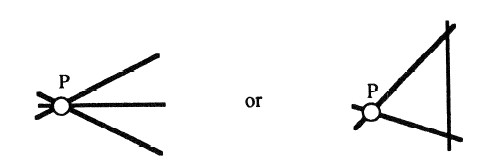
\includegraphics[width=8cm]{102.jpg}
		% \caption{初}
	\end{figure}
	(b)每一平面$\Pi \in \mathbb{P}^{3}$与S相交, 有下列3种情况:
	
	(i)不可约三次曲面;或(ii)一条圆锥曲线加上一条直线;或(iii)三条不同的直线	
	
	\textbf{证明} \ (a)若$l\in S$,则$l=T_{P}l\subset T_{P}S$, 所以$ S $中所有过$ P $的直线都包含在平面$T_{P}S$内;由(b)知最多有3个.
	
	(b)证明多重线是不可能的:如果$\Pi:(T = 0)$和$l:(Z = 0)\in \Pi$,那么称$ l $是$S\cap \Pi$的多重线意味着$ f $的形式是
	\begin{equation*}
	f=Z^{2}\cdot A(X,Y,Z,T)+T\cdot B(X,Y,Z,T)
	\end{equation*}
	其中$ A $是线性型, $ B $是二次型.那么$ S:(f=0) $在$ Z=T=B=0 $的点处是奇异的, 这是一个非空集, 因为它是$ B $在直线$ l:(Z = T = 0) $上的根集.
	
	\section{}
	\textbf{定理} \ 至少有一条直线$l$在$ S $上.
	
	有几种方法证明. 一个标准的方法是通过数维数证明:$\mathbb{P}^{3}$中的直线由4维变量参数化的,并且直线$ l $位于$ S $上要满足4个条件(因为$ f $对$ l $的限制是一个三次型,它的4个系数必须为零)
	需要做一点工作把这变成一个严格的证明, 因为它先验地只显示了这组直线的维数$\geq 0$, 并不是说它不是空的.
	
	假设命题(只关注包含直线的三次曲面)也是完全合乎逻辑的. 通过坐标几何和消元法可以直接证明(7.2). 如果你愿意省略它,请转到(7.3).证明分为三个步骤.
	
	\textbf{步骤1} \ (初步构造)对任一点$P\in S$,$ S $和切平面$T_{P}S$的交集是一条平面三次曲线$C=S\cap T_{P}S$,显然它在点$ P $处是奇异的.假设$ C $是不可约的,否则$ P $在$ S $的直线上;那么$ C $是结点或尖点三次曲线,可以选择合适的坐标$ (X,Y,Z,T) $使
	$T_{P}S:(T=0),P=(0,0,1,0)$且
	\begin{equation*}
	C:(XYZ=X^{3}+Y^{3}) \ \text{或} (X^{2}=Y{3})
	\end{equation*}
	
	对于给定的$ P, C $是结点还是尖点取决于$ f $在$ P $处的二阶导数矩阵(或海森矩阵).为简化,下面在尖点的情况下证明(7.2);
	原则上,证明在结点的情况也行得通,但消去计算会更难一些.因此假设
	\begin{equation*}
	f=X^{2}Z-Y^{3}+gT
	\end{equation*}
	其中$g=g_{2}(X,Y,Z,T)$是二次型;由$ S $在$ P $处的非奇异性知$g(0,0,1,0)\neq 0$,可以假设$g(0,0,1,0)= 0$.
	
	\textbf{步骤2} \ (主要断言的叙述)考虑$C\subset S$上的动点$P_{\alpha}=(1,\alpha,\alpha^{3},0)$.  $\mathbb{P} ^{3}$中任意过$P_{\alpha}$的直线与补平面$\Pi:(X=0)$相交于一点$ Q=(0,Y,Z,T) $.我把直线$P_{\alpha}Q$包含在$ S $中的方程写成$\alpha$和$ Q $的形式;展开
	$f(\lambda P_{\alpha}+\mu Q)$的$\lambda $和 $\mu$ 次幂得到
	\begin{equation*}
	P_{\alpha}\subset S \Leftrightarrow A(Y,Z,T)=B(Y,Z,T)=C(Y,Z,T)=0
	\end{equation*}
	其中$ A,B,C $分别是$ (X,Y,T) $的1,2,3次型,它们的系数包含$\alpha$.
	
	\textbf{主要断言} \ 存在一个"结果的"多项式$R_{27}(\alpha)$, 是$\alpha$的27次幂的首一的函数,比如
	\begin{equation*}
	R(\alpha)=0 \Leftrightarrow A=B=C=0 \text{在} \mathbb{P} ^{2} \text{中有一个共同的零点}(\eta:\zeta:\tau)
	\end{equation*}
	
	这个叙述证明了(7.2),因为它意味着对$ R $的每一个根$\alpha$,存在$\Pi$中的一点$Q=(0:\eta:\zeta:\tau)$使直线$P_{\alpha}Q$包含在S中.这个想法是一个在
	\textit{练习1.10}上的标准的消除计算;剩余的证明过程要精确地写出$ A,B,C $, 去证明断言.
	
	\textbf{步骤3} \ (极坐标形式)定义$ f $的极坐标为由
	\begin{equation*}
	f_{1}(X,Y,Z,T;X^{'},Y^{'},Z^{'},T^{'})=\dfrac{\partial f}{\partial X}\cdot X^{'}+\dfrac{\partial f}{\partial Y}\cdot Y^{'}+\dfrac{\partial f}{\partial Z}\cdot Z^{'}+\dfrac{\partial f}{\partial T}\cdot T^{'}
	\end{equation*}
	给出的两组变量$ (X,Y,Z,T) $和$(X^{'},Y^{'},Z^{'},T^{'})$的形式.
	
	从切空间的定义(见(6.4)和(6.10))可以看到对$ P=(X,Y,Z,T)\in S $和$P\neq Q=(X^{'},Y^{'},Z^{'},T^{'})\in \mathbb{P} ^{3}$,
	\begin{equation*}
	f_{1}(P;Q)=0\Leftrightarrow \text{直线$ PQ $是$ S $在点$ P $处的切线}	
	\end{equation*}
	
	显然
	\begin{equation*}
	f(\lambda P_{\alpha}+\mu Q)=\lambda^{3}f(P)+\lambda^{2}\mu f_{1}(P;Q)+\lambda \mu^{2}f_{1}(Q;P)+\mu^{3}f(Q)
	\end{equation*}
	
	所以,对$P\neq Q \in \mathbb{P} ^{3}$,4个条件$f(P)=f_{1}(P;Q)=f_{1}(Q;P)=f(Q)$是包含在$ S:(f=0) $的直线$l=PQ$的方程.几何上,称$l$是$ S $在$ P $和$ Q $点的切线,所以$f|_{l}$在这两个点处都有
	重根,根据定理1.8则有$l\subset S$.
	
	$f=X^{2}Z-Y^{3}+gT$的极坐标是
	\begin{equation*}
	f_{1}=2XZ\cdot X^{'}-3Y^{2}\cdot Y^{'}+X^{2}\cdot Z^{'}+g(X,Y,Z,T)\cdot T^{'}+Tg_{1}
	\end{equation*}
	
	这里$g_{1}=g_{1}(X,Y,Z,T;X^{'},Y^{'},Z^{'},T^{'})$是和上面定义方式相同的$ g $的极坐标形式;因为$ g $是二次的,所以$g_{1}$是一个对称的双线性型,
	使得$g_{1}(P,P)=2g(P)$.
	
	把$P_{\alpha}=(1,\alpha,\alpha^{3},0)$和$Q=(0,Y,Z,T)$代入,得到$P_{\alpha}Q \subset S $的方程为$ A=B=C=0 $,其中
	
	\begin{equation*}
	A=Z-3\alpha^{2}Y+g(1,\alpha,\alpha^{3},0)T
	\end{equation*}
	\begin{equation*}
	B=-3\alpha Y^{2}+g_{1}(1,\alpha,\alpha^{3},0;0,Y,Z,T)T
	\end{equation*}
	\begin{equation*}
	C=-Y^{3}+g(0,Y,Z,T)T
	\end{equation*}
	
	\textbf{步骤4} \ (消除计算)我现在从以上三个方程中消除$ Y,Z,T $,关注$\alpha$的最高次项.因为$ g(0,0,1,0)=1 $,所以
	\begin{equation*}
	g(1,\alpha,\alpha^{3},0)=\alpha^{6}+\cdots =a^{(6)}
	\end{equation*}
	其中$\cdots$表示$\alpha$次数低于6的项,因此$a^{(6)}$是次数为6的首一多项式.则$ A=0 $得出$ Z $是$ Y $和$ T $的线性型
	\begin{equation*}
	Z=3\alpha^{2}Y-a^{(6)}T
	\end{equation*}
	将$ B $带入,有$g_{1}$的双线性性得出
	\begin{equation*}
	B=-3\alpha Y^{2}+g_{1}(1,\alpha,\alpha^{3},0;0,Y,3\alpha^{2}Y-a^{(6)}T,T)T=b_{0}Y^{2}+b_{1}YT+b_{2}T^{2}
	\end{equation*}
	其中
	\begin{equation*}
	b_{0}=-3\alpha, b_{1}=g_{1}(1,\alpha,\alpha^{3},0;0,1,3\alpha^{2},0)=6\alpha^{5}+\cdots,
	\end{equation*}
	\begin{equation*}
	b_{2}=g_{1}(1,\alpha,\alpha^{3},0;0,0,-a^{(6)},1)=-2\alpha^{9}+\cdots
	\end{equation*}
	
	类似地,把$ Z $带入$ C $中,展开二次形式$ g $得到
	\begin{equation*}
	C=-Y^{3}+g(0,Y,3\alpha^{2}Y-a^{(6)}T,T)T=c_{0}Y^{3}+c_{1}Y^{2}T+c_{2}YT^{2}+c_{3}T^{3}
	\end{equation*}
	其中
	\begin{equation*}
	c_{0}=-1, c_{1}=g(0,1,3\alpha^{2},0)=9\alpha^{4}+\cdots,
	\end{equation*}
	\begin{equation*}
	c_{2}=g_{1}(0,1,3\alpha^{2},0;0,0,-a^{(6)},1)=-6\alpha^{8}+\cdots
	\end{equation*}
	\begin{equation*}
	c_{3}=g(0,0,-a^{(6)},1)=\alpha^{12}+\cdots
	\end{equation*}
	
	由\textit{练习1.10}的结果知,$B{'}$和$C{'}$有公共零点$(\eta:\tau)$当且仅当
	
	\[
	det\left|\begin{array}{cccccc}
	b_{0} &  b_{1} & b_{2}&  & \\
	  & b_{0} &  b_{1} & b_{2}&  \\
	  &   &b_{0} &  b_{1} & b_{2}\\
	c_{0} &  c_{1} & c_{2}& c_{3} & \\
	  &  c_{0} &  c_{1} & c_{2}& c_{3}
	\end{array}\right|=0
	\]
	
	这个行列式是$\alpha$的多项式,它的首项来自于取行列式每一行的首项:
	
	\[
	det\left|\begin{array}{cccccc}
	-3\alpha &  6\alpha^{5} & -2\alpha^{9}&  & \\
	  &-3\alpha &  6\alpha^{5} & -2\alpha^{9}&  \\
	  &   &-3\alpha &  6\alpha^{5} & -2\alpha^{9}\\
	-1& 9\alpha^{4} &  -6\alpha^{8} & \alpha^{12}& \\
	  &  -1& 9\alpha^{4} &  -6\alpha^{8} & \alpha^{12}
	\end{array}\right|=\alpha^{27}\cdot det
	\left|\begin{array}{cccccc}
	-3&  6 & -2&  & \\
	  &-3 &  6 & -2&  \\
	  &   &-3&  6 & -2\\
	-1& 9 &  -6& 1& \\
	  &  -1& 9 &  -6& 1
	\end{array}\right|=\alpha^{27}
	\]
	
	这里结束了主要断言的证明.
	\section{命题}
	
	给定一条直线$l\subset S$, 恰好存在$ S $中的5对直线$(l_{i},l^{'}_{i})$与$l$相交,且
	
	(i)对$i=1,\cdots ,5, l\cup l_{i} \cup l^{'}_{i}$是共面的
	
	(ii)$i\neq j, (l_{i} \cup l^{'}_{i})\cap(l_{j} \cup l^{'}_{j})= \varnothing $
	
	\textbf{证明} \ 如果$\Pi$是$\mathbb{P}^{3}$中的一个包含$l$的平面,那么$\Pi\cap S=l+\text{二次曲面}$(因为$f|_{\Pi}$可被$l$的方程整除).这个二次曲面可能是奇异的,也可能是非奇异的:
	\begin{figure}[H]
		\centering
		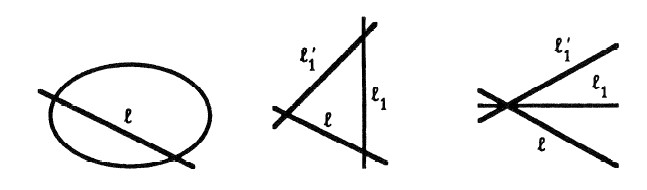
\includegraphics[width=8cm]{106.jpg}
		% \caption{初}
	\end{figure}
	我必须证明恰好有5个不同的平面$\Pi_{i} \supset l $在其中发生了奇异情况.作为性质(ii)陈述的不同平面上的直线是不相交的,可从(7.1,a)推出.
	
	假设$l:(Z=T=0)$;那么可以将$ f $展开为
	\begin{equation*}
	f=AX^{2}+BXY+CY^{2}+DX+EY+F \tag{$*$}
	\end{equation*}
	其中$A,B,C,D,E,F\in k[Z,T]$,$ A,B,C $是线性型,$ D,E $是二次型,$ f $是三次型.
	
	我把这个方程看做$ X $和$ Y $的变量二次曲线,它是奇异的当且仅当
	\begin{equation*}
	det\left|\begin{array}{ccc}
	A &  \dfrac{1}{2}B & \dfrac{1}{2} D\\
	\dfrac{1}{2}B & C &  \dfrac{1}{2} E \\
	\dfrac{1}{2} D & \dfrac{1}{2} E &  F\\
	
	\end{array}\right|=0
	\end{equation*}
	当且仅当
	\begin{equation*}
	\bigtriangleup(Z,T)
	=4ACF+BDE-AE^{2}-B^{2}F-CD^{2}=0
	\end{equation*}
	
	(特征不为2时,$\bigtriangleup$是通常行列式的4倍;特征不为2时,也容易证明)
	
	更确切地说,任何通过$l$的平面都是由$\Pi:(\mu Z=\lambda T)$给出的;如果$\mu \neq 0$,可以假设$\mu=1$,所以$Z=\lambda T$,那么根据$\Pi$上的齐次坐标$f|_{\Pi}=T \cdot Q(X,Y,T)$,其中
	\begin{equation*}
	Q=A(\lambda,1)X^{2}+B(\lambda,1)XY+C(\lambda,1)Y^{2}+D(\lambda,1)TX+E(\lambda,1)TY+F(\lambda,1)T^{2}
	\end{equation*}
	
	$\bigtriangleup(Z,T)$是五次齐次的,由(1.8),方程包括重根在内有5个根,为证明这个定理,我需要证明它没有重根,这也是$ S $的非奇异性的一个结果.
	
	\textbf{断言} \ $\bigtriangleup(Z,T)$只有单根.
	
	假设(Z=0)是$\bigtriangleup$的一个根,另$\Pi:(Z=0)$是对应的平面,我要证明$\bigtriangleup$不能被$Z^{2}$整除.由上图可知,$\Pi \cap S$ 是3条直线的集合,我可以根据它们是否并发来排列坐标,
	\begin{equation*}
	\text{或者}(i)l:(T=0),l_{1}:(X=0),l^{'}_{1}:(Y=0)
	\end{equation*}
	\begin{equation*}
	\text{或者}(i)l:(T=0),l_{1}:(X=0),l^{'}_{1}:(X=T)
	\end{equation*}
	
	因此,情况(i)$ ,f=XYT+Zg $,其中$ g $是二次形式,根据(*)式,这意味着$ B=T+aZ, $且$Z\mid A,C,D,E,F$.所以
	\begin{equation*}
	\bigtriangleup \equiv -T^{2}F \ mod Z^{2}
	\end{equation*}
	此外,点$P = (0,0,0,1)\in S$, $ P $处的非奇异性意味着F必须包含系数非零的项$ZT^{2}$. 特别地,$Z^{2}$不能整除$ F $, 因此$ (Z = 0) $是$\bigtriangleup$的单根.
	情况(ii)是类似的计算.
	
	\section{推论}
	(a)存在两条不相交的直线$l,m \subset S$.
	
	(b)$ S $是有理的(即和$\mathbb{P}^{2}$是双有理的).
	
	\textbf{证明} \ (a)根据(7.3 \ ii),取$l_{1}$和$l_{2}$.
	
	(b)考虑两条不相交的直线$l,m\subset S$,定义有理映射
	
	\begin{equation*}
	\varphi :S\rightarrow l \times m  \  \text{和} \ \psi :l \times m \rightarrow S
	\end{equation*}
	
	如果$P\in \mathbb{P} ^{3}\setminus (l\cup m) $,那么存在唯一一条过点$ P $的直线$n$与$l$和$m$都相交:
	\begin{equation*}
	P\in n, l\cap n \neq \varnothing, m\cap n\neq  \varnothing
	\end{equation*}
	集合$\Phi(P)=(l\cap n,m\cap n)\in l\times m$,这定义了一个态射
	\begin{equation*}
	\Phi:\mathbb{P} ^{3}\setminus (l\cup m)\rightarrow l \times m
	\end{equation*}
	它的纤维在$(Q,R)\in l\times m$以上就是$\mathbb{P} ^{3}$中的直线$ QR. $定义$\varphi :S\rightarrow l \times m  $为$\Phi$限制在$ S $上.
	
	反过来,对$(Q,R)\in l \times m$,令$n$是$\mathbb{P} ^{3}$中的直线$ n=QR $. 有(7.3),S中只有有限多条直线与$l$相交,因此,对于几乎所有$ (Q,R) $的值,n与S相交于3个点$ \{P, Q, R\} $,其中$ Q $和$ R $是$l$和$m$上的给定点.因此定义$\psi:l \times m \rightarrow S $;那么$\psi$是一个有理映射,因为$ P $的坐标比是$ Q ,R $的有理函数.
	
	显然$\varphi$和$\psi$是互逆的.
	
	\section{}
	我要根据定理(7.3)给出的一条直线和5对不相交直线$(l_{i},l^{'}_{i})$找出$ S $的所有直线. 任何其他直线$n\subset S$必须恰好与$l_{i},l^{'}_{i}$ 中的一条相交$ (i = 1,...,5): $这是因为在$\mathbb{P}^{3}$中,$ n $与平面$\Pi_{i}$相交,且$\Pi_{i}\cap S=l\cup l_{i} \cup l^{'}_{i}$; $ n $不能与$l_{i}$和$l^{'}_{i}$都相交,因为这与(7.1,(a))相矛盾. 整理其余直线的关键是下面的引理, 它告诉我们$ n $由与它相交的$l_{i}$和$l^{'}_{i}$唯一决定的. 称一条直线n是一条直线$l$的截线, 如果$l\cap n \neq \varnothing$.
	
	\textbf{引理} \ 如果$l_{1},...l_{4}\subset \mathbb{P}^{3}$是不相交直线, 那么
	
	或者 4条直线$l_{i}$都在一条光滑的二次曲线上,$l_{1},...l_{4}\subset Q \subset \mathbb{P}^{3}$; 它们有无数条公共截线;
	
	或者 这4条直线$l_{i}$不位于任何一条光滑的二次曲线上,$l_{1},...l_{4}\nsubseteq Q $; 它们有1条或2条公共截线.
	
	\textbf{证明} \ 存在一个光滑的二次曲面$Q\supset l_{1},...l_{3}$: 有几种证明是可能的.
	
	然后选择恰当的坐标,$ Q:(XT - YZ),Q $有两族直线或生成元:$l_{1},...l_{3}$的任意截线一定在$ Q $中,因为它有3个点在$ Q $中.现在如果$l_{4}\nsubseteq Q$,那么$l_{4}\cap Q$={1或2个点}, 通过这些点的其它族的生成元是 $l_{1},...l_{4}$ 的所有公共截线.
	
	\begin{figure}[H]
		\centering
		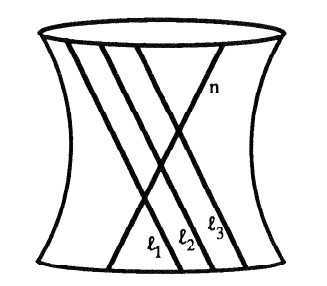
\includegraphics[width=5cm]{109.jpg}\\
		%\caption{一个简单的图例,其中'$ \leftrightarrow $'代表同构}
	\end{figure}
	\section{27条直线}
	$l$和$ m $是$ S $中两条不相交的直线,$  m $恰好与和直线 $l$相交的5对直线$(l_{i},l^{'}_{i})$的每一对中的一条相交.通过重新编号这些对直线, 假设$ m $与直线$l_{i}$相交,$ i = 1,...5 $. 对以下记号:
	
	\begin{figure}[H]
		\centering
		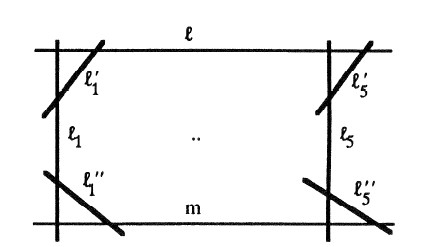
\includegraphics[width=5cm]{1092.jpg}\\
		%\caption{一个简单的图例,其中'$ \leftrightarrow $'代表同构}
	\end{figure}
	
	因此, 与$ m $相交的5对直线记为$(l_{i},l^{''}_{i})$,$ i = 1,…,5. $ 将(7.3,(ii))应用于$ m $,$i \neq j$,直线$l^{''}_{i}$与$l_{j}$不相交. 另一方面,$ S $的每一条直线一定与$l, l_{j},l^{'}_{j}$ 中的一条相交,因此$l^{''}_{i}$与$l^{'}_{j}$相交,$i\neq j$.
	
	\textbf{断言}
	(I)如果$n\subset S$是这17条直线之外的任意一条,那么$ n $恰好与5条直线$l_{1},...l_{5}$中的三条相交.
	
	(II)反之, 任意选取三个元素${i.j.k}\subset\{1,2,3,4,5\}$,有唯一的一条直线$l_{ijk}$与$l_{i},l_{j},l_{k}$相交.
	
	
	\textbf{证明} \ (I)给定$ S $中的4条不相交的直线,显然它们不都位于同一条二次曲线$ Q $上, 否则$Q\subset S$,与$ S $不可约矛盾.
	
	如果n与$l_{i}$中$\geq 4$条直线相交,那么根据引理7.5,$n=l$或$ m $,矛盾.如果n与$l_{i}$中$\leq 2$条直线相交,那么它与$l^{'}_{i}$中$\geq 3$条直线相交,所以它和$l^{'}_{2},l^{'}_{3},l^{'}_{4},l^{'}_{5}$相交,或与$l_{1},l^{'}_{3},l^{'}_{4},l^{'}_{5}$相交;
	但是根据以上论述,$l$和$l^{''}_{1}$是5条不相交直线 $l^{'}_{2},l^{'}_{3},l^{'}_{4},l^{'}_{5}$和$l_{1}$的两条共同截线,再次根据引理7.5,如果$ n $与其中的$\geq 4$条直线相交,那么$n=l$或$l^{''}_{1}$.这同样矛盾.
	
	(II)根据(7.3),有10条直线与$l_{1}$相交,现在只有4条被计数$(l,l^{'}_{1},m,l^{''}_{1})$.剩余的6条直线一定恰好与剩下4条直线$l_{2} ,l_{3} , l_{4} , l_{5}$中的2条相交.并且恰好有$6=C^{2}_{4}$种选择,所以6种情况都有.
	
	这给出了$l$的直线
	\begin{equation*}
	\{l,m,l_{i},l^{'}_{i},l^{''}_{i},l_{ijk}\}
	\end{equation*}
	它们的数量是
	\begin{equation*}
	1+1+5+5+5+10=27
	\end{equation*}
	\section{直线的结构}
	另一种说法是$ S $上的直线是$l,l_{1},l_{2},l_{3},l_{4},l_{5},l^{'}_{1},l^{'}_{2},l^{'}_{3},l^{'}_{4},l^{'}_{5}$,还有16条与
	$l_{1},l_{2},l_{3},l_{4},l_{5}$中的奇数条直线相交的直线:
	\begin{equation*}
	l^{''}_{i} \text{只与} l_{i}\text{相交}
	\end{equation*}
	\begin{equation*}
	l_{ijk} \text{只与}l_{i},l_{j},l_{k}\text{相交}
	\end{equation*}
	\begin{equation*}
	m\text{与}l_{1},...l_{5}\text{中所有直线相交}
	\end{equation*}
	在介绍过的符号中,很容易看出$ S $的27条直线之间的关系如下:
	
	$l\text{与}l_{1},l_{2},l_{3},l_{4},l_{5},l^{'}_{1},l^{'}_{2},l^{'}_{3},l^{'}_{4},l^{'}_{5}\text{相交}$;
	
	$l_{1}\text{与}l,m,l^{'}_{1},l^{''}_{1}\text{和}l_{1jk}(6\text{种选择}\{j,k\}\subset \{2,3,4,5\})\text{相交}$;
	
	$l^{'}_{1}\text{与}l,l_{1},l^{''}_{j}(4种选择j\neq 1)\text{和}l_{ijk}(4\text{种选择}\{i,j,k\}\subset \{2,3,4,5\})\text{相交}$;
	
	$l^{''}_{1}\text{与}m,l_{1},l^{'}_{j}(4种选择j\neq 1)\text{和}l_{ijk}(4\text{种选择}\{i,j,k\}\subset \{2,3,4,5\})\text{相交}$;
	
	$l_{123}\text{与}l_{1},l_{2},l_{3},l_{145},l_{245},l_{345}, l^{'}_{4},l^{'}_{5},l^{''}_{4},l^{''}_{5}\text{相交}$;
	这个组合构型有许多不同的表示,其中一些比这里给出的对称得多.
	
\end{document}
